% Chapter 0: Refresher and inference for dependent data
% Advanced Time Series Analysis and Forecasting -- Master's programme Applied Statistics and Data Science, year 1, semester 2, Bucharest University of Economic Studies
% GENERATED by latex/build_chapter0.py -- edit the generator, not this file.

\newcommand{\coursename}{Advanced Time Series Analysis and Forecasting}
% Preambul comun ATS -- Analiza avansată a seriilor de timp și previziune / Advanced Time Series Analysis and Forecasting
% (Beamer, 16:9). Același design ca MFM, SFM și TSA (copiat din TSA, 5 octombrie 2026). Înainte de % Preambul comun ATS -- Analiza avansată a seriilor de timp și previziune / Advanced Time Series Analysis and Forecasting
% (Beamer, 16:9). Același design ca MFM, SFM și TSA (copiat din TSA, 5 octombrie 2026). Înainte de % Preambul comun ATS -- Analiza avansată a seriilor de timp și previziune / Advanced Time Series Analysis and Forecasting
% (Beamer, 16:9). Același design ca MFM, SFM și TSA (copiat din TSA, 5 octombrie 2026). Înainte de \input{../../latex/preamble} se definește
%   \newcommand{\coursename}{Advanced Time Series Analysis and Forecasting}          (EN)
%   \newcommand{\coursename}{Analiza avansată a seriilor de timp și previziune}       (RO)  și  \def\atslang{ro}
% Fișierele .tex se află în EN/Courses, EN/Seminars, RO/Cursuri, RO/Seminarii (două niveluri sub rădăcină).
% Deck-urile sînt generate de latex/build_chapterN.py / build_seminarN.py (vezi latex/ats_build.py).

\documentclass[9pt, aspectratio=169, t]{beamer}
\providecommand{\coursename}{Advanced Time Series Analysis and Forecasting}

% Ensure content fits on slides
\setbeamersize{text margin left=8mm, text margin right=8mm}
% Smaller institute font (title page)
\setbeamerfont{institute}{size=\footnotesize}

%=============================================================================
% THEME AND STYLE CONFIGURATION
%=============================================================================
\usetheme{default}
% Using default theme for clean header/footer control

% Color Palette (matching Redispatch PDF)
\definecolor{MainBlue}{RGB}{26, 58, 110}
\definecolor{AccentBlue}{RGB}{26, 58, 110}
\definecolor{IDAred}{RGB}{205, 0, 0}
\definecolor{DarkGray}{RGB}{51, 51, 51}
\definecolor{MediumGray}{RGB}{128, 128, 128}
\definecolor{LightGray}{RGB}{248, 248, 248}
\definecolor{VeryLightGray}{RGB}{235, 235, 235}
\definecolor{KeynoteGray}{RGB}{218, 218, 218}
\definecolor{SectionGray}{RGB}{120, 120, 120}
\definecolor{FooterGray}{RGB}{100, 100, 100}
\definecolor{Crimson}{RGB}{220, 53, 69}
\definecolor{Forest}{RGB}{46, 125, 50}
\definecolor{Amber}{RGB}{181, 133, 63}
\definecolor{Orange}{RGB}{230, 126, 34}
\definecolor{Purple}{RGB}{142, 68, 173}

% Gradient background (exact Keynote 315° gradient: white to RGB 218,218,218)
\setbeamertemplate{background}{%
    \begin{tikzpicture}[remember picture, overlay]
        \shade[shading=axis, shading angle=315,
        top color=white, bottom color=KeynoteGray]
        (current page.south west) rectangle (current page.north east);
    \end{tikzpicture}%
}
% Fallback solid color for compatibility
\setbeamercolor{background canvas}{bg=}

\setbeamercolor{palette primary}{bg=MainBlue, fg=white}
\setbeamercolor{palette secondary}{bg=MainBlue!85, fg=white}
\setbeamercolor{palette tertiary}{bg=MainBlue!70, fg=white}
\setbeamercolor{structure}{fg=MainBlue}
\setbeamercolor{title}{fg=IDAred}
\setbeamercolor{frametitle}{fg=IDAred, bg=}
\setbeamercolor{block title}{bg=MainBlue, fg=white}
\setbeamercolor{block body}{bg=VeryLightGray, fg=DarkGray}
\setbeamercolor{block title alerted}{bg=Crimson, fg=white}
\setbeamercolor{block body alerted}{bg=Crimson!8, fg=DarkGray}
\setbeamercolor{block title example}{bg=Forest, fg=white}
\setbeamercolor{block body example}{bg=Forest!8, fg=DarkGray}
\setbeamercolor{item}{fg=MainBlue}

% Footer colors (override Madrid theme blue)
\setbeamercolor{author in head/foot}{fg=FooterGray, bg=}
\setbeamercolor{title in head/foot}{fg=FooterGray, bg=}
\setbeamercolor{date in head/foot}{fg=FooterGray, bg=}
\setbeamercolor{section in head/foot}{fg=FooterGray, bg=}
\setbeamercolor{subsection in head/foot}{fg=FooterGray, bg=}

% Bullet styles (apply everywhere including blocks)
\setbeamertemplate{itemize item}{\color{MainBlue}$\boxdot$}
\setbeamertemplate{itemize subitem}{\color{MainBlue}$\blacktriangleright$}
\setbeamertemplate{itemize subsubitem}{\color{MainBlue}\tiny$\bullet$}
\setbeamertemplate{itemize/enumerate body begin}{\normalsize}
\setbeamertemplate{itemize/enumerate subbody begin}{\normalsize}

% Item spacing - compact style
\setlength{\leftmargini}{10pt}       % Level 1: minimal indent
\setlength{\leftmarginii}{10pt}      % Level 2: minimal additional indent
% Compact list spacing (zero extra space before/after lists in blocks)
\makeatletter
\def\@listi{\leftmargin\leftmargini \topsep 0pt \parsep 0pt \itemsep 0pt}
\def\@listii{\leftmargin\leftmarginii \topsep 0pt \parsep 0pt \itemsep 0pt}
\makeatother

\setbeamertemplate{navigation symbols}{}

%=============================================================================
% CUSTOM HEADLINE
%=============================================================================
\setbeamertemplate{headline}{%
    \vskip10pt%
    \hbox to \paperwidth{%
        \hskip0.5cm%
        {\small\color{FooterGray}\renewcommand{\hyperlink}[2]{##2}\insertsectionhead}%
        \hfill%
        \textcolor{FooterGray}{\small\insertframenumber}%
        \hskip0.5cm%
    }%
    \vskip4pt%
    {\color{FooterGray}\hrule height 0.4pt}%
}

%=============================================================================
% CUSTOM FOOTER
%=============================================================================
\usepackage{fontawesome5}

\setbeamertemplate{footline}{%
    {\color{FooterGray}\hrule height 0.4pt}%
    \vskip4pt%
    \hbox to \paperwidth{%
        \hskip0.5cm%
        \textcolor{FooterGray}{\small\coursename}%
        \hfill%
        \raisebox{-0.1em}{%
            \begin{tikzpicture}[x=0.08em, y=0.08em, line width=0.4pt]
                \draw[FooterGray] (0,3) -- (1,4) -- (2,3.5) -- (3,5) -- (4,4) -- (5,6) -- (6,5.5) -- (7,4) -- (8,5) -- (9,7) -- (10,6) -- (11,5) -- (12,6.5) -- (13,8) -- (14,7) -- (15,6) -- (16,7.5) -- (17,9) -- (18,8) -- (19,7) -- (20,8.5) -- (21,10) -- (22,9) -- (23,8) -- (24,9.5);
            \end{tikzpicture}%
        }%
        \hskip0.5cm%
    }%
    \vskip6pt%
}

%=============================================================================
% PACKAGES
%=============================================================================
\usepackage[utf8]{inputenc}
\DeclareUnicodeCharacter{03B1}{\ensuremath{\alpha}}
\usepackage[T1]{fontenc}
\usepackage{amsmath, amssymb, amsthm}
\usepackage{mathtools}
\usepackage{bm}
\usepackage{tikz}
\usetikzlibrary{arrows.meta, positioning, shapes, calc, decorations.pathreplacing, shadings}
\usepackage{booktabs}
\usepackage{multirow}
\usepackage{array}
\usepackage{graphicx}
\usepackage{animate}
\usepackage{hyperref}
\usepackage{colortbl}
\usepackage{listings}
\lstset{language=Python, basicstyle=\ttfamily\scriptsize, keywordstyle=\color{MainBlue}\bfseries,
  commentstyle=\color{Forest}, stringstyle=\color{Crimson}, breaklines=true,
  frame=none, backgroundcolor=\color{VeryLightGray}, xleftmargin=2mm}
\hypersetup{colorlinks=true, linkcolor=MainBlue, urlcolor=MainBlue}
\graphicspath{{../../logos/}{../../charts/}{../../photos/}}
\usepackage{xcolor}
\hfuzz=2pt  % Suppress tiny overfull warnings (<2pt)
\vfuzz=2pt  % Suppress tiny vertical overfull warnings (<2pt)

%=============================================================================
% QUANTLET COMMANDS
%   \quantlet{<displayed name>}{<url>}       (generic)
%   \atsquantlet{Ch_05}{ATS_ch5_garch}       -> https://github.com/danpele/Advanced-Time-Series/tree/main/Quantlets/Ch_05/ATS_ch5_garch
%   \qlurl{<folder>} is defined per chapter by the generator (Quantlets/Ch_NN/<folder>)
%=============================================================================
\newcommand{\atsrepo}{https://github.com/danpele/Advanced-Time-Series}
\newcommand{\atsqlbase}{https://github.com/danpele/Advanced-Time-Series/tree/main/Quantlets}
\newcommand{\quantlet}[2]{%
    \hfill\href{#2}{%
        \raisebox{-0.15em}{
\includegraphics[height=0.7em]{ql_logo.png}}%
        \textcolor{MainBlue}{\tiny\ #1}%
    }%
}
\newcommand{\atsquantlet}[2]{\quantlet{\detokenize{#2}}{\atsqlbase/#1/#2}}

%=============================================================================
% NOTEBOOKS (Google Colab)
%   \colaburl{notebooks/EN/chapter5_seminar_notebook.ipynb} -> the Colab link of a file in the ATS repo
%   \nb: the chapter notebook (each seminar deck redefines it with \renewcommand)
%=============================================================================
\newcommand{\colaburl}[1]{https://colab.research.google.com/github/danpele/Advanced-Time-Series/blob/main/#1}
\newcommand{\nb}{https://colab.research.google.com/github/danpele/Advanced-Time-Series/tree/main/notebooks/EN}
\newcommand{\nbname}{notebooks/EN}

%=============================================================================
% SLIDE HELPERS (used by the generators; the same as in MFM)
%=============================================================================
% local font size for list bodies (the preamble forces \normalsize)
\newcommand{\itemsize}[1]{\setbeamertemplate{itemize/enumerate body begin}{#1}\setbeamertemplate{itemize/enumerate subbody begin}{#1}}
\newcommand{\intitle}[1]{{\hypersetup{urlcolor=white}#1}}   % white links inside coloured title bars
\newcommand{\imgcap}[1]{{\scriptsize #1}\\[0.5mm]}          % caption under a photo
\newcommand{\imgcredit}[2]{{\tiny\color{FooterGray}\href{#1}{#2}}}   % image credit: source URL, author/licence
\newcommand{\aiprompt}[1]{{\ttfamily\color{MainBlue}#1}}     % a prompt to an AI assistant

%=============================================================================
% SEMINARS: student version by default; the instructor wrapper *_solutions.tex sets \solutionstrue
%=============================================================================
\makeatletter\@ifundefined{ifsolutions}{\expandafter\newif\csname ifsolutions\endcsname}{}\makeatother
\newcommand{\solonly}[1]{\ifsolutions #1\fi}
\newcommand{\propsub}{\ifsolutions\else\framesubtitle{\ifdefined\atslang Rezolvarea se discută la seminar\else Solution discussed in class\fi}\fi}

%=============================================================================
% APPENDIX AND CHAPTER LINKS (latex/appendix_links.py writes the calls; it also re-declares these
% macros before \begin{document}, so the decks compile with or without this preamble block)
%=============================================================================
\providecommand{\atsapplink}[3]{\hypertarget{#2}{}\hyperlink{#1}{\beamergotobutton{#3}}}
\providecommand{\atsappback}[2]{\begin{tikzpicture}[remember picture,overlay]\node[anchor=south east] at ([xshift=-3mm,yshift=7mm]current page.south east){\hyperlink{#1}{\beamerreturnbutton{#2}}};\end{tikzpicture}}
\providecommand{\atschlink}[2]{\href{#1}{#2}}
\providecommand{\atschlinkt}[2]{\href{#1}{\usebeamercolor[fg]{frametitle}#2}}

%=============================================================================
% QUANTINAR COMMAND: link către un curs Quantinar (subiecte avansate)
%=============================================================================
\newcommand{\quantinar}[2]{%
    \href{#2}{%
        \raisebox{-0.15em}{
\includegraphics[height=0.8em]{qr_logo.png}}%
        \textcolor{MainBlue}{\scriptsize\ #1}%
    }%
}

%=============================================================================
% CUSTOM TITLE PAGE
%=============================================================================
\defbeamertemplate*{title page}{hybrid}[1][]
{
    \vspace{0.2cm}
    % Logos row - top header (with clickable links)
    \begin{center}
        \href{https://www.ase.ro}{
\includegraphics[height=1.0cm]{ase_logo.png}}\hspace{0.3cm}%
        \href{https://theida.net}{
\includegraphics[height=1.0cm]{ida_logo.png}}\hspace{0.3cm}%
        \href{https://blockchain-research-center.com}{
\includegraphics[height=1.0cm]{brc_logo.png}}\hspace{0.3cm}%
        \href{https://www.ai4efin.ase.ro}{
\includegraphics[height=1.0cm]{ai4efin_logo.png}}\hspace{0.3cm}%
        \href{https://ipe.ro/new}{
\includegraphics[height=1.0cm]{acad_logo.png}}\hspace{0.3cm}%
        \href{https://www.digital-finance-msca.com}{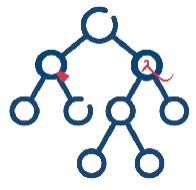
\includegraphics[height=1.0cm]{msca_logo.png}}%
    \end{center}

    \vspace{0.6cm}

    % Main title with Q logos on sides (with clickable links)
    \begin{center}
        \begin{minipage}{0.1\textwidth}
            \centering
            \href{https://quantlet.com}{
\includegraphics[height=1.1cm]{ql_logo.png}}
        \end{minipage}%
        \begin{minipage}{0.78\textwidth}
            \centering
            {\LARGE\bfseries\usebeamercolor[fg]{title}\inserttitle}

            \vspace{0.3cm}

            {\usebeamerfont{subtitle}\usebeamercolor[fg]{title}\insertsubtitle}
        \end{minipage}%
        \begin{minipage}{0.1\textwidth}
            \centering
            \href{https://quantinar.com}{
\includegraphics[height=1.1cm]{qr_logo.png}}
        \end{minipage}
    \end{center}

    \vspace{0.6cm}

    % Authors (left aligned)
    \hspace{0.5cm}{\usebeamerfont{author}\insertauthor}

    \vspace{0.3cm}

    % Institute/Affiliations (left aligned)
    \hspace{0.5cm}\begin{minipage}[t]{0.9\textwidth}
        \raggedright\small\insertinstitute
    \end{minipage}
}

%=============================================================================
% THEOREM ENVIRONMENTS
%=============================================================================
\theoremstyle{definition}
\setbeamertemplate{theorems}[numbered]
\ifdefined\atslang
\newtheorem{defn}{Definiție}
\newtheorem{thm}{Teoremă}
\newtheorem{prop}{Propoziție}
\newtheorem{rmk}{Observație}
\else
\newtheorem{defn}{Definition}
\newtheorem{thm}{Theorem}
\newtheorem{prop}{Proposition}
\newtheorem{rmk}{Remark}
\fi

%=============================================================================
% CENTRED MINIPAGE (no extra vertical space)
%=============================================================================
\newenvironment{cminipage}[1]{%
    \par\noindent\hfill\begin{minipage}{#1}\ignorespaces
}{%
    \end{minipage}\hfill\null\par
}

%=============================================================================
% CUSTOM COMMANDS
%=============================================================================
\newcommand{\E}{\mathbb{E}}
\newcommand{\Var}{\text{Var}}
\newcommand{\Cov}{\text{Cov}}
\newcommand{\Corr}{\text{Corr}}
\newcommand{\R}{\mathbb{R}}
\newcommand{\N}{\mathbb{N}}
\newcommand{\Z}{\mathbb{Z}}
\newcommand{\B}{\mathbf{B}}
\newcommand{\imark}{\textcolor{MainBlue}{\textbullet}}
\newcommand{\RMSE}{\text{RMSE}}
\newcommand{\MAE}{\text{MAE}}
\newcommand{\MAPE}{\text{MAPE}}

% Boldface vector/matrix commands (VAR, VECM, state space)
\newcommand{\bY}{\mathbf{Y}}
\newcommand{\bX}{\mathbf{X}}
\newcommand{\bA}{\mathbf{A}}
\newcommand{\bB}{\mathbf{B}}
\newcommand{\bepsilon}{\boldsymbol{\varepsilon}}
\newcommand{\bSigma}{\boldsymbol{\Sigma}}
\newcommand{\bPhi}{\boldsymbol{\Phi}}
\newcommand{\bGamma}{\boldsymbol{\Gamma}}
\newcommand{\bPi}{\boldsymbol{\Pi}}
\newcommand{\bc}{\mathbf{c}}
\newcommand{\balpha}{\boldsymbol{\alpha}}
\newcommand{\bbeta}{\boldsymbol{\beta}}
\newcommand{\bvarepsilon}{\boldsymbol{\varepsilon}}

% Seminar marks
\newcommand{\correct}{\textcolor{Forest}{\checkmark}}
\newcommand{\incorrect}{\textcolor{Crimson}{\texttimes}}
 se definește
%   \newcommand{\coursename}{Advanced Time Series Analysis and Forecasting}          (EN)
%   \newcommand{\coursename}{Analiza avansată a seriilor de timp și previziune}       (RO)  și  \def\atslang{ro}
% Fișierele .tex se află în EN/Courses, EN/Seminars, RO/Cursuri, RO/Seminarii (două niveluri sub rădăcină).
% Deck-urile sînt generate de latex/build_chapterN.py / build_seminarN.py (vezi latex/ats_build.py).

\documentclass[9pt, aspectratio=169, t]{beamer}
\providecommand{\coursename}{Advanced Time Series Analysis and Forecasting}

% Ensure content fits on slides
\setbeamersize{text margin left=8mm, text margin right=8mm}
% Smaller institute font (title page)
\setbeamerfont{institute}{size=\footnotesize}

%=============================================================================
% THEME AND STYLE CONFIGURATION
%=============================================================================
\usetheme{default}
% Using default theme for clean header/footer control

% Color Palette (matching Redispatch PDF)
\definecolor{MainBlue}{RGB}{26, 58, 110}
\definecolor{AccentBlue}{RGB}{26, 58, 110}
\definecolor{IDAred}{RGB}{205, 0, 0}
\definecolor{DarkGray}{RGB}{51, 51, 51}
\definecolor{MediumGray}{RGB}{128, 128, 128}
\definecolor{LightGray}{RGB}{248, 248, 248}
\definecolor{VeryLightGray}{RGB}{235, 235, 235}
\definecolor{KeynoteGray}{RGB}{218, 218, 218}
\definecolor{SectionGray}{RGB}{120, 120, 120}
\definecolor{FooterGray}{RGB}{100, 100, 100}
\definecolor{Crimson}{RGB}{220, 53, 69}
\definecolor{Forest}{RGB}{46, 125, 50}
\definecolor{Amber}{RGB}{181, 133, 63}
\definecolor{Orange}{RGB}{230, 126, 34}
\definecolor{Purple}{RGB}{142, 68, 173}

% Gradient background (exact Keynote 315° gradient: white to RGB 218,218,218)
\setbeamertemplate{background}{%
    \begin{tikzpicture}[remember picture, overlay]
        \shade[shading=axis, shading angle=315,
        top color=white, bottom color=KeynoteGray]
        (current page.south west) rectangle (current page.north east);
    \end{tikzpicture}%
}
% Fallback solid color for compatibility
\setbeamercolor{background canvas}{bg=}

\setbeamercolor{palette primary}{bg=MainBlue, fg=white}
\setbeamercolor{palette secondary}{bg=MainBlue!85, fg=white}
\setbeamercolor{palette tertiary}{bg=MainBlue!70, fg=white}
\setbeamercolor{structure}{fg=MainBlue}
\setbeamercolor{title}{fg=IDAred}
\setbeamercolor{frametitle}{fg=IDAred, bg=}
\setbeamercolor{block title}{bg=MainBlue, fg=white}
\setbeamercolor{block body}{bg=VeryLightGray, fg=DarkGray}
\setbeamercolor{block title alerted}{bg=Crimson, fg=white}
\setbeamercolor{block body alerted}{bg=Crimson!8, fg=DarkGray}
\setbeamercolor{block title example}{bg=Forest, fg=white}
\setbeamercolor{block body example}{bg=Forest!8, fg=DarkGray}
\setbeamercolor{item}{fg=MainBlue}

% Footer colors (override Madrid theme blue)
\setbeamercolor{author in head/foot}{fg=FooterGray, bg=}
\setbeamercolor{title in head/foot}{fg=FooterGray, bg=}
\setbeamercolor{date in head/foot}{fg=FooterGray, bg=}
\setbeamercolor{section in head/foot}{fg=FooterGray, bg=}
\setbeamercolor{subsection in head/foot}{fg=FooterGray, bg=}

% Bullet styles (apply everywhere including blocks)
\setbeamertemplate{itemize item}{\color{MainBlue}$\boxdot$}
\setbeamertemplate{itemize subitem}{\color{MainBlue}$\blacktriangleright$}
\setbeamertemplate{itemize subsubitem}{\color{MainBlue}\tiny$\bullet$}
\setbeamertemplate{itemize/enumerate body begin}{\normalsize}
\setbeamertemplate{itemize/enumerate subbody begin}{\normalsize}

% Item spacing - compact style
\setlength{\leftmargini}{10pt}       % Level 1: minimal indent
\setlength{\leftmarginii}{10pt}      % Level 2: minimal additional indent
% Compact list spacing (zero extra space before/after lists in blocks)
\makeatletter
\def\@listi{\leftmargin\leftmargini \topsep 0pt \parsep 0pt \itemsep 0pt}
\def\@listii{\leftmargin\leftmarginii \topsep 0pt \parsep 0pt \itemsep 0pt}
\makeatother

\setbeamertemplate{navigation symbols}{}

%=============================================================================
% CUSTOM HEADLINE
%=============================================================================
\setbeamertemplate{headline}{%
    \vskip10pt%
    \hbox to \paperwidth{%
        \hskip0.5cm%
        {\small\color{FooterGray}\renewcommand{\hyperlink}[2]{##2}\insertsectionhead}%
        \hfill%
        \textcolor{FooterGray}{\small\insertframenumber}%
        \hskip0.5cm%
    }%
    \vskip4pt%
    {\color{FooterGray}\hrule height 0.4pt}%
}

%=============================================================================
% CUSTOM FOOTER
%=============================================================================
\usepackage{fontawesome5}

\setbeamertemplate{footline}{%
    {\color{FooterGray}\hrule height 0.4pt}%
    \vskip4pt%
    \hbox to \paperwidth{%
        \hskip0.5cm%
        \textcolor{FooterGray}{\small\coursename}%
        \hfill%
        \raisebox{-0.1em}{%
            \begin{tikzpicture}[x=0.08em, y=0.08em, line width=0.4pt]
                \draw[FooterGray] (0,3) -- (1,4) -- (2,3.5) -- (3,5) -- (4,4) -- (5,6) -- (6,5.5) -- (7,4) -- (8,5) -- (9,7) -- (10,6) -- (11,5) -- (12,6.5) -- (13,8) -- (14,7) -- (15,6) -- (16,7.5) -- (17,9) -- (18,8) -- (19,7) -- (20,8.5) -- (21,10) -- (22,9) -- (23,8) -- (24,9.5);
            \end{tikzpicture}%
        }%
        \hskip0.5cm%
    }%
    \vskip6pt%
}

%=============================================================================
% PACKAGES
%=============================================================================
\usepackage[utf8]{inputenc}
\DeclareUnicodeCharacter{03B1}{\ensuremath{\alpha}}
\usepackage[T1]{fontenc}
\usepackage{amsmath, amssymb, amsthm}
\usepackage{mathtools}
\usepackage{bm}
\usepackage{tikz}
\usetikzlibrary{arrows.meta, positioning, shapes, calc, decorations.pathreplacing, shadings}
\usepackage{booktabs}
\usepackage{multirow}
\usepackage{array}
\usepackage{graphicx}
\usepackage{animate}
\usepackage{hyperref}
\usepackage{colortbl}
\usepackage{listings}
\lstset{language=Python, basicstyle=\ttfamily\scriptsize, keywordstyle=\color{MainBlue}\bfseries,
  commentstyle=\color{Forest}, stringstyle=\color{Crimson}, breaklines=true,
  frame=none, backgroundcolor=\color{VeryLightGray}, xleftmargin=2mm}
\hypersetup{colorlinks=true, linkcolor=MainBlue, urlcolor=MainBlue}
\graphicspath{{../../logos/}{../../charts/}{../../photos/}}
\usepackage{xcolor}
\hfuzz=2pt  % Suppress tiny overfull warnings (<2pt)
\vfuzz=2pt  % Suppress tiny vertical overfull warnings (<2pt)

%=============================================================================
% QUANTLET COMMANDS
%   \quantlet{<displayed name>}{<url>}       (generic)
%   \atsquantlet{Ch_05}{ATS_ch5_garch}       -> https://github.com/danpele/Advanced-Time-Series/tree/main/Quantlets/Ch_05/ATS_ch5_garch
%   \qlurl{<folder>} is defined per chapter by the generator (Quantlets/Ch_NN/<folder>)
%=============================================================================
\newcommand{\atsrepo}{https://github.com/danpele/Advanced-Time-Series}
\newcommand{\atsqlbase}{https://github.com/danpele/Advanced-Time-Series/tree/main/Quantlets}
\newcommand{\quantlet}[2]{%
    \hfill\href{#2}{%
        \raisebox{-0.15em}{
\includegraphics[height=0.7em]{ql_logo.png}}%
        \textcolor{MainBlue}{\tiny\ #1}%
    }%
}
\newcommand{\atsquantlet}[2]{\quantlet{\detokenize{#2}}{\atsqlbase/#1/#2}}

%=============================================================================
% NOTEBOOKS (Google Colab)
%   \colaburl{notebooks/EN/chapter5_seminar_notebook.ipynb} -> the Colab link of a file in the ATS repo
%   \nb: the chapter notebook (each seminar deck redefines it with \renewcommand)
%=============================================================================
\newcommand{\colaburl}[1]{https://colab.research.google.com/github/danpele/Advanced-Time-Series/blob/main/#1}
\newcommand{\nb}{https://colab.research.google.com/github/danpele/Advanced-Time-Series/tree/main/notebooks/EN}
\newcommand{\nbname}{notebooks/EN}

%=============================================================================
% SLIDE HELPERS (used by the generators; the same as in MFM)
%=============================================================================
% local font size for list bodies (the preamble forces \normalsize)
\newcommand{\itemsize}[1]{\setbeamertemplate{itemize/enumerate body begin}{#1}\setbeamertemplate{itemize/enumerate subbody begin}{#1}}
\newcommand{\intitle}[1]{{\hypersetup{urlcolor=white}#1}}   % white links inside coloured title bars
\newcommand{\imgcap}[1]{{\scriptsize #1}\\[0.5mm]}          % caption under a photo
\newcommand{\imgcredit}[2]{{\tiny\color{FooterGray}\href{#1}{#2}}}   % image credit: source URL, author/licence
\newcommand{\aiprompt}[1]{{\ttfamily\color{MainBlue}#1}}     % a prompt to an AI assistant

%=============================================================================
% SEMINARS: student version by default; the instructor wrapper *_solutions.tex sets \solutionstrue
%=============================================================================
\makeatletter\@ifundefined{ifsolutions}{\expandafter\newif\csname ifsolutions\endcsname}{}\makeatother
\newcommand{\solonly}[1]{\ifsolutions #1\fi}
\newcommand{\propsub}{\ifsolutions\else\framesubtitle{\ifdefined\atslang Rezolvarea se discută la seminar\else Solution discussed in class\fi}\fi}

%=============================================================================
% APPENDIX AND CHAPTER LINKS (latex/appendix_links.py writes the calls; it also re-declares these
% macros before \begin{document}, so the decks compile with or without this preamble block)
%=============================================================================
\providecommand{\atsapplink}[3]{\hypertarget{#2}{}\hyperlink{#1}{\beamergotobutton{#3}}}
\providecommand{\atsappback}[2]{\begin{tikzpicture}[remember picture,overlay]\node[anchor=south east] at ([xshift=-3mm,yshift=7mm]current page.south east){\hyperlink{#1}{\beamerreturnbutton{#2}}};\end{tikzpicture}}
\providecommand{\atschlink}[2]{\href{#1}{#2}}
\providecommand{\atschlinkt}[2]{\href{#1}{\usebeamercolor[fg]{frametitle}#2}}

%=============================================================================
% QUANTINAR COMMAND: link către un curs Quantinar (subiecte avansate)
%=============================================================================
\newcommand{\quantinar}[2]{%
    \href{#2}{%
        \raisebox{-0.15em}{
\includegraphics[height=0.8em]{qr_logo.png}}%
        \textcolor{MainBlue}{\scriptsize\ #1}%
    }%
}

%=============================================================================
% CUSTOM TITLE PAGE
%=============================================================================
\defbeamertemplate*{title page}{hybrid}[1][]
{
    \vspace{0.2cm}
    % Logos row - top header (with clickable links)
    \begin{center}
        \href{https://www.ase.ro}{
\includegraphics[height=1.0cm]{ase_logo.png}}\hspace{0.3cm}%
        \href{https://theida.net}{
\includegraphics[height=1.0cm]{ida_logo.png}}\hspace{0.3cm}%
        \href{https://blockchain-research-center.com}{
\includegraphics[height=1.0cm]{brc_logo.png}}\hspace{0.3cm}%
        \href{https://www.ai4efin.ase.ro}{
\includegraphics[height=1.0cm]{ai4efin_logo.png}}\hspace{0.3cm}%
        \href{https://ipe.ro/new}{
\includegraphics[height=1.0cm]{acad_logo.png}}\hspace{0.3cm}%
        \href{https://www.digital-finance-msca.com}{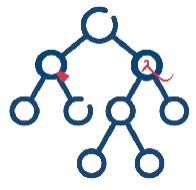
\includegraphics[height=1.0cm]{msca_logo.png}}%
    \end{center}

    \vspace{0.6cm}

    % Main title with Q logos on sides (with clickable links)
    \begin{center}
        \begin{minipage}{0.1\textwidth}
            \centering
            \href{https://quantlet.com}{
\includegraphics[height=1.1cm]{ql_logo.png}}
        \end{minipage}%
        \begin{minipage}{0.78\textwidth}
            \centering
            {\LARGE\bfseries\usebeamercolor[fg]{title}\inserttitle}

            \vspace{0.3cm}

            {\usebeamerfont{subtitle}\usebeamercolor[fg]{title}\insertsubtitle}
        \end{minipage}%
        \begin{minipage}{0.1\textwidth}
            \centering
            \href{https://quantinar.com}{
\includegraphics[height=1.1cm]{qr_logo.png}}
        \end{minipage}
    \end{center}

    \vspace{0.6cm}

    % Authors (left aligned)
    \hspace{0.5cm}{\usebeamerfont{author}\insertauthor}

    \vspace{0.3cm}

    % Institute/Affiliations (left aligned)
    \hspace{0.5cm}\begin{minipage}[t]{0.9\textwidth}
        \raggedright\small\insertinstitute
    \end{minipage}
}

%=============================================================================
% THEOREM ENVIRONMENTS
%=============================================================================
\theoremstyle{definition}
\setbeamertemplate{theorems}[numbered]
\ifdefined\atslang
\newtheorem{defn}{Definiție}
\newtheorem{thm}{Teoremă}
\newtheorem{prop}{Propoziție}
\newtheorem{rmk}{Observație}
\else
\newtheorem{defn}{Definition}
\newtheorem{thm}{Theorem}
\newtheorem{prop}{Proposition}
\newtheorem{rmk}{Remark}
\fi

%=============================================================================
% CENTRED MINIPAGE (no extra vertical space)
%=============================================================================
\newenvironment{cminipage}[1]{%
    \par\noindent\hfill\begin{minipage}{#1}\ignorespaces
}{%
    \end{minipage}\hfill\null\par
}

%=============================================================================
% CUSTOM COMMANDS
%=============================================================================
\newcommand{\E}{\mathbb{E}}
\newcommand{\Var}{\text{Var}}
\newcommand{\Cov}{\text{Cov}}
\newcommand{\Corr}{\text{Corr}}
\newcommand{\R}{\mathbb{R}}
\newcommand{\N}{\mathbb{N}}
\newcommand{\Z}{\mathbb{Z}}
\newcommand{\B}{\mathbf{B}}
\newcommand{\imark}{\textcolor{MainBlue}{\textbullet}}
\newcommand{\RMSE}{\text{RMSE}}
\newcommand{\MAE}{\text{MAE}}
\newcommand{\MAPE}{\text{MAPE}}

% Boldface vector/matrix commands (VAR, VECM, state space)
\newcommand{\bY}{\mathbf{Y}}
\newcommand{\bX}{\mathbf{X}}
\newcommand{\bA}{\mathbf{A}}
\newcommand{\bB}{\mathbf{B}}
\newcommand{\bepsilon}{\boldsymbol{\varepsilon}}
\newcommand{\bSigma}{\boldsymbol{\Sigma}}
\newcommand{\bPhi}{\boldsymbol{\Phi}}
\newcommand{\bGamma}{\boldsymbol{\Gamma}}
\newcommand{\bPi}{\boldsymbol{\Pi}}
\newcommand{\bc}{\mathbf{c}}
\newcommand{\balpha}{\boldsymbol{\alpha}}
\newcommand{\bbeta}{\boldsymbol{\beta}}
\newcommand{\bvarepsilon}{\boldsymbol{\varepsilon}}

% Seminar marks
\newcommand{\correct}{\textcolor{Forest}{\checkmark}}
\newcommand{\incorrect}{\textcolor{Crimson}{\texttimes}}
 se definește
%   \newcommand{\coursename}{Advanced Time Series Analysis and Forecasting}          (EN)
%   \newcommand{\coursename}{Analiza avansată a seriilor de timp și previziune}       (RO)  și  \def\atslang{ro}
% Fișierele .tex se află în EN/Courses, EN/Seminars, RO/Cursuri, RO/Seminarii (două niveluri sub rădăcină).
% Deck-urile sînt generate de latex/build_chapterN.py / build_seminarN.py (vezi latex/ats_build.py).

\documentclass[9pt, aspectratio=169, t]{beamer}
\providecommand{\coursename}{Advanced Time Series Analysis and Forecasting}

% Ensure content fits on slides
\setbeamersize{text margin left=8mm, text margin right=8mm}
% Smaller institute font (title page)
\setbeamerfont{institute}{size=\footnotesize}

%=============================================================================
% THEME AND STYLE CONFIGURATION
%=============================================================================
\usetheme{default}
% Using default theme for clean header/footer control

% Color Palette (matching Redispatch PDF)
\definecolor{MainBlue}{RGB}{26, 58, 110}
\definecolor{AccentBlue}{RGB}{26, 58, 110}
\definecolor{IDAred}{RGB}{205, 0, 0}
\definecolor{DarkGray}{RGB}{51, 51, 51}
\definecolor{MediumGray}{RGB}{128, 128, 128}
\definecolor{LightGray}{RGB}{248, 248, 248}
\definecolor{VeryLightGray}{RGB}{235, 235, 235}
\definecolor{KeynoteGray}{RGB}{218, 218, 218}
\definecolor{SectionGray}{RGB}{120, 120, 120}
\definecolor{FooterGray}{RGB}{100, 100, 100}
\definecolor{Crimson}{RGB}{220, 53, 69}
\definecolor{Forest}{RGB}{46, 125, 50}
\definecolor{Amber}{RGB}{181, 133, 63}
\definecolor{Orange}{RGB}{230, 126, 34}
\definecolor{Purple}{RGB}{142, 68, 173}

% Gradient background (exact Keynote 315° gradient: white to RGB 218,218,218)
\setbeamertemplate{background}{%
    \begin{tikzpicture}[remember picture, overlay]
        \shade[shading=axis, shading angle=315,
        top color=white, bottom color=KeynoteGray]
        (current page.south west) rectangle (current page.north east);
    \end{tikzpicture}%
}
% Fallback solid color for compatibility
\setbeamercolor{background canvas}{bg=}

\setbeamercolor{palette primary}{bg=MainBlue, fg=white}
\setbeamercolor{palette secondary}{bg=MainBlue!85, fg=white}
\setbeamercolor{palette tertiary}{bg=MainBlue!70, fg=white}
\setbeamercolor{structure}{fg=MainBlue}
\setbeamercolor{title}{fg=IDAred}
\setbeamercolor{frametitle}{fg=IDAred, bg=}
\setbeamercolor{block title}{bg=MainBlue, fg=white}
\setbeamercolor{block body}{bg=VeryLightGray, fg=DarkGray}
\setbeamercolor{block title alerted}{bg=Crimson, fg=white}
\setbeamercolor{block body alerted}{bg=Crimson!8, fg=DarkGray}
\setbeamercolor{block title example}{bg=Forest, fg=white}
\setbeamercolor{block body example}{bg=Forest!8, fg=DarkGray}
\setbeamercolor{item}{fg=MainBlue}

% Footer colors (override Madrid theme blue)
\setbeamercolor{author in head/foot}{fg=FooterGray, bg=}
\setbeamercolor{title in head/foot}{fg=FooterGray, bg=}
\setbeamercolor{date in head/foot}{fg=FooterGray, bg=}
\setbeamercolor{section in head/foot}{fg=FooterGray, bg=}
\setbeamercolor{subsection in head/foot}{fg=FooterGray, bg=}

% Bullet styles (apply everywhere including blocks)
\setbeamertemplate{itemize item}{\color{MainBlue}$\boxdot$}
\setbeamertemplate{itemize subitem}{\color{MainBlue}$\blacktriangleright$}
\setbeamertemplate{itemize subsubitem}{\color{MainBlue}\tiny$\bullet$}
\setbeamertemplate{itemize/enumerate body begin}{\normalsize}
\setbeamertemplate{itemize/enumerate subbody begin}{\normalsize}

% Item spacing - compact style
\setlength{\leftmargini}{10pt}       % Level 1: minimal indent
\setlength{\leftmarginii}{10pt}      % Level 2: minimal additional indent
% Compact list spacing (zero extra space before/after lists in blocks)
\makeatletter
\def\@listi{\leftmargin\leftmargini \topsep 0pt \parsep 0pt \itemsep 0pt}
\def\@listii{\leftmargin\leftmarginii \topsep 0pt \parsep 0pt \itemsep 0pt}
\makeatother

\setbeamertemplate{navigation symbols}{}

%=============================================================================
% CUSTOM HEADLINE
%=============================================================================
\setbeamertemplate{headline}{%
    \vskip10pt%
    \hbox to \paperwidth{%
        \hskip0.5cm%
        {\small\color{FooterGray}\renewcommand{\hyperlink}[2]{##2}\insertsectionhead}%
        \hfill%
        \textcolor{FooterGray}{\small\insertframenumber}%
        \hskip0.5cm%
    }%
    \vskip4pt%
    {\color{FooterGray}\hrule height 0.4pt}%
}

%=============================================================================
% CUSTOM FOOTER
%=============================================================================
\usepackage{fontawesome5}

\setbeamertemplate{footline}{%
    {\color{FooterGray}\hrule height 0.4pt}%
    \vskip4pt%
    \hbox to \paperwidth{%
        \hskip0.5cm%
        \textcolor{FooterGray}{\small\coursename}%
        \hfill%
        \raisebox{-0.1em}{%
            \begin{tikzpicture}[x=0.08em, y=0.08em, line width=0.4pt]
                \draw[FooterGray] (0,3) -- (1,4) -- (2,3.5) -- (3,5) -- (4,4) -- (5,6) -- (6,5.5) -- (7,4) -- (8,5) -- (9,7) -- (10,6) -- (11,5) -- (12,6.5) -- (13,8) -- (14,7) -- (15,6) -- (16,7.5) -- (17,9) -- (18,8) -- (19,7) -- (20,8.5) -- (21,10) -- (22,9) -- (23,8) -- (24,9.5);
            \end{tikzpicture}%
        }%
        \hskip0.5cm%
    }%
    \vskip6pt%
}

%=============================================================================
% PACKAGES
%=============================================================================
\usepackage[utf8]{inputenc}
\DeclareUnicodeCharacter{03B1}{\ensuremath{\alpha}}
\usepackage[T1]{fontenc}
\usepackage{amsmath, amssymb, amsthm}
\usepackage{mathtools}
\usepackage{bm}
\usepackage{tikz}
\usetikzlibrary{arrows.meta, positioning, shapes, calc, decorations.pathreplacing, shadings}
\usepackage{booktabs}
\usepackage{multirow}
\usepackage{array}
\usepackage{graphicx}
\usepackage{animate}
\usepackage{hyperref}
\usepackage{colortbl}
\usepackage{listings}
\lstset{language=Python, basicstyle=\ttfamily\scriptsize, keywordstyle=\color{MainBlue}\bfseries,
  commentstyle=\color{Forest}, stringstyle=\color{Crimson}, breaklines=true,
  frame=none, backgroundcolor=\color{VeryLightGray}, xleftmargin=2mm}
\hypersetup{colorlinks=true, linkcolor=MainBlue, urlcolor=MainBlue}
\graphicspath{{../../logos/}{../../charts/}{../../photos/}}
\usepackage{xcolor}
\hfuzz=2pt  % Suppress tiny overfull warnings (<2pt)
\vfuzz=2pt  % Suppress tiny vertical overfull warnings (<2pt)

%=============================================================================
% QUANTLET COMMANDS
%   \quantlet{<displayed name>}{<url>}       (generic)
%   \atsquantlet{Ch_05}{ATS_ch5_garch}       -> https://github.com/danpele/Advanced-Time-Series/tree/main/Quantlets/Ch_05/ATS_ch5_garch
%   \qlurl{<folder>} is defined per chapter by the generator (Quantlets/Ch_NN/<folder>)
%=============================================================================
\newcommand{\atsrepo}{https://github.com/danpele/Advanced-Time-Series}
\newcommand{\atsqlbase}{https://github.com/danpele/Advanced-Time-Series/tree/main/Quantlets}
\newcommand{\quantlet}[2]{%
    \hfill\href{#2}{%
        \raisebox{-0.15em}{
\includegraphics[height=0.7em]{ql_logo.png}}%
        \textcolor{MainBlue}{\tiny\ #1}%
    }%
}
\newcommand{\atsquantlet}[2]{\quantlet{\detokenize{#2}}{\atsqlbase/#1/#2}}

%=============================================================================
% NOTEBOOKS (Google Colab)
%   \colaburl{notebooks/EN/chapter5_seminar_notebook.ipynb} -> the Colab link of a file in the ATS repo
%   \nb: the chapter notebook (each seminar deck redefines it with \renewcommand)
%=============================================================================
\newcommand{\colaburl}[1]{https://colab.research.google.com/github/danpele/Advanced-Time-Series/blob/main/#1}
\newcommand{\nb}{https://colab.research.google.com/github/danpele/Advanced-Time-Series/tree/main/notebooks/EN}
\newcommand{\nbname}{notebooks/EN}

%=============================================================================
% SLIDE HELPERS (used by the generators; the same as in MFM)
%=============================================================================
% local font size for list bodies (the preamble forces \normalsize)
\newcommand{\itemsize}[1]{\setbeamertemplate{itemize/enumerate body begin}{#1}\setbeamertemplate{itemize/enumerate subbody begin}{#1}}
\newcommand{\intitle}[1]{{\hypersetup{urlcolor=white}#1}}   % white links inside coloured title bars
\newcommand{\imgcap}[1]{{\scriptsize #1}\\[0.5mm]}          % caption under a photo
\newcommand{\imgcredit}[2]{{\tiny\color{FooterGray}\href{#1}{#2}}}   % image credit: source URL, author/licence
\newcommand{\aiprompt}[1]{{\ttfamily\color{MainBlue}#1}}     % a prompt to an AI assistant

%=============================================================================
% SEMINARS: student version by default; the instructor wrapper *_solutions.tex sets \solutionstrue
%=============================================================================
\makeatletter\@ifundefined{ifsolutions}{\expandafter\newif\csname ifsolutions\endcsname}{}\makeatother
\newcommand{\solonly}[1]{\ifsolutions #1\fi}
\newcommand{\propsub}{\ifsolutions\else\framesubtitle{\ifdefined\atslang Rezolvarea se discută la seminar\else Solution discussed in class\fi}\fi}

%=============================================================================
% APPENDIX AND CHAPTER LINKS (latex/appendix_links.py writes the calls; it also re-declares these
% macros before \begin{document}, so the decks compile with or without this preamble block)
%=============================================================================
\providecommand{\atsapplink}[3]{\hypertarget{#2}{}\hyperlink{#1}{\beamergotobutton{#3}}}
\providecommand{\atsappback}[2]{\begin{tikzpicture}[remember picture,overlay]\node[anchor=south east] at ([xshift=-3mm,yshift=7mm]current page.south east){\hyperlink{#1}{\beamerreturnbutton{#2}}};\end{tikzpicture}}
\providecommand{\atschlink}[2]{\href{#1}{#2}}
\providecommand{\atschlinkt}[2]{\href{#1}{\usebeamercolor[fg]{frametitle}#2}}

%=============================================================================
% QUANTINAR COMMAND: link către un curs Quantinar (subiecte avansate)
%=============================================================================
\newcommand{\quantinar}[2]{%
    \href{#2}{%
        \raisebox{-0.15em}{
\includegraphics[height=0.8em]{qr_logo.png}}%
        \textcolor{MainBlue}{\scriptsize\ #1}%
    }%
}

%=============================================================================
% CUSTOM TITLE PAGE
%=============================================================================
\defbeamertemplate*{title page}{hybrid}[1][]
{
    \vspace{0.2cm}
    % Logos row - top header (with clickable links)
    \begin{center}
        \href{https://www.ase.ro}{
\includegraphics[height=1.0cm]{ase_logo.png}}\hspace{0.3cm}%
        \href{https://theida.net}{
\includegraphics[height=1.0cm]{ida_logo.png}}\hspace{0.3cm}%
        \href{https://blockchain-research-center.com}{
\includegraphics[height=1.0cm]{brc_logo.png}}\hspace{0.3cm}%
        \href{https://www.ai4efin.ase.ro}{
\includegraphics[height=1.0cm]{ai4efin_logo.png}}\hspace{0.3cm}%
        \href{https://ipe.ro/new}{
\includegraphics[height=1.0cm]{acad_logo.png}}\hspace{0.3cm}%
        \href{https://www.digital-finance-msca.com}{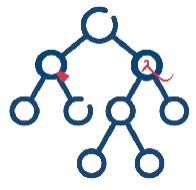
\includegraphics[height=1.0cm]{msca_logo.png}}%
    \end{center}

    \vspace{0.6cm}

    % Main title with Q logos on sides (with clickable links)
    \begin{center}
        \begin{minipage}{0.1\textwidth}
            \centering
            \href{https://quantlet.com}{
\includegraphics[height=1.1cm]{ql_logo.png}}
        \end{minipage}%
        \begin{minipage}{0.78\textwidth}
            \centering
            {\LARGE\bfseries\usebeamercolor[fg]{title}\inserttitle}

            \vspace{0.3cm}

            {\usebeamerfont{subtitle}\usebeamercolor[fg]{title}\insertsubtitle}
        \end{minipage}%
        \begin{minipage}{0.1\textwidth}
            \centering
            \href{https://quantinar.com}{
\includegraphics[height=1.1cm]{qr_logo.png}}
        \end{minipage}
    \end{center}

    \vspace{0.6cm}

    % Authors (left aligned)
    \hspace{0.5cm}{\usebeamerfont{author}\insertauthor}

    \vspace{0.3cm}

    % Institute/Affiliations (left aligned)
    \hspace{0.5cm}\begin{minipage}[t]{0.9\textwidth}
        \raggedright\small\insertinstitute
    \end{minipage}
}

%=============================================================================
% THEOREM ENVIRONMENTS
%=============================================================================
\theoremstyle{definition}
\setbeamertemplate{theorems}[numbered]
\ifdefined\atslang
\newtheorem{defn}{Definiție}
\newtheorem{thm}{Teoremă}
\newtheorem{prop}{Propoziție}
\newtheorem{rmk}{Observație}
\else
\newtheorem{defn}{Definition}
\newtheorem{thm}{Theorem}
\newtheorem{prop}{Proposition}
\newtheorem{rmk}{Remark}
\fi

%=============================================================================
% CENTRED MINIPAGE (no extra vertical space)
%=============================================================================
\newenvironment{cminipage}[1]{%
    \par\noindent\hfill\begin{minipage}{#1}\ignorespaces
}{%
    \end{minipage}\hfill\null\par
}

%=============================================================================
% CUSTOM COMMANDS
%=============================================================================
\newcommand{\E}{\mathbb{E}}
\newcommand{\Var}{\text{Var}}
\newcommand{\Cov}{\text{Cov}}
\newcommand{\Corr}{\text{Corr}}
\newcommand{\R}{\mathbb{R}}
\newcommand{\N}{\mathbb{N}}
\newcommand{\Z}{\mathbb{Z}}
\newcommand{\B}{\mathbf{B}}
\newcommand{\imark}{\textcolor{MainBlue}{\textbullet}}
\newcommand{\RMSE}{\text{RMSE}}
\newcommand{\MAE}{\text{MAE}}
\newcommand{\MAPE}{\text{MAPE}}

% Boldface vector/matrix commands (VAR, VECM, state space)
\newcommand{\bY}{\mathbf{Y}}
\newcommand{\bX}{\mathbf{X}}
\newcommand{\bA}{\mathbf{A}}
\newcommand{\bB}{\mathbf{B}}
\newcommand{\bepsilon}{\boldsymbol{\varepsilon}}
\newcommand{\bSigma}{\boldsymbol{\Sigma}}
\newcommand{\bPhi}{\boldsymbol{\Phi}}
\newcommand{\bGamma}{\boldsymbol{\Gamma}}
\newcommand{\bPi}{\boldsymbol{\Pi}}
\newcommand{\bc}{\mathbf{c}}
\newcommand{\balpha}{\boldsymbol{\alpha}}
\newcommand{\bbeta}{\boldsymbol{\beta}}
\newcommand{\bvarepsilon}{\boldsymbol{\varepsilon}}

% Seminar marks
\newcommand{\correct}{\textcolor{Forest}{\checkmark}}
\newcommand{\incorrect}{\textcolor{Crimson}{\texttimes}}


\newcommand{\qlurl}[1]{https://github.com/danpele/Advanced-Time-Series/tree/main/Quantlets/Ch_00/#1}

% Clickable citations (DOIs verified via Crossref)
\newcommand{\refHamilton}{\href{https://doi.org/10.2307/j.ctv14jx6sm}{Hamilton (1994)}}
\newcommand{\refKL}{\href{https://doi.org/10.1017/9781108164818}{Kilian and Lütkepohl (2017)}}
\newcommand{\refDK}{\href{https://doi.org/10.1093/acprof:oso/9780199641178.001.0001}{Durbin and Koopman (2012)}}
\newcommand{\refPetropoulos}{\href{https://doi.org/10.1016/j.ijforecast.2021.11.001}{Petropoulos et al.\ (2022)}}
\newcommand{\refHP}{\href{https://doi.org/10.1007/978-3-031-13584-2}{Huang and Petukhina (2022)}}
\newcommand{\refFPP}{\href{https://otexts.com/fpp3/}{Hyndman and Athanasopoulos (2021)}}
\newcommand{\refLutkepohl}{\href{https://doi.org/10.1007/978-3-540-27752-1}{Lütkepohl (2005)}}
\newcommand{\refSS}{\href{https://doi.org/10.1007/978-3-319-52452-8}{Shumway and Stoffer (2017)}}
\newcommand{\refBaltagi}{\href{https://doi.org/10.1007/978-3-030-53953-5}{Baltagi (2021)}}
\newcommand{\refAB}{\href{https://doi.org/10.1561/2200000101}{Angelopoulos and Bates (2023)}}
\newcommand{\refNW}{\href{https://doi.org/10.2307/1913610}{Newey and West (1987)}}
\newcommand{\refNWb}{\href{https://doi.org/10.2307/2297912}{Newey and West (1994)}}
\newcommand{\refAndrews}{\href{https://doi.org/10.2307/2938229}{Andrews (1991)}}
\newcommand{\refAM}{\href{https://doi.org/10.2307/2951574}{Andrews and Monahan (1992)}}
\newcommand{\refKunsch}{\href{https://doi.org/10.1214/aos/1176347265}{Künsch (1989)}}
\newcommand{\refLahiri}{\href{https://doi.org/10.1007/978-1-4757-3803-2}{Lahiri (2003)}}
\newcommand{\refPR}{\href{https://doi.org/10.1080/01621459.1994.10476870}{Politis and Romano (1994)}}
\newcommand{\refPRc}{\href{https://openlibrary.org/books/OL1551704M}{Politis and Romano (1992)}}
\newcommand{\refHolm}{\href{https://www.jstor.org/stable/4615733}{Holm (1979)}}
\newcommand{\refPW}{\href{https://doi.org/10.1081/ETC-120028836}{Politis and White (2004)}}
\newcommand{\refPPW}{\href{https://doi.org/10.1080/07474930802459016}{Patton, Politis and White (2009)}}
\newcommand{\refKV}{\href{https://doi.org/10.1017/S0266466605050565}{Kiefer and Vogelsang (2005)}}
\newcommand{\refKVB}{\href{https://doi.org/10.1111/1468-0262.00128}{Kiefer, Vogelsang and Bunzel (2000)}}
\newcommand{\refKVb}{\href{https://doi.org/10.1111/1468-0262.00366}{Kiefer and Vogelsang (2002)}}
\newcommand{\refLLSW}{\href{https://doi.org/10.1080/07350015.2018.1506926}{Lazarus et al.\ (2018)}}
\newcommand{\refLLS}{\href{https://doi.org/10.3982/ECTA15404}{Lazarus, Lewis and Stock (2021)}}
\newcommand{\refMuller}{\href{https://doi.org/10.1080/07350015.2014.931238}{Müller (2014)}}
\newcommand{\refSPJ}{\href{https://doi.org/10.1111/j.0012-9682.2008.00822.x}{Sun, Phillips and Jin (2008)}}
\newcommand{\refWhite}{\href{https://doi.org/10.1111/1468-0262.00152}{White (2000)}}
\newcommand{\refHansen}{\href{https://doi.org/10.1198/073500105000000063}{Hansen (2005)}}
\newcommand{\refRW}{\href{https://doi.org/10.1111/j.1468-0262.2005.00615.x}{Romano and Wolf (2005)}}
\newcommand{\refSTW}{\href{https://doi.org/10.1111/0022-1082.00163}{Sullivan, Timmermann and White (1999)}}
\newcommand{\refLM}{\href{https://doi.org/10.1093/rfs/3.3.431}{Lo and MacKinlay (1990)}}
\newcommand{\refHLZ}{\href{https://doi.org/10.1093/rfs/hhv059}{Harvey, Liu and Zhu (2016)}}
\newcommand{\refBH}{\href{https://doi.org/10.1111/j.2517-6161.1995.tb02031.x}{Benjamini and Hochberg (1995)}}
\newcommand{\refRosenblatt}{\href{https://doi.org/10.1073/pnas.42.1.43}{Rosenblatt (1956)}}
\newcommand{\refIbragimov}{\href{https://doi.org/10.1137/1107036}{Ibragimov (1962)}}
\newcommand{\refBrown}{\href{https://doi.org/10.1214/aoms/1177693494}{Brown (1971)}}
\newcommand{\refBillingsley}{\href{https://doi.org/10.1090/S0002-9939-1961-0126871-X}{Billingsley (1961)}}
\newcommand{\refPS}{\href{https://doi.org/10.1214/aos/1176348666}{Phillips and Solo (1992)}}
\newcommand{\refBradley}{\href{https://doi.org/10.1214/154957805100000104}{Bradley (2005)}}
\newcommand{\refCC}{\href{https://doi.org/10.1017/S0266466602181023}{Carrasco and Chen (2002)}}
\newcommand{\refMokkadem}{\href{https://doi.org/10.1016/0304-4149(88)90045-2}{Mokkadem (1988)}}
\newcommand{\refBirkhoff}{\href{https://doi.org/10.1073/pnas.17.2.656}{Birkhoff (1931)}}
\newcommand{\refWhiteH}{\href{https://doi.org/10.2307/1912934}{White (1980)}}
\newcommand{\refEfron}{\href{https://doi.org/10.1214/aos/1176344552}{Efron (1979)}}
\newcommand{\refSingh}{\href{https://doi.org/10.1214/aos/1176345636}{Singh (1981)}}
\newcommand{\refWu}{\href{https://doi.org/10.1214/aos/1176350142}{Wu (1986)}}
\newcommand{\refLiu}{\href{https://doi.org/10.1214/aos/1176351062}{Liu (1988)}}
\newcommand{\refMammen}{\href{https://doi.org/10.1214/aos/1176349025}{Mammen (1993)}}
\newcommand{\refShao}{\href{https://doi.org/10.1198/jasa.2009.tm08744}{Shao (2010)}}
\newcommand{\refBuhlmann}{\href{https://doi.org/10.2307/3318584}{Bühlmann (1997)}}
\newcommand{\refGK}{\href{https://doi.org/10.1016/j.jeconom.2003.10.030}{Gonçalves and Kilian (2004)}}
\newcommand{\refGN}{\href{https://doi.org/10.1016/0304-4076(74)90034-7}{Granger and Newbold (1974)}}
\newcommand{\refPhillips}{\href{https://doi.org/10.1016/0304-4076(86)90001-1}{Phillips (1986)}}
\newcommand{\refHH}{\href{https://doi.org/10.1086/260910}{Hansen and Hodrick (1980)}}
\newcommand{\refEH}{\href{https://doi.org/10.1111/j.1540-6261.1991.tb02674.x}{Estrella and Hardouvelis (1991)}}
\newcommand{\refVilhuber}{\href{https://doi.org/10.1162/99608f92.4f6b9e67}{Vilhuber (2020)}}
\newcommand{\refCM}{\href{https://doi.org/10.1257/jel.20171350}{Christensen and Miguel (2018)}}
\newcommand{\refCS}{\href{https://doi.org/10.1016/S0304-4076(01)00072-0}{Croushore and Stark (2001)}}

\title[Advanced Time Series Analysis and Forecasting]{Advanced Time Series Analysis and Forecasting}
\subtitle{Chapter 0: Refresher and inference for dependent data}
\author[D.T. Pele]{Daniel Traian PELE}
\institute{Bucharest University of Economic Studies\\
IDA Institute Digital Assets\\
Blockchain Research Center\\
AI4EFin Artificial Intelligence for Energy Finance\\
Romanian Academy, Institute for Economic Forecasting\\
MSCA Digital Finance}
\date{}

%=============================================================================
\providecommand{\atsapplink}[3]{\hypertarget{#2}{}\hyperlink{#1}{\beamergotobutton{#3}}}  % APPLINKS-MACROS
\providecommand{\atsappback}[2]{\begin{tikzpicture}[remember picture,overlay]\node[anchor=south east] at ([xshift=-3mm,yshift=7mm]current page.south east){\hyperlink{#1}{\beamerreturnbutton{#2}}};\end{tikzpicture}}  % APPLINKS-MACROS
\providecommand{\atschlink}[2]{\href{#1}{#2}}  % APPLINKS-MACROS
\providecommand{\atschlinkt}[2]{\href{#1}{\usebeamercolor[fg]{frametitle}#2}}  % APPLINKS-MACROS
\begin{document}
%=============================================================================

{
\setbeamertemplate{headline}{}
\setbeamertemplate{footline}{}
\begin{frame}[noframenumbering]
    \titlepage
\end{frame}
}
% BEGIN-ACRONYMS (generat de latex/acronyms.py; nu editati manual)
\begin{frame}{Acronyms used in this material (1/2)}
\setbeamertemplate{itemize/enumerate body begin}{\footnotesize}
\begin{columns}[T]
\begin{column}{0.49\textwidth}
\begin{itemize}\setlength{\itemsep}{0pt}
    \item \textbf{ACF}: Autocorrelation Function
    \item \textbf{AI}: Artificial Intelligence
    \item \textbf{ALFRED}: ArchivaL Federal Reserve Economic Data
    \item \textbf{AR}: AutoRegressive (model)
    \item \textbf{ARDL}: AutoRegressive Distributed Lag (model)
    \item \textbf{ARIMA}: AutoRegressive Integrated Moving Average (model)
    \item \textbf{ARMA}: AutoRegressive Moving Average (model)
    \item \textbf{ASDS}: Statistică aplicată și data science (the Master's programme Applied Statistics and Data Science)
    \item \textbf{ASE}: Academia de Studii Economice din București (the Bucharest University of Economic Studies)
    \item \textbf{ATS}: Advanced Time Series Analysis and Forecasting
    \item \textbf{BET}: Bucharest Exchange Trading (index)
    \item \textbf{BNR}: Banca Națională a României (the National Bank of Romania)
\end{itemize}
\end{column}
\begin{column}{0.49\textwidth}
\begin{itemize}\setlength{\itemsep}{0pt}
    \item \textbf{BVAR}: Bayesian Vector AutoRegression
    \item \textbf{CBB}: Circular Block Bootstrap
    \item \textbf{CLT}: Central Limit Theorem
    \item \textbf{CPI}: Consumer Price Index
    \item \textbf{DGP}: Data-Generating Process
    \item \textbf{ECB}: European Central Bank
    \item \textbf{ECTS}: European Credit Transfer and Accumulation System
    \item \textbf{EOD}: End Of Day (daily closing data)
    \item \textbf{EODHD}: EOD Historical Data (market-data provider)
    \item \textbf{ES}: Expected Shortfall
    \item \textbf{EU}: European Union
    \item \textbf{EWC}: Equal-Weighted Cosine (estimator)
    \item \textbf{FDR}: False Discovery Rate
    \item \textbf{FM-OLS}: Fully Modified Ordinary Least Squares
\end{itemize}
\end{column}
\end{columns}
\end{frame}
\begin{frame}{Acronyms used in this material (2/2)}
\setbeamertemplate{itemize/enumerate body begin}{\footnotesize}
\begin{columns}[T]
\begin{column}{0.49\textwidth}
\begin{itemize}\setlength{\itemsep}{0pt}
    \item \textbf{FRED}: Federal Reserve Economic Data
    \item \textbf{FWER}: Family-Wise Error Rate
    \item \textbf{GARCH}: Generalised AutoRegressive Conditional Heteroskedasticity
    \item \textbf{GDP}: Gross Domestic Product
    \item \textbf{HAC}: Heteroskedasticity and Autocorrelation Consistent (standard errors)
    \item \textbf{HAR}: Heterogeneous AutoRegressive (model)
    \item \textbf{HICP}: Harmonised Index of Consumer Prices
    \item \textbf{INS}: Institutul Național de Statistică (the National Institute of Statistics (Romania))
    \item \textbf{KPSS}: Kwiatkowski–Phillips–Schmidt–Shin (test)
    \item \textbf{LLN}: Law of Large Numbers
    \item \textbf{LLSW}: Lazarus, Lewis, Stock and Watson (2018)
    \item \textbf{MA}: Moving Average
\end{itemize}
\end{column}
\begin{column}{0.49\textwidth}
\begin{itemize}\setlength{\itemsep}{0pt}
    \item \textbf{MBB}: Moving-Block Bootstrap
    \item \textbf{MDS}: Martingale Difference Sequence
    \item \textbf{MFM}: Modelling Financial Markets
    \item \textbf{MSE}: Mean Squared Error
    \item \textbf{NW}: Newey–West (standard errors)
    \item \textbf{NW-A}: Newey–West with the Andrews (1991) bandwidth
    \item \textbf{OLS}: Ordinary Least Squares
    \item \textbf{QR}: Quick Response (code)
    \item \textbf{QS}: Quadratic Spectral (kernel)
    \item \textbf{SARIMA}: Seasonal ARIMA (model)
    \item \textbf{SPA}: Superior Predictive Ability (test)
    \item \textbf{TSA}: Time Series Analysis
    \item \textbf{US}: United States
    \item \textbf{VAR}: Vector AutoRegression
    \item \textbf{VECM}: Vector Error Correction Model
\end{itemize}
\end{column}
\end{columns}
\end{frame}
% END-ACRONYMS

%=============================================================================
\section{Course organisation}
%=============================================================================

\begin{frame}{The course at a glance}
\itemsize{\footnotesize}
\begin{columns}[T]
\begin{column}{0.56\textwidth}
\begin{itemize}
    \item \textbf{Programme}
    \begin{itemize}
        \item Master's programme Applied Statistics and Data Science (ASDS), year 1, semester 2
        \item Faculty of Cybernetics, Statistics and Economic Informatics, ASE Bucharest
        \item 7 ECTS credits; 2 hours of lecture and 2 hours of seminar a week; academic year 2026/2027
    \end{itemize}
    \item \textbf{Lecturer}
    \begin{itemize}
        \item Prof.\ Daniel Traian Pele, \href{mailto:danpele@ase.ro}{danpele@ase.ro}
    \end{itemize}
    \item \textbf{Course website}
    \begin{itemize}
        \item \href{https://danpele.github.io/Advanced-Time-Series/}{danpele.github.io/Advanced-Time-Series}
        \item slides, seminars, notebooks, Quantlets and the graded quizzes
    \end{itemize}
\end{itemize}
\end{column}
\begin{column}{0.40\textwidth}
\centering
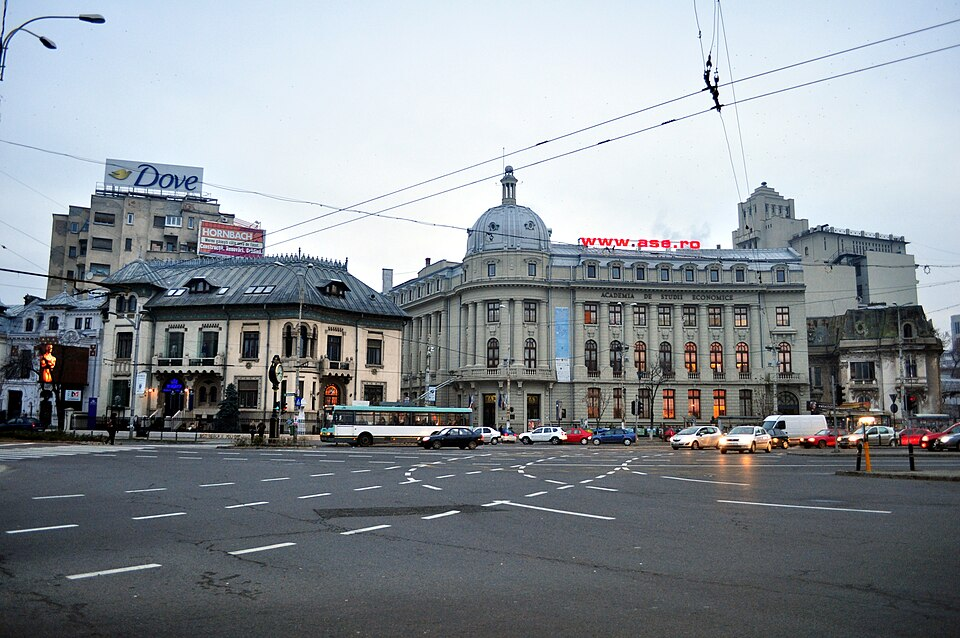
\includegraphics[height=0.46\textheight]{ch0_ase_2014.jpg}\\[1mm]
\imgcap{The Bucharest University of Economic Studies (ASE)}
\imgcredit{https://commons.wikimedia.org/wiki/File:Bucharest_-_Academie_de_Studii_Economice_01.jpg}{Photo: Joe Mabel (2014); CC BY 3.0; Wikimedia Commons}
\end{column}
\end{columns}
\end{frame}

\begin{frame}{Position in the curriculum}
\itemsize{\footnotesize}
\begin{itemize}
    \item \textbf{Before}: \href{https://danpele.github.io/Time-Series-Analysis/}{Time Series Analysis} (TSA, bachelor), Chapters 0--10 of TSA
    \begin{itemize}
        \item ARMA, ARIMA and unit roots, SARIMA, GARCH, VAR and Granger causality, cointegration and VECM, long memory, machine learning, state space models
        \item assumed known: this course starts from them and does not repeat them
    \end{itemize}
    \item \textbf{This course}: ATS, master, year 1, semester 2
    \begin{itemize}
        \item methodology for forecasting, identification and inference with dependent data
        \item macroeconomic (Romanian and EU), energy, climate and financial series
    \end{itemize}
    \item \textbf{After}: \href{https://danpele.github.io/MFM/}{Modelling Financial Markets} (MFM, master, year 2, semester 1)
    \begin{itemize}
        \item the same methods applied to market risk, portfolios, microstructure and digital assets
    \end{itemize}
\end{itemize}
\end{frame}

\begin{frame}{Evaluation}
\itemsize{\small}
\begin{itemize}
    \item \textbf{Team project and individual oral defence: 70\%}
    \begin{itemize}
        \item proposal and pre-registration (team): 5\%
        \item replication and extension: repository, report, AI\_USE.md and AI\_ERRORS.md (team): 15\%
        \item individual oral defence: 50\%
    \end{itemize}
    \item \textbf{Chapter quizzes: 20\%}
    \begin{itemize}
        \item online, on the course website, with the ASE Google account
    \end{itemize}
    \item \textbf{Attendance: 10\%}
    \begin{itemize}
        \item recorded with the attendance form or the QR code
    \end{itemize}
    \item There is no written exam
\end{itemize}
\end{frame}

\begin{frame}{Textbooks}
\itemsize{\small}
\begin{itemize}
    \item \textbf{Main references}
    \begin{itemize}
        \item \refHamilton: the theory of linear time series, unit roots and VAR
        \item \refKL: structural VAR analysis and identification
        \item \refDK: state space methods
        \item \refPetropoulos: forecasting theory and practice, open access
    \end{itemize}
    \item \textbf{Bridge from the bachelor course}
    \begin{itemize}
        \item \refHP; \refFPP
    \end{itemize}
    \item \textbf{Specialised}
    \begin{itemize}
        \item \refLutkepohl; \refSS; \refBaltagi; \refAB; for this chapter also \refLahiri
        \item each chapter adds its landmark papers as case studies
    \end{itemize}
\end{itemize}
\end{frame}

\begin{frame}{Course map (1/2)}
\begin{center}
\footnotesize
\begin{tabular}{rl}
\toprule
\textbf{Ch.} & \textbf{Topic} \\
\midrule
0 & Refresher and inference for dependent data \\
1 & Forecast evaluation, scoring rules and combination \\
2 & Structural breaks and nonlinear models \\
3 & Structural VAR and local projections \\
4 & Cointegration revisited: VECM, ARDL and panel data \\
5 & Bayesian VAR, factor models and nowcasting \\
6 & State space models and Bayesian filtering \\
7 & Regime-switching models \\
8 & Advanced volatility modelling: realised measures, HAR and multivariate GARCH \\
\bottomrule
\end{tabular}
\end{center}
\end{frame}

\begin{frame}{Course map (2/2)}
\begin{center}
\footnotesize
\begin{tabular}{rl}
\toprule
\textbf{Ch.} & \textbf{Topic} \\
\midrule
9 & VaR, ES and backtesting: elicitability, scoring and model risk \\
10 & Long memory and rough volatility \\
11 & Spectral and wavelet analysis \\
12 & Machine learning and deep learning for time series \\
13 & Foundation models and conformal prediction \\
14 & Causal inference for time series \\
15 & Review and project defence \\
16 & Explosive roots and bubbles (self-study) \\
\bottomrule
\end{tabular}
\end{center}
\end{frame}

\begin{frame}{Lectures and seminars}
\itemsize{\footnotesize}
\begin{itemize}
    \item \textbf{Lectures}
    \begin{itemize}
        \item one chapter a week, built around landmark papers replicated on our data
        \item each lecture ends with a section on AI for scientific discovery
    \end{itemize}
    \item \textbf{Seminars}: each seminar comes \emph{before} its lecture and opens with the notions it needs
    \begin{itemize}
        \item Part A: derivations; Part B: estimation and inference on data, each exercise closing with an interpretation question; Part C: open problems that can seed the project
        \item [Solved] exercises with full solutions and [Proposed] exercises discussed in class
        \item every seminar includes the critique of an answer given by an AI tool
    \end{itemize}
    \item Seminars are practice and are not graded; the solutions of the [Proposed] exercises are discussed in class
\end{itemize}
\end{frame}

\begin{frame}{The team project}
\itemsize{\footnotesize}
\begin{itemize}
    \item \textbf{Teams of up to 3 students}
    \begin{itemize}
        \item replicate a landmark paper of the course, or another paper approved by the lecturer
        \item extend it with the methods of the course, preferably on Romanian or EU data
    \end{itemize}
    \item \textbf{Stages}
    \begin{itemize}
        \item Stage 1: research question, data and an evaluation design fixed before any estimation (pre-registration)
        \item Stage 2: replication, extension and a GitHub repository that reproduces every number (Colab)
        \item Stage 3: presentation and individual oral defence
    \end{itemize}
    \item Inference that is valid for dependent data (this chapter) is part of every project
    \item The project can be written and defended in Romanian or in English
\end{itemize}
\end{frame}

\begin{frame}{AI policy}
\itemsize{\small}
\begin{itemize}
    \item \textbf{Allowed and declared}
    \begin{itemize}
        \item AI\_USE.md: tool, purpose, prompts, what was kept and what was changed
        \item AI\_ERRORS.md: at least three errors of AI tools caught by the team, and how each was detected
        \item undeclared use counts as plagiarism
    \end{itemize}
    \item \textbf{Checked}
    \begin{itemize}
        \item every reference against its DOI, every number against the data and the code
    \end{itemize}
    \item \textbf{Oral defence without AI}
    \begin{itemize}
        \item each member explains the methods, the code and the results
    \end{itemize}
\end{itemize}
\end{frame}

\begin{frame}{Materials and tools}
\itemsize{\small}
\begin{itemize}
    \item \textbf{For every chapter}
    \begin{itemize}
        \item lecture and seminar slides in English and Romanian
        \item lecture and seminar notebooks in English, runnable in Google Colab
        \item a Quantlet with the code of every chart, and a quiz
    \end{itemize}
    \item \textbf{Data}
    \begin{itemize}
        \item daily market data from EODHD (EOD Historical Data), saved in the course repository
        \item public macroeconomic data: INS, BNR, Eurostat, the ECB and FRED
    \end{itemize}
    \item \textbf{Software}
    \begin{itemize}
        \item Python: statsmodels, arch, linearmodels, scikit-learn, PyTorch
    \end{itemize}
\end{itemize}
\end{frame}


%=============================================================================
\section{Chapter 0: the plan}
%=============================================================================

\begin{frame}{Learning outcomes}
\itemsize{\small}
\begin{itemize}
    \item State the limit theorems behind every standard error used with time series: ergodic LLN, martingale-difference and mixing CLT
    \item Derive the long-run variance and its consequences for $t$-tests and confidence intervals
    \item Choose and defend a HAC estimator: kernel, bandwidth, critical values (standard or fixed-$b$)
    \item Use block bootstraps (moving, circular, stationary) and know when the wild bootstrap is not enough
    \item Measure size distortions by Monte Carlo and control data snooping
    \item Build a replication package that reproduces every number of a project
\end{itemize}
\end{frame}

\begin{frame}{Data used in this chapter}
\itemsize{\footnotesize}
\begin{center}
\scriptsize
\begin{tabular}{p{3.0cm}p{5.0cm}p{2.6cm}p{1.6cm}}
\toprule
\textbf{Series} & \textbf{Definition} & \textbf{Period} & \textbf{Source} \\
\midrule
Romanian inflation & HICP, annual rate of change, \%, monthly & January 2006 -- August 2026 & Eurostat \\
Romanian real GDP & chain-linked volumes, seasonally adjusted; growth q/q, \% & 2000Q1 -- 2026Q2 & Eurostat \\
EUR/RON & BNR reference rate; daily log change, \% & 5 July 2005 -- 18 September 2026 & BNR \\
S\&P 500, BET & daily log returns and squared returns, \% & 2000 -- 18 September 2026 & EODHD \\
US macro & real GDP; 10-year and 3-month Treasury yields & 1962 -- 2026 & FRED \\
\bottomrule
\end{tabular}
\end{center}
\begin{itemize}
    \item Daily series on their own trading calendars; Eurostat and FRED series read online at the build date
    \item HICP: harmonised index of consumer prices; the BNR target is defined on the national CPI, close to the HICP
\end{itemize}
\end{frame}

\begin{frame}{Where the data come from}
\itemsize{\footnotesize}
\begin{columns}[T]
\begin{column}{0.48\textwidth}
\centering

\includegraphics[height=0.40\textheight]{ch0_bnr_palace_2015.jpg}\\[1mm]
\imgcap{The National Bank of Romania (BNR), Bucharest: reference rates and the inflation target}
\imgcredit{https://commons.wikimedia.org/wiki/File:Bucharest_-_BNR_Palace_(19644434340).jpg}{Photo: Ștefan Jurcă (2015); CC BY 2.0; Wikimedia Commons}
\end{column}
\begin{column}{0.48\textwidth}
\centering

\includegraphics[height=0.40\textheight]{ch0_eccles_2011.jpg}\\[1mm]
\imgcap{The Eccles Building, Washington: the Federal Reserve Board; FRED is run by the St.\ Louis Fed}
\imgcredit{https://commons.wikimedia.org/wiki/File:Eccles_Building_(26088200676).jpg}{Photo: Federal Reserve (2011); public domain; Wikimedia Commons}
\end{column}
\end{columns}\begin{itemize}
    \item A central bank publishes the series we test: the inflation target of the BNR is 2.5\% $\pm$ 1 pp since 2013 (the AI mini-case at the end)
\end{itemize}
\end{frame}

\begin{frame}{Notation (1/2)}
\itemsize{\small}
\begin{itemize}
    \item $\{x_t\}$, $t = 1, \dots, T$: a weakly stationary series observed over $T$ periods
    \begin{itemize}
        \item $\mu = E x_t$: its mean; $\gamma_j = \Cov(x_t, x_{t-j})$: the autocovariance at lag $j$, the same for every $t$
        \item $\gamma_0 = \Var(x_t)$; $\rho_j = \gamma_j/\gamma_0 \in [-1, 1]$: the autocorrelation at lag $j$
    \end{itemize}
    \item Sample counterparts (a hat marks an estimated value)
    \begin{itemize}
        \item sample mean $\bar{x} = T^{-1}\sum_{t=1}^{T} x_t$
        \item sample autocovariance $\hat\gamma_j = T^{-1}\sum_{t=j+1}^{T}(x_t - \bar x)(x_{t-j} - \bar x)$
        \item $\hat\gamma_j$ averages the products of deviations from the mean that lie $j$ periods apart
    \end{itemize}
    \item Long-run variance $\Omega = \sum_{j=-\infty}^{\infty}\gamma_j = 2\pi f(0)$
    \begin{itemize}
        \item the sum of all autocovariances ($\gamma_{-j} = \gamma_j$); it governs the precision of $\bar x$ (next section)
        \item $f(\omega)$: the spectral density at frequency $\omega$; $f(0)$ measures the variance of the slow, long-run movements
    \end{itemize}
\end{itemize}
\end{frame}

\begin{frame}{Notation (2/2)}
\itemsize{\small}
\begin{itemize}
    \item Kernel $k(\cdot)$: a weight function with $k(0) = 1$; lag $j$ receives the weight $k(j/S)$
    \begin{itemize}
        \item bandwidth $S$: the scale of the weights; lags much longer than $S$ get (almost) zero weight
        \item Newey--West: $L = S - 1$ lags for the Bartlett kernel; $b = S/T$: the bandwidth as a share of the sample
    \end{itemize}
    \item Size of a test: the probability of rejecting a true $H_0$
    \begin{itemize}
        \item nominal level $5\%$ unless stated; a test over-rejects when its actual size exceeds the nominal level
    \end{itemize}
    \item HAC: heteroskedasticity and autocorrelation consistent (an estimator of $\Omega$)
    \begin{itemize}
        \item HAR: heteroskedasticity and autocorrelation robust (the test built on a HAC estimator)
    \end{itemize}
\end{itemize}
\end{frame}


%=============================================================================
\section{A refresher map of TSA}
%=============================================================================

\begin{frame}{Prior knowledge from TSA (bachelor)}
\itemsize{\footnotesize}
\begin{center}
\scriptsize
\begin{tabular}{p{3.2cm}p{2.6cm}p{7.2cm}}
\toprule
\textbf{Topic} & \textbf{TSA} & \textbf{Used in ATS for} \\
\midrule
Stationarity, ACF, Wold & \atschlink{https://danpele.github.io/Time-Series-Analysis/EN/Courses/chapter1_stochastic_processes_stationarity.pdf}{TSA, Chapter 1} & long-run variance, HAC, bootstrap (this chapter) \\
ARMA & \atschlink{https://danpele.github.io/Time-Series-Analysis/EN/Courses/chapter2_arma_models.pdf}{TSA, Chapter 2} & benchmarks, Monte Carlo designs, sieve bootstrap \\
Unit roots, ARIMA & \atschlink{https://danpele.github.io/Time-Series-Analysis/EN/Courses/chapter3_unit_roots_arima_models.pdf}{TSA, Chapter 3} & nonstandard asymptotics, spurious regression, \atschlink{https://danpele.github.io/Advanced-Time-Series/EN/Courses/chapter2_structural_breaks_nonlinear_models.pdf}{Chapters 2}, \atschlink{https://danpele.github.io/Advanced-Time-Series/EN/Courses/chapter4_cointegration_vecm_ardl_panel.pdf}{4}, \atschlink{https://danpele.github.io/Advanced-Time-Series/EN/Courses/chapter16_explosive_roots_bubbles.pdf}{16} \\
GARCH & \atschlink{https://danpele.github.io/Time-Series-Analysis/EN/Courses/chapter5_conditional_volatility_garch.pdf}{TSA, Chapter 5} & martingale differences, \atschlink{https://danpele.github.io/Advanced-Time-Series/EN/Courses/chapter8_advanced_volatility.pdf}{Chapters 8}--\atschlink{https://danpele.github.io/Advanced-Time-Series/EN/Courses/chapter9_var_es_backtesting.pdf}{9} \\
VAR, Granger & \atschlink{https://danpele.github.io/Time-Series-Analysis/EN/Courses/chapter6_var_models_granger_causality.pdf}{TSA, Chapter 6} & structural VAR, local projections, BVAR (\atschlink{https://danpele.github.io/Advanced-Time-Series/EN/Courses/chapter3_structural_var_local_projections.pdf}{Chapters 3}, \atschlink{https://danpele.github.io/Advanced-Time-Series/EN/Courses/chapter5_bvar_factor_models_nowcasting.pdf}{5}) \\
Cointegration, VECM & \atschlink{https://danpele.github.io/Time-Series-Analysis/EN/Courses/chapter7_cointegration_vecm.pdf}{TSA, Chapter 7} & ARDL, panel cointegration (\atschlink{https://danpele.github.io/Advanced-Time-Series/EN/Courses/chapter4_cointegration_vecm_ardl_panel.pdf}{Chapter 4}) \\
Long memory & \atschlink{https://danpele.github.io/Time-Series-Analysis/EN/Courses/chapter8_long_memory_arfima.pdf}{TSA, Chapter 8} & local Whittle, rough volatility (\atschlink{https://danpele.github.io/Advanced-Time-Series/EN/Courses/chapter10_long_memory_rough_volatility.pdf}{Chapter 10}) \\
State space, Markov switching & \atschlink{https://danpele.github.io/Time-Series-Analysis/EN/Courses/chapter10_state_space_kalman_markov_switching.pdf}{TSA, Chapter 10} & filtering and regimes (\atschlink{https://danpele.github.io/Advanced-Time-Series/EN/Courses/chapter6_state_space_models_bayesian_filtering.pdf}{Chapters 6}, \atschlink{https://danpele.github.io/Advanced-Time-Series/EN/Courses/chapter7_regime_switching_models.pdf}{7}) \\
\bottomrule
\end{tabular}
\end{center}
\begin{itemize}
    \item Slides of the bachelor course: \atschlink{https://danpele.github.io/Time-Series-Analysis/EN/Courses/chapter1_stochastic_processes_stationarity.pdf}{TSA, Chapter 1} to \atschlink{https://danpele.github.io/Time-Series-Analysis/EN/Courses/chapter10_state_space_kalman_markov_switching.pdf}{TSA, Chapter 10}; each ATS chapter links to the TSA chapter it extends
\end{itemize}
\end{frame}

\begin{frame}{Stationarity and the Wold representation}
\itemsize{\small}
\begin{itemize}
    \item \atschlink{https://danpele.github.io/Time-Series-Analysis/EN/Courses/chapter1_stochastic_processes_stationarity.pdf}{TSA, Chapter 1}. Weak stationarity: constant mean and $\gamma_j$ depending only on $j$
    \begin{itemize}
        \item strict stationarity: all finite-dimensional distributions are invariant to a shift in time
        \item neither implies the other without moment conditions: Cauchy i.i.d.\ is strictly but not weakly stationary (no variance)
    \end{itemize}
    \item Wold theorem \refHamilton: every weakly stationary, purely nondeterministic series is a weighted sum of past innovations
    \begin{itemize}
        \item $x_t - \mu = \sum_{j\ge 0}\psi_j\varepsilon_{t-j}$, $\quad \psi_0 = 1$, $\quad \sum_j\psi_j^2 < \infty$
        \item $\varepsilon_t$: white noise with variance $\sigma^2$, the one-step forecast error; $\psi_j$: the effect of a shock after $j$ periods
        \item $\varepsilon_t$ is uncorrelated, not necessarily independent: GARCH innovations are Wold innovations
    \end{itemize}
    \item Hence white noise is not enough for i.i.d.-based inference on squares or on extremes
    \begin{itemize}
        \item In this chapter: $\Omega = \sigma^2 \big(\sum_j \psi_j\big)^2$; $\sum_j\psi_j$ is the cumulative (long-run) effect of a shock, so $\Omega$ is the variance of the permanent component
    \end{itemize}
\end{itemize}
\end{frame}

\begin{frame}{ARMA and unit roots (1/2)}
\itemsize{\small}
\begin{itemize}
    \item \atschlink{https://danpele.github.io/Time-Series-Analysis/EN/Courses/chapter2_arma_models.pdf}{TSA, Chapter 2}. ARMA$(p,q)$: $\phi(L)x_t = \theta(L)\varepsilon_t$
    \begin{itemize}
        \item $L$: the lag operator, $Lx_t = x_{t-1}$; $\phi(L) = 1 - \phi_1L - \dots - \phi_pL^p$; $\theta(L) = 1 + \theta_1L + \dots + \theta_qL^q$
        \item stationary if the roots of $\phi(z)$ lie outside the unit circle; invertible if those of $\theta(z)$ do
    \end{itemize}
    \item Long-run variance in closed form: $\Omega = \sigma^2\,\theta(1)^2/\phi(1)^2$
    \begin{itemize}
        \item $\phi(1) = 1 - \sum_i\phi_i$ and $\theta(1) = 1 + \sum_i\theta_i$: the two polynomials evaluated at $z = 1$
        \item AR(1): $\Omega = \sigma^2/(1-\phi)^2$; the closer $\phi(1)$ is to 0 (more persistence), the larger $\Omega$
    \end{itemize}
\end{itemize}
\end{frame}

\begin{frame}{ARMA and unit roots (2/2)}
\itemsize{\small}
\begin{itemize}
    \item \atschlink{https://danpele.github.io/Time-Series-Analysis/EN/Courses/chapter3_unit_roots_arima_models.pdf}{TSA, Chapter 3}. Unit root, $\phi(1) = 0$: $\Omega = \infty$ and the mean is not defined
    \begin{itemize}
        \item the $t$-statistic has a nonstandard (Dickey--Fuller) limit
    \end{itemize}
    \item Spurious regression: one random walk regressed on an independent one
    \begin{itemize}
        \item $|t| > 2$ in 76 of 100 regressions in \refGN
        \item the $t$-statistic diverges at rate $\sqrt{T}$ \refPhillips
        \item no HAC estimator repairs a spurious regression (Seminar 0, B5)
    \end{itemize}
    \item Near unit roots ($\phi$ close to 1) are the hard case of this chapter
    \begin{itemize}
        \item every HAC method over-rejects there (Monte Carlo section)
    \end{itemize}
\end{itemize}
\end{frame}

\begin{frame}{GARCH, VAR, cointegration, state space}
\itemsize{\footnotesize}
\begin{itemize}
    \item GARCH (\atschlink{https://danpele.github.io/Time-Series-Analysis/EN/Courses/chapter5_conditional_volatility_garch.pdf}{TSA, Chapter 5}): $r_t = \sigma_t z_t$ is a martingale difference; $r_t^2$ is an ARMA(1,1) with strong, slowly decaying autocorrelation
    \begin{itemize}
        \item $r_t$: the return; $\sigma_t$: its conditional volatility; $z_t$: i.i.d.\ with mean 0 and variance 1
        \item Means of returns: HAC barely matters; means of squared returns (variances, risk premia): HAC matters a lot
    \end{itemize}
    \item VAR (\atschlink{https://danpele.github.io/Time-Series-Analysis/EN/Courses/chapter6_var_models_granger_causality.pdf}{TSA, Chapter 6}): Granger causality tests are Wald tests; with heteroskedastic errors they need robust covariances
    \begin{itemize}
        \item Local projections (\atschlink{https://danpele.github.io/Advanced-Time-Series/EN/Courses/chapter3_structural_var_local_projections.pdf}{Chapter 3}) have serially correlated errors by construction: HAC is part of the method
    \end{itemize}
    \item Cointegration (\atschlink{https://danpele.github.io/Time-Series-Analysis/EN/Courses/chapter7_cointegration_vecm.pdf}{TSA, Chapter 7}): long-run relations; the long-run variance reappears in FM-OLS and in the KPSS statistic
    \item State space (\atschlink{https://danpele.github.io/Time-Series-Analysis/EN/Courses/chapter10_state_space_kalman_markov_switching.pdf}{TSA, Chapter 10}): the Kalman filter gives the Gaussian likelihood; its standard errors still need the sandwich form under misspecification
\end{itemize}
\end{frame}

\begin{frame}{The series of this chapter}
\itemsize{\footnotesize}
\begin{center}
    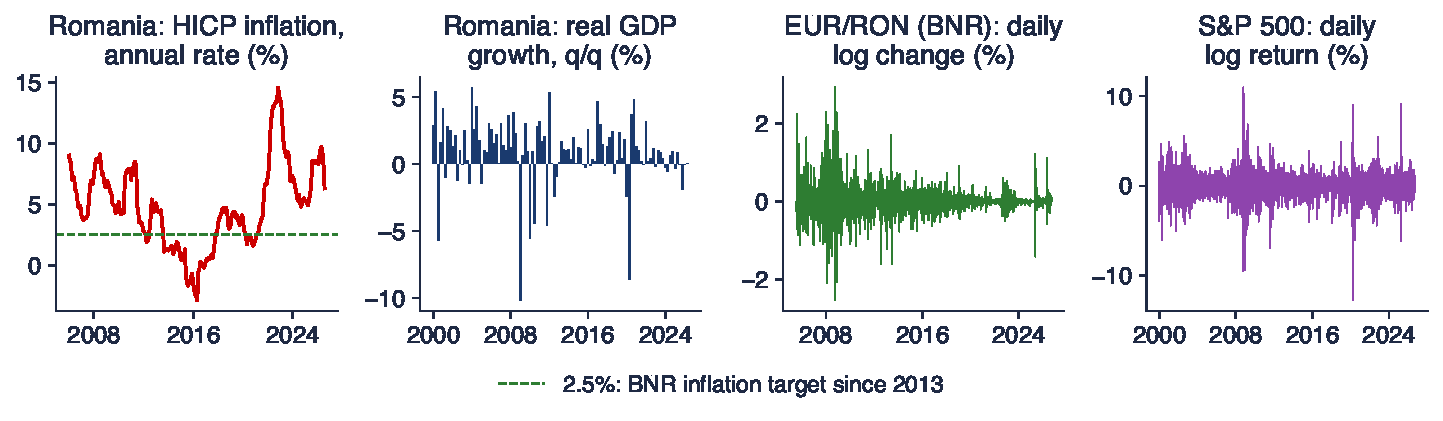
\includegraphics[width=0.97\textwidth,height=0.56\textheight,keepaspectratio]{ats_ch0_data_dashboard.pdf}
\end{center}
\vspace{-0.25cm}
\begin{itemize}
    \item Romanian HICP inflation, January 2006 -- August 2026: from $\ensuremath{-}2.9\%$ (May 2016) to $14.6\%$ (November 2022); last value $6.3\%$
    \item Romanian GDP growth: 106 quarters, minimum $\ensuremath{-}10.2\%$ in 2009Q1; daily: 5\,352 EUR/RON and 6\,714 S\&P 500 observations
\end{itemize}
\quantlet{ATS\_ch0\_dependence\_data}{\qlurl{ATS_ch0_dependence_data}}
\end{frame}

\begin{frame}{Interpreting the four series}
\itemsize{\small}
\begin{itemize}
    \item Inflation moves in long swings: years above and years below the 2.5\% line
    \begin{itemize}
        \item Each monthly value shares eleven months with the previous one (annual rate): overlap adds to persistence
    \end{itemize}
    \item GDP growth looks close to white noise, apart from two crisis quarters
    \begin{itemize}
        \item With $T = 106$, two outliers dominate the sample variance
    \end{itemize}
    \item EUR/RON and the S\&P 500: volatility clusters (calm years, crisis bursts): dependence in the second moment
    \item What do you think? Which of the four series has the largest long-run variance relative to its variance?
    \begin{itemize}
        \item Answer: inflation, the most persistent series; the ratios are on the slide ``Interpreting the autocorrelations''
    \end{itemize}
\end{itemize}
\end{frame}

\begin{frame}{Autocorrelation in six series}
\itemsize{\footnotesize}
\begin{center}
    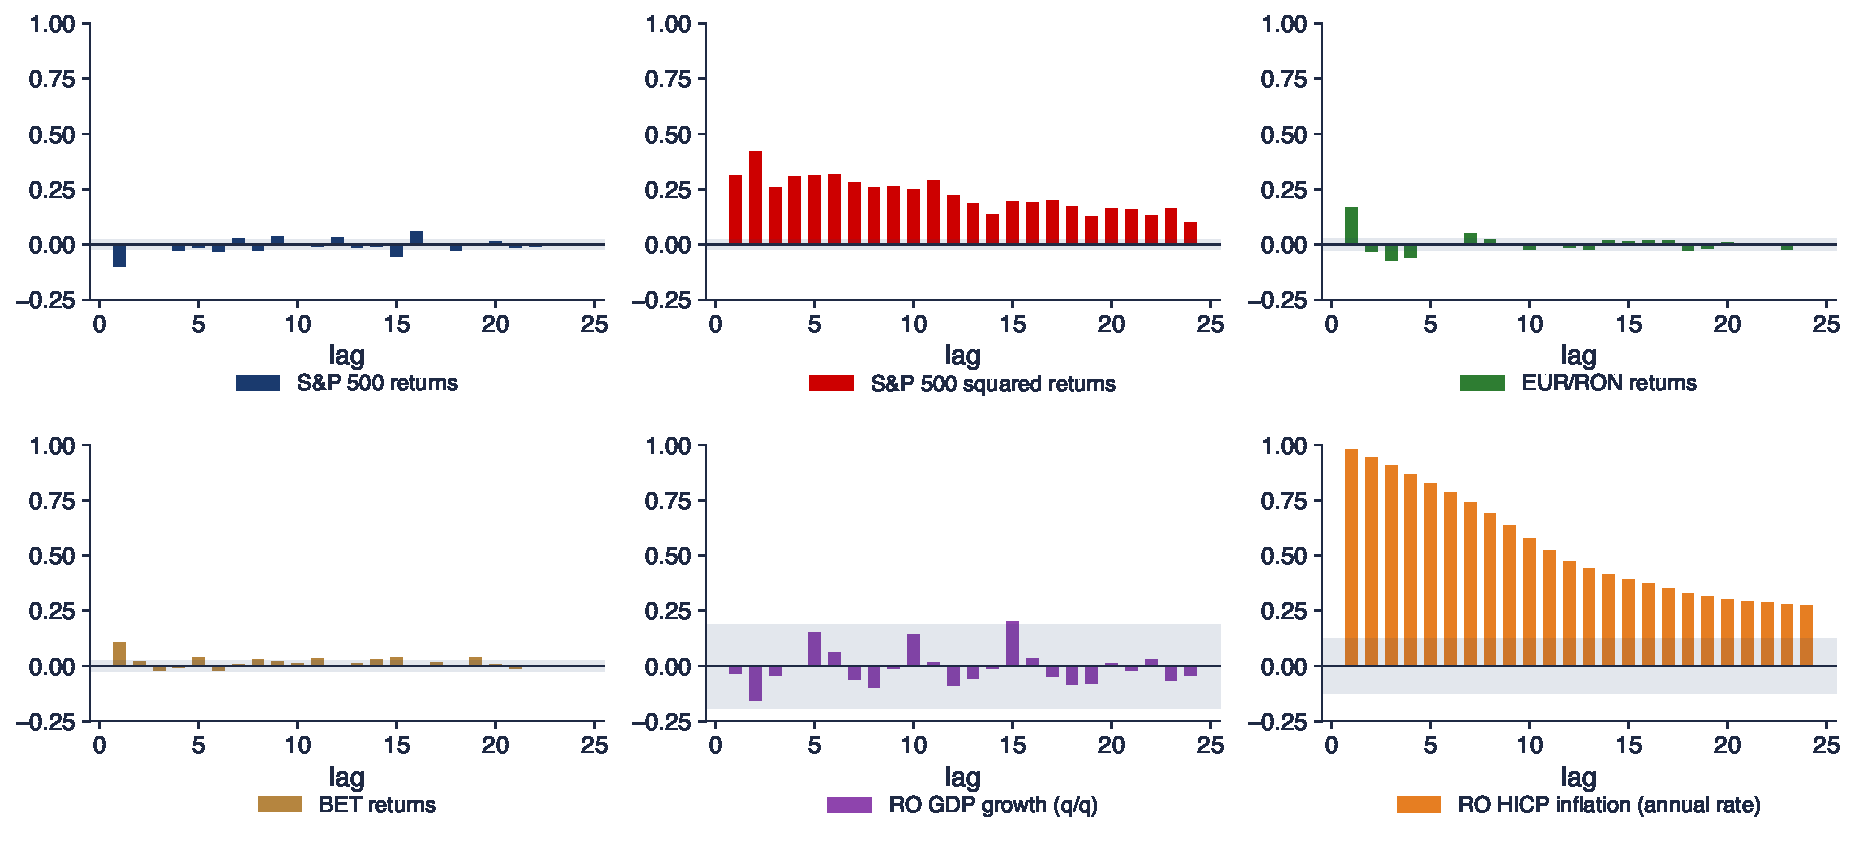
\includegraphics[width=0.97\textwidth,height=0.55\textheight,keepaspectratio]{ats_ch0_acf_panel.pdf}
\end{center}
\vspace{-0.25cm}
\begin{itemize}
    \item Sample ACF, lags 1--24, with the $\pm 1.96/\sqrt{T}$ band of the i.i.d.\ hypothesis (shaded)
    \item $\hat\rho_1$: S\&P 500 $\ensuremath{-}0.10$, squared $0.31$, EUR/RON $0.17$, BET $0.11$, GDP $\ensuremath{-}0.03$, inflation $0.98$
\end{itemize}
\quantlet{ATS\_ch0\_dependence\_data}{\qlurl{ATS_ch0_dependence_data}}
\end{frame}

\begin{frame}{Interpreting the autocorrelations}
\itemsize{\small}
\begin{itemize}
    \item S\&P 500 returns: small negative $\hat\rho_1$; squared returns: all 24 lags above the band, $\hat\rho_{12} = 0.22$
    \begin{itemize}
        \item Long-run variance over variance (Andrews bandwidth): $0.8$ for returns, $5.7$ for squared returns
    \end{itemize}
    \item BET and EUR/RON: positive $\hat\rho_1$ (thin trading, central-bank smoothing of the reference rate)
    \begin{itemize}
        \item Ratios $1.2$ and $1.1$: modest, but enough to move a borderline $t$-statistic
    \end{itemize}
    \item Inflation: $\hat\rho_1 = 0.98$ and a ratio of $27.0$: a naive standard error is about five times too small
    \item The rest of the chapter: what these ratios mean, how to estimate them, and when the estimates fail
\end{itemize}
\end{frame}

\begin{frame}{Recap: the refresher map}
\itemsize{\small}
\begin{itemize}
    \item TSA gave the models; ATS needs the inference that goes with dependent data
    \item White noise is not independence: GARCH returns are uncorrelated, their squares are not
    \item The long-run variance $\Omega = \sigma^2\theta(1)^2/\phi(1)^2$ links ARMA models to the precision of a sample mean
    \item In our data the dependence ranges from negligible (GDP growth) to extreme (inflation, squared returns)
\end{itemize}
\end{frame}


%=============================================================================
\section{Asymptotics for dependent data}
%=============================================================================

\begin{frame}{The variance of a mean under dependence}
\itemsize{\small}
\begin{itemize}
    \item Exact, for any weakly stationary series: the variance of the scaled mean adds up the covariances of all pairs of observations
    \begin{itemize}
        \item $\Var(\sqrt{T}\,\bar x) = \dfrac{1}{T}\sum_{t=1}^{T}\sum_{s=1}^{T}\gamma_{t-s} = \sum_{|j| < T}\Big(1 - \dfrac{|j|}{T}\Big)\gamma_j$
        \item $\gamma_{t-s}$: the covariance of $x_t$ and $x_s$; $T - |j|$ pairs lie at distance $j$, hence the weight $1 - |j|/T$
    \end{itemize}
    \item If $\sum_j |\gamma_j| < \infty$, the weights tend to 1 (dominated convergence):
    \begin{itemize}
        \item $\Var(\sqrt{T}\,\bar x) \to \Omega = \gamma_0 + 2\sum_{j\ge 1}\gamma_j = 2\pi f(0)$
    \end{itemize}
    \item The i.i.d.\ formula uses $\gamma_0$ only; the error factor is $\Omega/\gamma_0 = 1 + 2\sum_{j\ge1}\rho_j$
    \begin{itemize}
        \item factor above 1: the naive standard error is too small; below 1: too large
        \item effective sample size $T\gamma_0/\Omega$: the number of independent observations with the same precision
        \item AR(1) with $\phi = 0.9$: 1000 observations are worth about 53 independent ones
    \end{itemize}
    \item Two questions for the rest of the section
    \begin{itemize}
        \item LLN: when does $\bar x \to \mu$?
        \item CLT: when is $\sqrt{T}(\bar x - \mu)/\sqrt{\Omega}$ asymptotically $N(0,1)$?
    \end{itemize}
\end{itemize}
\end{frame}

\begin{frame}{Ergodicity}
\itemsize{\footnotesize}
\begin{columns}[T]
\begin{column}{0.66\textwidth}
\begin{itemize}
    \item A strictly stationary $\{x_t\}$ is \textbf{ergodic} if every shift-invariant event (unchanged when the whole path is shifted in time) has probability 0 or 1
    \begin{itemize}
        \item Intuition: one long path visits the whole distribution; time averages equal ensemble averages
    \end{itemize}
    \item \textbf{Ergodic theorem} \refBirkhoff: stationary, ergodic, $E|x_t| < \infty$ $\Rightarrow$ $\bar x \to E x_t$ almost surely
    \begin{itemize}
        \item Functions of finitely many lags of an ergodic process are ergodic: sample moments, autocovariances, OLS
    \end{itemize}
    \item Counterexample: $x_t = Z + \varepsilon_t$, with $Z$ a random level drawn once and $\varepsilon_t$ i.i.d.: stationary, not ergodic, $\bar x \to Z$
    \begin{itemize}
        \item A single history of one economy is a single draw of $Z$: why regime and break questions matter (\atschlink{https://danpele.github.io/Advanced-Time-Series/EN/Courses/chapter2_structural_breaks_nonlinear_models.pdf}{Chapters 2}, \atschlink{https://danpele.github.io/Advanced-Time-Series/EN/Courses/chapter7_regime_switching_models.pdf}{7})
    \end{itemize}
\end{itemize}
\end{column}
\begin{column}{0.30\textwidth}
\centering
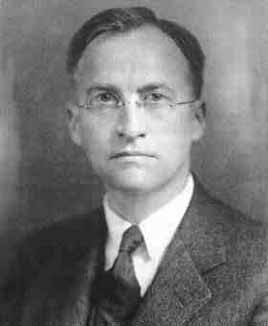
\includegraphics[height=0.42\textheight]{ch0_birkhoff_1910.jpg}\\[1mm]
\imgcap{George David Birkhoff (1884--1944)}
\imgcredit{https://commons.wikimedia.org/wiki/File:George_David_Birkhoff_1.jpg}{Photo: unknown author (c.\ 1910); public domain; Wikimedia Commons}
\end{column}
\end{columns}
\end{frame}

\begin{frame}{Mixing: dependence that fades (1/2)}
\itemsize{\small}
\begin{itemize}
    \item Strong ($\alpha$-) mixing coefficient \refRosenblatt:
    \begin{itemize}
        \item $\alpha(m) = \sup_t\,\sup\{|P(A\cap B) - P(A)P(B)|: A \in \mathcal{F}_{-\infty}^{t}, B \in \mathcal{F}_{t+m}^{\infty}\}$
        \item $\mathcal{F}_{-\infty}^{t}$: the events determined by $x_s$, $s \le t$ (the past); $\mathcal{F}_{t+m}^{\infty}$: those determined by $x_s$, $s \ge t + m$ (the future after a gap of $m$ periods)
        \item $|P(A\cap B) - P(A)P(B)|$ is 0 when $A$ and $B$ are independent: $\alpha(m)$ is the largest dependence between a past and a future event $m$ periods apart
    \end{itemize}
    \item $\alpha$-mixing: $\alpha(m) \to 0$ as $m \to \infty$, i.e.\ the distant past and future become independent
    \begin{itemize}
        \item $\beta(m) = \sup_t E\big[\sup_{B \in \mathcal{F}_{t+m}^{\infty}}|P(B \mid \mathcal{F}_{-\infty}^{t}) - P(B)|\big]$: the average gap between conditional and unconditional probabilities of future events
        \item $\varphi(m) = \sup_t\sup\{|P(B \mid A) - P(B)|: A \in \mathcal{F}_{-\infty}^{t}, P(A) > 0, B \in \mathcal{F}_{t+m}^{\infty}\}$: the worst case over past events
        \item $\alpha(m) \le \beta(m) \le \varphi(m)$: $\beta$- and $\varphi$-mixing are stronger; mixing implies ergodicity \refBradley
    \end{itemize}
\end{itemize}
\end{frame}

\begin{frame}{Mixing: dependence that fades (2/2)}
\itemsize{\small}
\begin{itemize}
    \item Models that are mixing
    \begin{itemize}
        \item stationary ARMA with continuous innovations: geometrically $\beta$-mixing \refMokkadem
        \item strictly stationary GARCH(1,1), stochastic volatility: geometrically $\beta$-mixing \refCC
        \item geometric: $\beta(m) \le C\lambda^m$ for some constants $C > 0$ and $0 < \lambda < 1$
    \end{itemize}
    \item Models that are not
    \begin{itemize}
        \item unit roots, long memory with $d > 0$ (\atschlink{https://danpele.github.io/Time-Series-Analysis/EN/Courses/chapter8_long_memory_arfima.pdf}{TSA, Chapter 8}), some deterministic chaos
        \item there mixing fails, or is too slow for the standard CLT
    \end{itemize}
    \item Mixing coefficients cannot be estimated from one path
    \begin{itemize}
        \item the assumption is checked through the model, not tested
    \end{itemize}
\end{itemize}
\end{frame}

\begin{frame}{Laws of large numbers for dependent data}
\itemsize{\small}
\begin{itemize}
    \item \textbf{$L^2$ law}: weakly stationary with $\gamma_j \to 0$ $\Rightarrow$ $E(\bar x - \mu)^2 \to 0$
    \begin{itemize}
        \item Proof: $E(\bar x - \mu)^2 = T^{-1}\sum_{|j|<T}(1 - |j|/T)\gamma_j$, and the Cesàro mean (the average of the first terms) of the sequence $\gamma_j \to 0$ tends to 0
    \end{itemize}
    \item \textbf{Ergodic law} \refBirkhoff: almost sure convergence, only $E|x_t| < \infty$, no second moment
    \begin{itemize}
        \item Covers squared returns of a GARCH with infinite fourth moment: means converge, but the CLT may fail
    \end{itemize}
    \item \textbf{Mixingales and near-epoch dependence} \refHamilton
    \begin{itemize}
        \item mixingale: $\|E(x_t - \mu \mid \mathcal{F}_{t-m})\|_2 \le c_t\,\psi_m$ with $\psi_m \to 0$: the past predicts less and less of $x_t$
        \item near-epoch dependence: $\|x_t - E(x_t \mid v_{t-m}, \dots, v_{t+m})\|_2 \to 0$ as $m \to \infty$, with $\{v_t\}$ mixing: $x_t$ is almost a function of nearby values of a mixing process
        \item $\|z\|_2 = (E z^2)^{1/2}$; $c_t$: scaling constants; these cover functions of mixing processes, e.g.\ the squares of a GARCH
    \end{itemize}
    \item Consistency (LLN) is cheap; valid standard errors (CLT plus a consistent $\hat\Omega$) are the hard part
\end{itemize}
\end{frame}

\begin{frame}{Martingale differences and their central limit theorem}
\itemsize{\small}
\begin{itemize}
    \item $\{u_t\}$ is a \textbf{martingale difference sequence} (MDS) if $E(u_t \mid \mathcal{F}_{t-1}) = 0$
    \begin{itemize}
        \item $\mathcal{F}_{t-1}$: the information available at $t-1$; the past does not predict $u_t$ on average
        \item Uncorrelated with every function of the past, but may be conditionally heteroskedastic: GARCH returns, scores of a correct likelihood, one-step forecast errors of an optimal forecast
    \end{itemize}
    \item \textbf{MDS CLT} \refBillingsley: stationary, ergodic MDS with $E u_t^2 = \sigma^2 < \infty$ $\Rightarrow$ $\sqrt{T}\,\bar u \to_d N(0, \sigma^2)$
    \begin{itemize}
        \item $\to_d$: convergence in distribution; nonstationary MDS: Lindeberg-type conditions \refBrown
        \item Here $\Omega = \gamma_0$: no autocorrelation correction is needed, only heteroskedasticity-robust errors \refWhiteH
    \end{itemize}
    \item Overlapping $h$-step forecast errors are not an MDS: they follow an MA$(h-1)$ (Section ``Overlapping observations'')
\end{itemize}
\end{frame}

\begin{frame}{Central limit theorems beyond martingale differences (1/2)}
\itemsize{\small}
\begin{itemize}
    \item \textbf{Mixing CLT} \refIbragimov: if $x_t$ is stationary and
    \begin{itemize}
        \item $E|x_t|^{2+\delta} < \infty$, $\quad \sum_m \alpha(m)^{\delta/(2+\delta)} < \infty$, $\quad \Omega > 0$ $\;\Rightarrow\;$ $\sqrt{T}(\bar x - \mu) \to_d N(0, \Omega)$
        \item $\delta > 0$: the number of moments beyond the second; $\alpha(m)$: the mixing coefficient of the previous section
        \item trade-off: more moments (larger $\delta$) allow slower mixing; the first CLT under strong mixing is \refRosenblatt
    \end{itemize}
    \item \textbf{Linear processes} \refPS: $x_t - \mu = \sum\psi_j\varepsilon_{t-j}$ with i.i.d.\ or MDS $\varepsilon_t$ and $\sum j|\psi_j| < \infty$
    \begin{itemize}
        \item the condition on $\psi_j$ requires the effect of a shock to die out fast enough
    \end{itemize}
\end{itemize}
\end{frame}

\begin{frame}{Central limit theorems beyond martingale differences (2/2)}
\itemsize{\small}
\begin{itemize}
    \item Beveridge--Nelson decomposition of the lag polynomial $\psi(L) = \sum_j\psi_jL^j$:
    \begin{itemize}
        \item $\psi(L) = \psi(1) - (1-L)\tilde\psi(L)$, $\quad$ so $\quad \sqrt{T}(\bar x - \mu) = \psi(1)\sqrt{T}\bar\varepsilon + o_p(1)$
        \item $\psi(1) = \sum_j\psi_j$: the long-run effect of a shock; $\tilde\psi(L)$: the polynomial of the transitory part; $o_p(1)$: a term that tends to 0 in probability
        \item the mean of $x_t$ behaves like $\psi(1)$ times the mean of the innovations, hence $\Omega = \sigma^2\psi(1)^2$
    \end{itemize}
    \item Functional versions (invariance principles) give the Brownian-motion limits
    \begin{itemize}
        \item they underlie the unit-root theory and the fixed-$b$ theory (next section)
    \end{itemize}
    \item All three CLTs need $0 < \Omega < \infty$
    \begin{itemize}
        \item unit roots give $\Omega = \infty$; over-differencing gives $\Omega = 0$
    \end{itemize}
\end{itemize}
\end{frame}

\begin{frame}{Information lost to dependence}
\itemsize{\footnotesize}
\begin{center}
    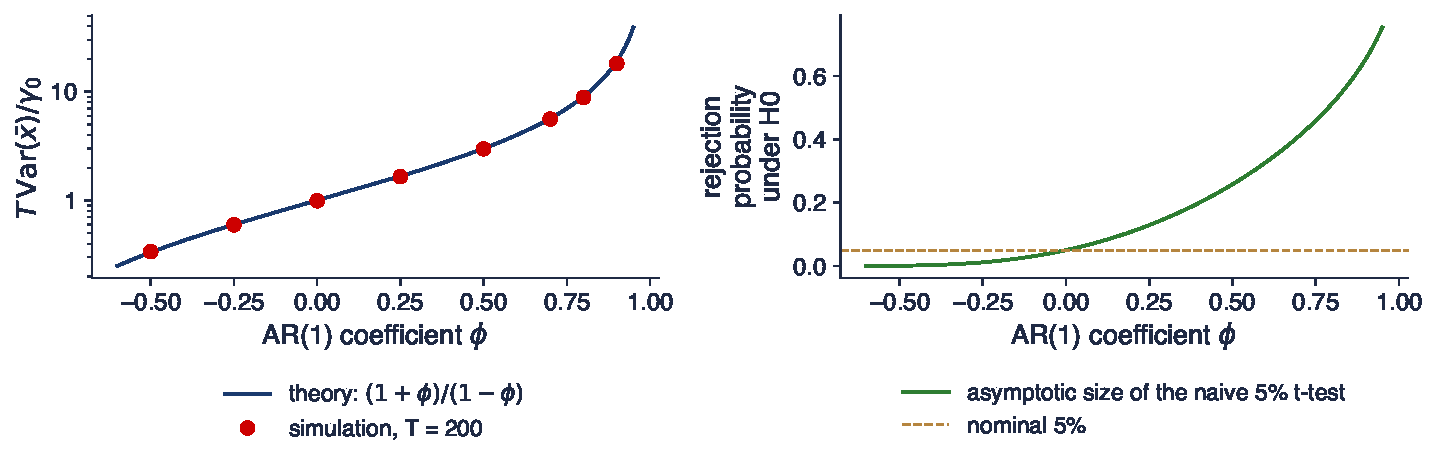
\includegraphics[width=0.97\textwidth,height=0.56\textheight,keepaspectratio]{ats_ch0_lrv_ar1.pdf}
\end{center}
\vspace{-0.25cm}
\begin{itemize}
    \item Left: $T\Var(\bar x)/\gamma_0$ for an AR(1), theory $(1+\phi)/(1-\phi)$ and 20\,000 simulations with $T = 200$; right: asymptotic size of the naive 5\% test, $2[1 - \Phi(1.96/\sqrt{(1+\phi)/(1-\phi)})]$, with $\Phi$ the standard normal distribution function
\end{itemize}
\quantlet{ATS\_ch0\_long\_run\_variance}{\qlurl{ATS_ch0_long_run_variance}}
\end{frame}

\begin{frame}{Interpreting the variance inflation}
\itemsize{\small}
\begin{itemize}
    \item $\phi = 0.5$: the factor is $3$ (simulated $2.98$); $\phi = 0.9$: $19$ (simulated $18.1$, the finite-$T$ factor $1 - |j|/T$ lowers it)
    \begin{itemize}
        \item The naive test rejects a true $H_0$ with probability $15\%$ at $\phi = 0.3$, $26\%$ at $0.5$ and $65\%$ at $0.9$
    \end{itemize}
    \item Negative dependence works the other way: $\phi = -0.5$ gives a factor $0.33$, a conservative naive test
    \begin{itemize}
        \item The S\&P 500 mean return is an example: its HAC standard error is smaller than the naive one
    \end{itemize}
    \item Confidence intervals inherit the factor: a naive 95\% interval covers $\mu$ only about $74\%$ of the time at $\phi = 0.5$
\end{itemize}
\end{frame}

\begin{frame}{Regression with dependent errors (1/2)}
\itemsize{\small}
\begin{itemize}
    \item Model $y_t = x_t'\beta + u_t$ with $E(x_t u_t) = 0$
    \begin{itemize}
        \item $x_t$: the vector of regressors; $\beta$: the coefficients; $u_t$: the error, uncorrelated with $x_t$; $'$ denotes transposition
    \end{itemize}
    \item Under a CLT for the products $x_t u_t$, the OLS estimator is asymptotically normal:
    \begin{itemize}
        \item $\sqrt{T}(\hat\beta - \beta) \to_d N\big(0,\; Q^{-1}\Omega_{xu} Q^{-1}\big)$, $\quad Q = E(x_t x_t'),\quad \Omega_{xu} = \sum_{j}E(x_t u_t u_{t-j} x_{t-j}')$
        \item $Q$: the second-moment matrix of the regressors; $\Omega_{xu}$: the long-run variance of $x_t u_t$
        \item the form $Q^{-1}\Omega_{xu}Q^{-1}$ is called a sandwich: $\Omega_{xu}$ between two copies of $Q^{-1}$
    \end{itemize}
\end{itemize}
\end{frame}

\begin{frame}{Regression with dependent errors (2/2)}
\itemsize{\small}
\begin{itemize}
    \item Scalar slope, $x_t$ and $u_t$ independent stationary series: the error factor is
    \begin{itemize}
        \item $\Omega_{xu}/(\gamma_{x,0}\gamma_{u,0}) = 1 + 2\sum_{j\ge 1}\rho_{x}(j)\rho_{u}(j)$
        \item $\gamma_{x,0}, \gamma_{u,0}$: the variances of $x_t$ and $u_t$; $\rho_x(j), \rho_u(j)$: their autocorrelations at lag $j$
    \end{itemize}
    \item A large distortion needs both a persistent regressor and a persistent error
    \begin{itemize}
        \item if either autocorrelation is zero, the factor is 1; a persistent predictor with persistent errors is the worst case
    \end{itemize}
    \item The Newey--West covariance matrix \refNW: the sandwich $\hat Q^{-1}\hat\Omega_{xu}\hat Q^{-1}$
    \begin{itemize}
        \item $\hat Q$: the sample mean of $x_tx_t'$; $\hat\Omega_{xu}$: a kernel estimate of $\Omega_{xu}$ (next section)
    \end{itemize}
\end{itemize}
\end{frame}

\begin{frame}{Recap: asymptotics for dependent data}
\itemsize{\small}
\begin{itemize}
    \item $\Var(\sqrt{T}\bar x) \to \Omega = \sum_j\gamma_j = 2\pi f(0)$; the i.i.d.\ formula keeps only $\gamma_0$
    \item Ergodicity gives the LLN; mixing or martingale structure plus moments give the CLT
    \item For an MDS, $\Omega = \gamma_0$: heteroskedasticity-robust errors suffice
    \item Positive persistence makes naive tests over-reject; negative persistence makes them conservative
\end{itemize}
\end{frame}


%=============================================================================
\section{HAC estimation}
%=============================================================================

\begin{frame}{Estimating the long-run variance}
\itemsize{\small}
\begin{itemize}
    \item Plugging in all sample autocovariances fails: $\sum_{|j|<T}\hat\gamma_j = 0$ identically for demeaned data
    \begin{itemize}
        \item high-order $\hat\gamma_j$ use few pairs and are mostly noise
    \end{itemize}
    \item \textbf{Kernel estimator}: a weighted sum of sample autocovariances
    \begin{itemize}
        \item $\hat\Omega = \sum_{|j|<T} k(j/S)\,\hat\gamma_j$, $\quad k(0) = 1$, $\quad k(x)$ decreasing in $|x|$
        \item $k(j/S)$: the weight of lag $j$; $S$: the bandwidth; equivalently a smoothed periodogram at frequency 0, $\hat\Omega = 2\pi\hat f(0)$ \refSS
    \end{itemize}
    \item Consistency: $S \to \infty$ and $S/T \to 0$, under mixing and moment conditions \refAndrews
    \begin{itemize}
        \item the down-weighted lags create bias, the included ones create variance: $S$ balances the two
    \end{itemize}
    \item A variance estimator must be nonnegative: not every kernel guarantees this
\end{itemize}
\end{frame}

\begin{frame}{Case study: Newey and West (1987) (1/2)}
\itemsize{\small}
\begin{itemize}
    \item \refNW, Econometrica 55(3): the Bartlett kernel $k(x) = 1 - |x|$ for $|x| \le 1$, with $L$ lags
    \begin{itemize}
        \item $\hat\Omega_{NW} = \hat\Gamma_0 + \sum_{j=1}^{L}\Big(1 - \dfrac{j}{L+1}\Big)\big(\hat\Gamma_j + \hat\Gamma_j'\big)$, $\quad\hat\Gamma_j = T^{-1}\sum_{t>j}\hat h_t\hat h_{t-j}'$
    \end{itemize}
    \item Notation
    \begin{itemize}
        \item $\hat h_t = x_t\hat u_t$: regressor times OLS residual $\hat u_t$ (the score of observation $t$)
        \item $\hat\Gamma_j$: the sample autocovariance matrix of $\hat h_t$ at lag $j$; $\hat\Gamma_0$: its variance matrix
        \item $1 - j/(L+1)$: weights that decrease linearly from 1 to $1/(L+1)$; lags beyond $L$ get weight 0
    \end{itemize}
\end{itemize}
\end{frame}

\begin{frame}{Case study: Newey and West (1987) (2/2)}
\itemsize{\small}
\begin{itemize}
    \item \textbf{Positive semi-definite by construction}: Bartlett weights are the autocovariances of a moving sum
    \begin{itemize}
        \item up to end effects, $\hat\Omega_{NW} = \frac{1}{(L+1)T}\sum_t\big(\sum_{i=0}^{L}\hat h_{t-i}\big)\big(\sum_{i=0}^{L}\hat h_{t-i}\big)'$
        \item a sum of outer products $vv'$, each positive semi-definite, so the sum is too
        \item spectral view: the Bartlett (Fejér) window is nonnegative at every frequency
    \end{itemize}
    \item Consistency with $L \to \infty$, $L = o(T^{1/4})$ in the original paper
    \begin{itemize}
        \item $L = o(T^{1/4})$: $L$ grows more slowly than $T^{1/4}$; \refAndrews{} refines the rates
    \end{itemize}
    \item One page of algebra, now the default robust standard error in every econometrics package
\end{itemize}
\end{frame}

\begin{frame}{A truncated kernel can give a negative variance}
\itemsize{\small}
\begin{itemize}
    \item Truncated (uniform) kernel: $k(x) = 1$ for $|x| \le 1$: $\hat\Omega = \hat\gamma_0 + 2\sum_{j=1}^{L}\hat\gamma_j$ (used by \refHH{} for overlapping forecasts)
    \begin{itemize}
        \item Exactly right when $\gamma_j = 0$ for $j > L$, e.g.\ an MA$(h-1)$ forecast error with $L = h - 1$
    \end{itemize}
    \item Ten observations alternating in sign, $(1, -1, 1, -1, 1, -1, 1, -1, 2, -2)$: $\hat\gamma_0 = 1.6$, $\hat\gamma_1 = \ensuremath{-}1.3$, $\hat\gamma_2 = 1.0$
    \begin{itemize}
        \item Truncated, $L = 1$: $\hat\gamma_0 + 2\hat\gamma_1 = \ensuremath{-}1.0 < 0$
        \item Bartlett, $L = 1$: $\hat\gamma_0 + \hat\gamma_1 = 0.3 > 0$
    \end{itemize}
    \item Lesson: a negative variance is not a numerical accident; it is a property of the kernel (Seminar 0, A3--A4)
\end{itemize}
\end{frame}

\begin{frame}{Kernels}
\itemsize{\footnotesize}
\begin{center}
    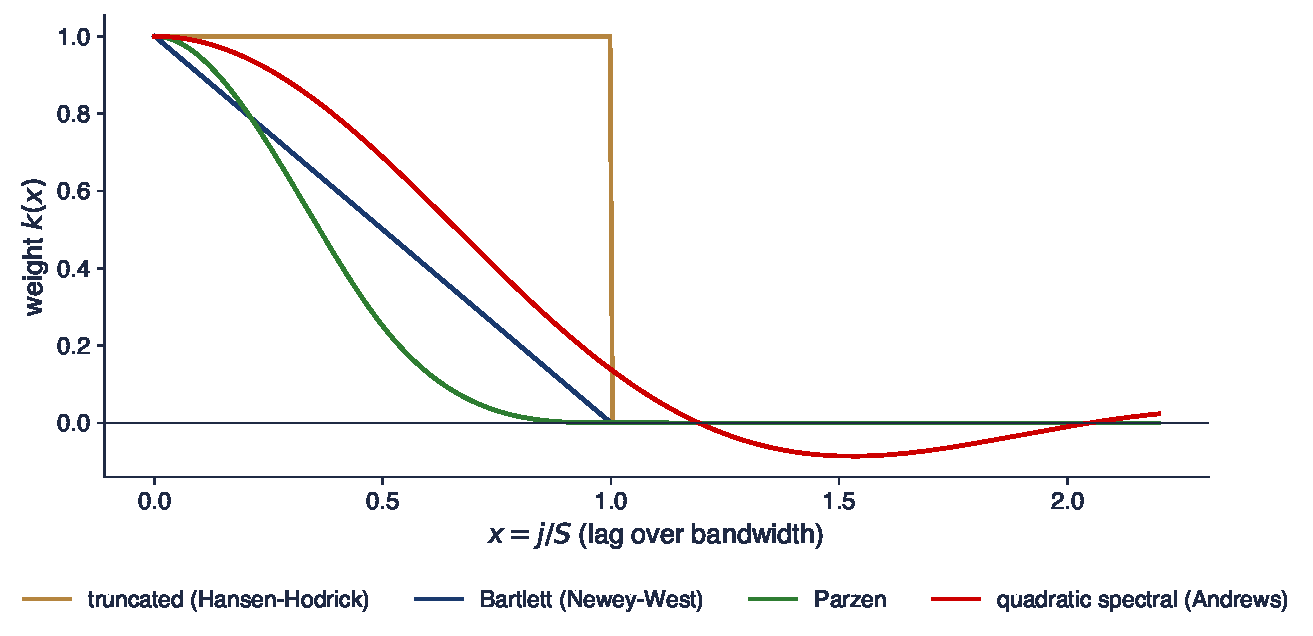
\includegraphics[width=0.97\textwidth,height=0.52\textheight,keepaspectratio]{ats_ch0_kernels.pdf}
\end{center}
\vspace{-0.25cm}
\begin{itemize}
    \item Weight $k(x)$ against $x = j/S$, the lag relative to the bandwidth; Bartlett: $1 - |x|$ ($|x| \le 1$)
    \item Parzen: $1 - 6x^2 + 6|x|^3$ ($|x| \le 1/2$), $2(1-|x|)^3$ ($1/2 < |x| \le 1$); QS (quadratic spectral): $\frac{25}{12\pi^2x^2}\big[\frac{\sin(6\pi x/5)}{6\pi x/5} - \cos(6\pi x/5)\big]$, all lags
\end{itemize}
\quantlet{ATS\_ch0\_long\_run\_variance}{\qlurl{ATS_ch0_long_run_variance}}
\end{frame}

\begin{frame}{Interpreting the kernels}
\itemsize{\small}
\begin{itemize}
    \item Bartlett, Parzen and QS have nonnegative spectral windows (the Fourier transform of the weights): $\hat\Omega \ge 0$ always
    \begin{itemize}
        \item QS takes small negative weights (minimum $\ensuremath{-}0.086$) yet stays positive semi-definite
    \end{itemize}
    \item Kernel order $q$: $1 - k(x) \sim c|x|^q$ near 0, with $c > 0$ a constant; Bartlett $q = 1$, Parzen and QS $q = 2$
    \begin{itemize}
        \item bias of order $S^{-q}$, variance of order $S/T$: the optimal $S$ grows like $T^{1/(2q+1)}$
        \item i.e.\ $T^{1/3}$ for Bartlett and $T^{1/5}$ for QS
    \end{itemize}
    \item \refAndrews: QS minimises the asymptotic MSE among kernels with nonnegative estimates
\end{itemize}
\end{frame}

\begin{frame}{Case study: Andrews (1991) and the choice of bandwidth (1/2)}
\itemsize{\small}
\begin{itemize}
    \item MSE-optimal bandwidth \refAndrews: the $S$ that minimises the mean squared error of $\hat\Omega$
    \begin{itemize}
        \item $S^* = c_k\,(\alpha(q)\,T)^{1/(2q+1)}$
        \item $q$: the order of the kernel; $c_k$: a constant of the kernel; $\alpha(q)$: a function of the unknown spectrum, large for persistent series
        \item Bartlett: $S^* = 1.1447(\hat\alpha(1)T)^{1/3}$; Parzen: $2.6614(\hat\alpha(2)T)^{1/5}$; QS: $1.3221(\hat\alpha(2)T)^{1/5}$
    \end{itemize}
    \item \textbf{AR(1) plug-in}: fit an AR(1) with coefficient $\hat\rho$ to $\hat h_t$, then
    \begin{itemize}
        \item $\hat\alpha(1) = \dfrac{4\hat\rho^2}{(1-\hat\rho)^2(1+\hat\rho)^2}$, $\qquad \hat\alpha(2) = \dfrac{4\hat\rho^2}{(1-\hat\rho)^4}$
        \item both grow without bound as $\hat\rho \to 1$: more persistence, wider bandwidth
    \end{itemize}
\end{itemize}
\end{frame}

\begin{frame}{Case study: Andrews (1991) and the choice of bandwidth (2/2)}
\itemsize{\small}
\begin{itemize}
    \item Newey--West rule of thumb: $L = \lfloor 4(T/100)^{2/9}\rfloor$
    \begin{itemize}
        \item $\lfloor\cdot\rfloor$: the integer part; $L$ depends only on $T$, not on the data
        \item their nonparametric automatic selection \refNWb{} estimates the spectrum instead
    \end{itemize}
    \item Prewhitening with a VAR(1), then recolouring \refAM
    \begin{itemize}
        \item filter out the AR(1) part, estimate $\Omega$ on the residuals, then undo the filter: less bias for persistent series
    \end{itemize}
    \item The MSE criterion targets $\hat\Omega$, not the test
    \begin{itemize}
        \item this is the source of the size distortions of the next sections
    \end{itemize}
\end{itemize}
\end{frame}

\begin{frame}{HAC standard errors as a function of the bandwidth}
\itemsize{\footnotesize}
\begin{center}
    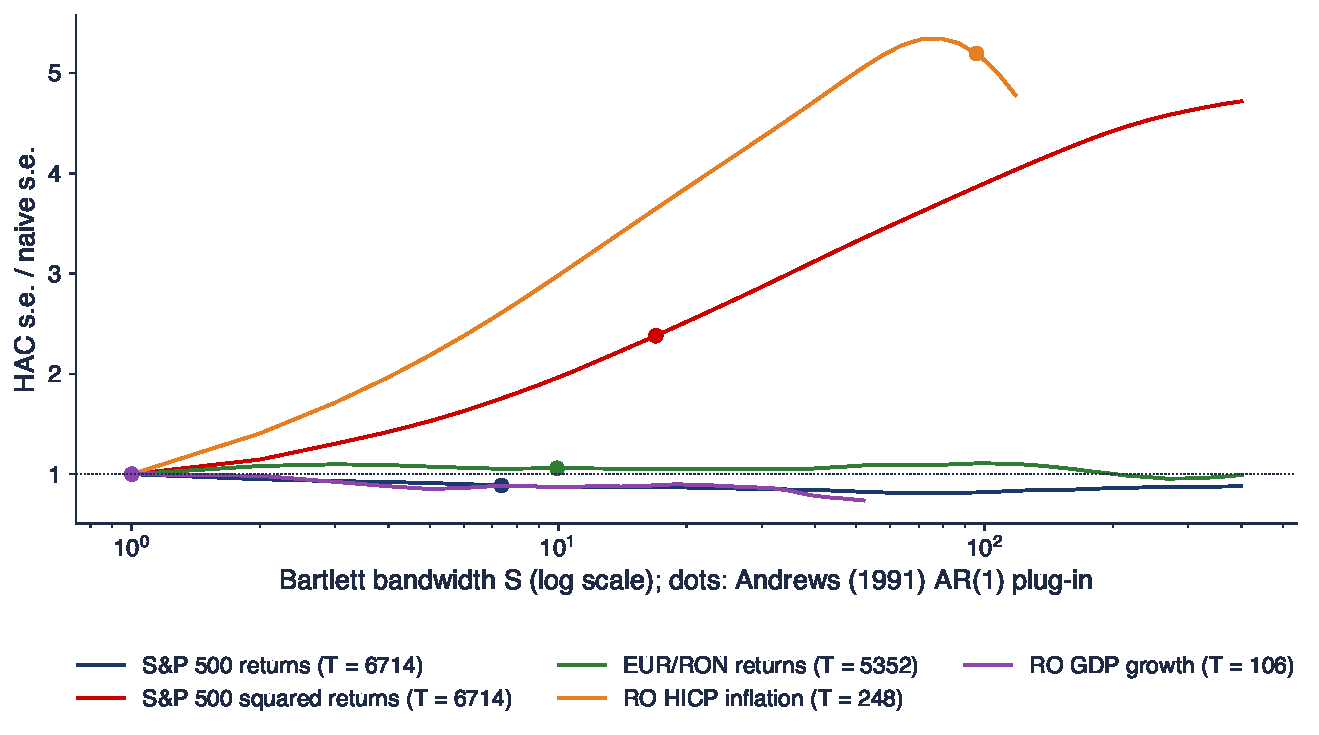
\includegraphics[width=0.97\textwidth,height=0.56\textheight,keepaspectratio]{ats_ch0_hac_bandwidth.pdf}
\end{center}
\vspace{-0.25cm}
\begin{itemize}
    \item Ratio of the Bartlett HAC standard error of the mean to the naive one, $S$ from 1 to $\min(400, T/2)$; dots: Andrews AR(1) plug-in
\end{itemize}
\quantlet{ATS\_ch0\_hac}{\qlurl{ATS_ch0_hac}}
\end{frame}

\begin{frame}{Interpreting the bandwidth paths}
\itemsize{\small}
\begin{itemize}
    \item Squared S\&P 500 returns: ratio $2.04$ with the rule of thumb ($S = 11$), $2.38$ with Andrews ($S = 17$), still rising to $4.72$ at $S = 400$
    \begin{itemize}
        \item No plateau: the AR(1) plug-in misses the slow decay of volatility autocorrelation (long memory, \atschlink{https://danpele.github.io/Advanced-Time-Series/EN/Courses/chapter10_long_memory_rough_volatility.pdf}{Chapter 10})
    \end{itemize}
    \item Romanian inflation: $2.18$ with the rule of thumb, $5.19$ with Andrews ($S = 96$ months)
    \begin{itemize}
        \item The rule of thumb ignores the data: with $T$ fixed it gives the same $S$ for white noise and for a near unit root
    \end{itemize}
    \item S\&P 500 returns: ratio below 1 at every $S$ (negative $\hat\rho_1$); EUR/RON: flat near $1.06$
\end{itemize}
\end{frame}

\begin{frame}{Fixed-$b$ asymptotics}
\itemsize{\small}
\begin{itemize}
    \item Standard theory: $S/T \to 0$, $\hat\Omega \to_p \Omega$, the $t$-statistic is $N(0,1)$
    \begin{itemize}
        \item $\to_p$: convergence in probability; the sampling error of $\hat\Omega$ is ignored
        \item with 100--300 observations, $\hat\Omega$ is noisy and biased downwards: the normal critical values are too small
    \end{itemize}
    \item \textbf{Fixed-$b$} \refKVB, \refKVb, \refKV: keep $b = S/T$ fixed as $T \to \infty$
    \begin{itemize}
        \item $\hat\Omega/\Omega \to_d Q_k(b)$, $\qquad t \to_d W(1)/\sqrt{Q_k(b)}$
        \item $W(r)$: a standard Brownian motion on $r \in [0,1]$ ($r$: the fraction of the sample); $Q_k(b)$: a random functional of the Brownian bridge $\tilde W(r) = W(r) - rW(1)$
        \item Bartlett kernel: $Q(b) = \frac{2}{b}\int_0^1 \tilde W(r)^2\,dr - \frac{2}{b}\int_0^{1-b}\tilde W(r+b)\tilde W(r)\,dr$ \refKV
        \item nonstandard but pivotal (free of unknown parameters): critical values depend only on the kernel and on $b$
    \end{itemize}
    \item Higher-order theory: fixed-$b$ critical values remove the leading size distortion of the normal approximation \refSPJ
\end{itemize}
\end{frame}

\begin{frame}{Fixed-$b$ critical values}
\itemsize{\footnotesize}
\begin{center}
    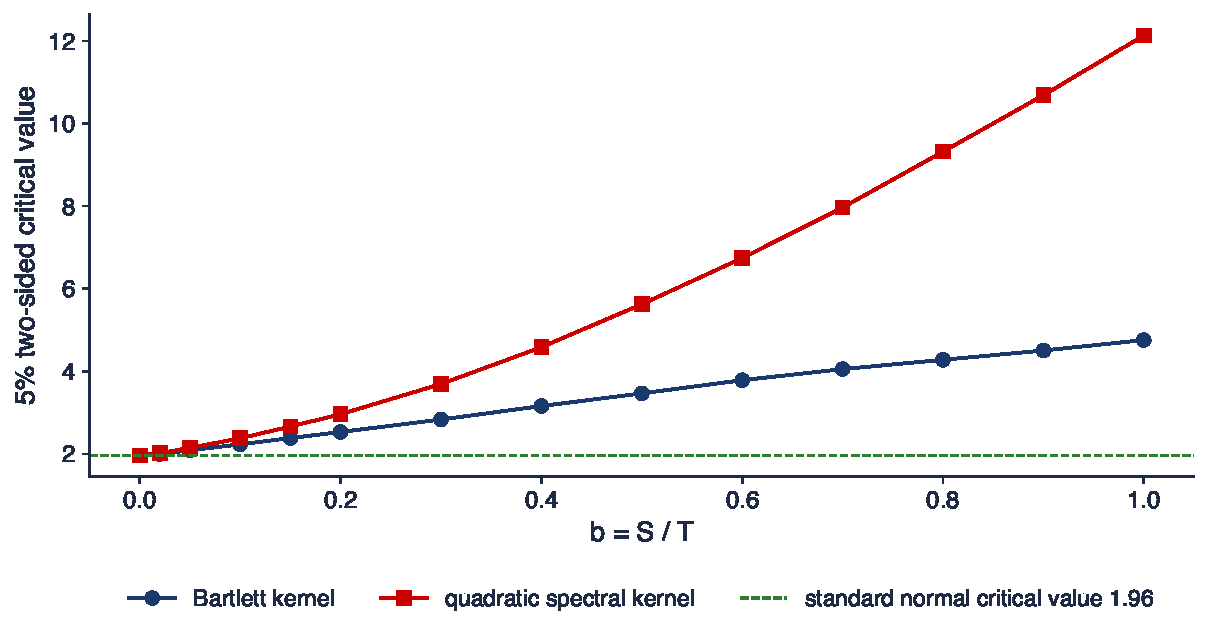
\includegraphics[width=0.97\textwidth,height=0.55\textheight,keepaspectratio]{ats_ch0_fixed_b.pdf}
\end{center}
\vspace{-0.25cm}
\begin{itemize}
    \item Two-sided 5\% critical values of the $t$-test for a mean with $S = bT$, simulated (20\,000 i.i.d.\ normal samples, $T = 500$)
\end{itemize}
\quantlet{ATS\_ch0\_hac}{\qlurl{ATS_ch0_hac}}
\end{frame}

\begin{frame}{Interpreting the fixed-$b$ critical values}
\itemsize{\small}
\begin{itemize}
    \item Bartlett: $2.23$ at $b = 0.1$, $3.47$ at $b = 0.5$, $4.76$ at $b = 1$ (Kiefer--Vogelsang--Bunzel statistic)
    \begin{itemize}
        \item Close to the cubic approximation reported in \refKV{} for the Bartlett kernel
    \end{itemize}
    \item QS: $2.38$ at $b = 0.1$ and $5.62$ at $b = 0.5$: QS with a large $b$ is very noisy
    \item Larger $b$: less bias in $\hat\Omega$, more variance, compensated by a larger critical value: better size, lower power
    \item What do you think? Why does the critical value at $b \to 0$ tend to 1.96?
    \begin{itemize}
        \item Answer: as $b \to 0$, $Q_k(b) \to 1$ ($\hat\Omega$ becomes consistent), so $t \to_d W(1) \sim N(0,1)$: the standard asymptotics return
    \end{itemize}
\end{itemize}
\end{frame}

\begin{frame}{Recommendations for practice: Lazarus, Lewis, Stock and Watson (2018) (1/2)}
\itemsize{\small}
\begin{itemize}
    \item \refLLSW{} choose the bandwidth for the \emph{test}: a size--power frontier, not the MSE of $\hat\Omega$
    \begin{itemize}
        \item first recommendation: Newey--West with $S = 1.3\sqrt{T}$ and fixed-$b$ critical values
    \end{itemize}
    \item Second recommendation: the equal-weighted cosine (EWC) estimator
    \begin{itemize}
        \item $\hat\Omega = \nu^{-1}\sum_{j=1}^{\nu}\hat\Lambda_j^2$, $\qquad \hat\Lambda_j = \sqrt{2/T}\sum_t \cos[\pi j(t - 1/2)/T]\,\hat h_t$, $\qquad \nu = 0.4T^{2/3}$
        \item $\hat\Lambda_j$: the projection of $\hat h_t$ on the $j$-th cosine, a low-frequency component; each $\hat\Lambda_j^2$ estimates $\Omega$
        \item $\nu$: the number of cosines averaged, also the degrees of freedom: critical values from Student $t_\nu$
    \end{itemize}
\end{itemize}
\end{frame}

\begin{frame}{Recommendations for practice: Lazarus, Lewis, Stock and Watson (2018) (2/2)}
\itemsize{\small}
\begin{itemize}
    \item The size--power trade-off is unavoidable
    \begin{itemize}
        \item \refLLS{} give the frontier for kernel tests
    \end{itemize}
    \item Very persistent series ($\phi$ near 1): no kernel or EWC rule is reliable
    \begin{itemize}
        \item \refMuller{} proposes tests valid under local-to-unity dependence (a root that tends to 1 as $T$ grows)
    \end{itemize}
    \item These are the defaults of the course from \atschlink{https://danpele.github.io/Advanced-Time-Series/EN/Courses/chapter1_forecast_evaluation.pdf}{Chapter 1} on
\end{itemize}
\end{frame}

\begin{frame}{Recap: HAC estimation}
\itemsize{\small}
\begin{itemize}
    \item Kernel estimators down-weight distant lags; Bartlett (Newey--West), Parzen and QS are always nonnegative; the truncated kernel is not
    \item The \refAndrews{} bandwidths are MSE-optimal for $\hat\Omega$ and adapt to persistence; the rule of thumb does not
    \item Fixed-$b$ critical values account for the noise in $\hat\Omega$; LLSW: NW with $S = 1.3\sqrt{T}$ or EWC with $\nu = 0.4T^{2/3}$
\end{itemize}
\end{frame}


%=============================================================================
\section{Size distortions: a Monte Carlo study}
%=============================================================================

\begin{frame}{Monte Carlo design}
\itemsize{\small}
\begin{itemize}
    \item DGP: $x_t = \phi x_{t-1} + \varepsilon_t$, $\varepsilon_t \sim N(0,1)$ i.i.d., 200 burn-in values; $H_0: \mu = 0$ is true
    \begin{itemize}
        \item $\phi$: the AR(1) coefficient, i.e.\ the persistence; burn-in: initial values dropped so that the series starts from its stationary distribution
        \item $\phi \in \{0, 0.3, 0.5, 0.7, 0.9\}$, $T \in \{100, 400\}$; 5\,000 replications (1\,000 for the bootstrap, 399 resamples each); seed 2026
    \end{itemize}
    \item Seven tests at nominal 5\%
    \begin{itemize}
        \item naive i.i.d.; NW rule of thumb; NW and QS with the Andrews AR(1) bandwidth (normal critical values)
        \item NW with $S = 1.3\sqrt{T}$ and fixed-$b$ values; EWC with $t_\nu$; circular block bootstrap with the Politis--White block length
    \end{itemize}
    \item Monte Carlo standard error of a rejection rate $p$ estimated from $R$ replications: $\sqrt{p(1-p)/R}$
    \begin{itemize}
        \item about $0.3$ percentage points (pp) at $p = 5\%$ and $R = 5000$
    \end{itemize}
    \item The same design as the Monte Carlo sections of \refAndrews{} and \refKV: AR(1) data, rejection rates under the null
\end{itemize}
\end{frame}

\begin{frame}{Size of seven tests under AR(1) dependence}
\itemsize{\footnotesize}
\begin{center}
    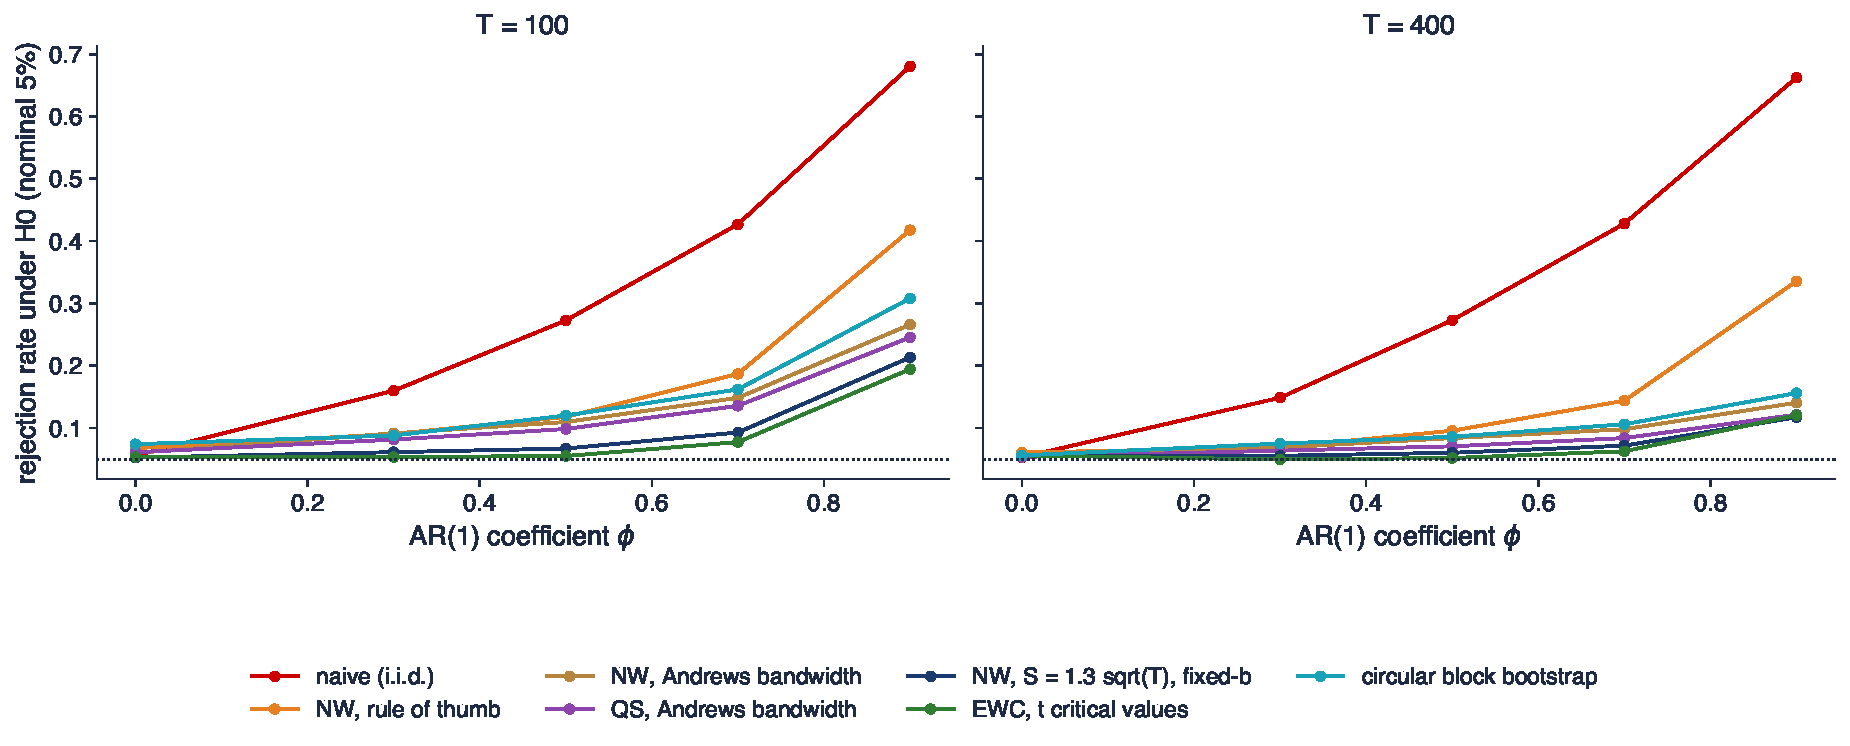
\includegraphics[width=0.97\textwidth,height=0.58\textheight,keepaspectratio]{ats_ch0_mc_size.pdf}
\end{center}
\vspace{-0.25cm}
\begin{itemize}
    \item Rejection rate of $H_0: \mu = 0$ (true) against $\phi$; dotted line: 5\%
\end{itemize}
\quantlet{ATS\_ch0\_size\_monte\_carlo}{\qlurl{ATS_ch0_size_monte_carlo}}
\end{frame}

\begin{frame}{Size in numbers (\%)}
\itemsize{\footnotesize}
\begin{center}
\footnotesize
\begin{tabular}{lrrrrrr}
\toprule
& \multicolumn{3}{c}{$T = 100$} & \multicolumn{3}{c}{$T = 400$} \\
Test & $\phi = 0$ & $0.5$ & $0.9$ & $\phi = 0$ & $0.5$ & $0.9$ \\
\midrule
naive i.i.d. & 5.6 & 27.3 & 68.1 & 5.3 & 27.3 & 66.2 \\
NW, rule of thumb & 6.8 & 11.8 & 41.8 & 6.1 & 9.6 & 33.6 \\
NW, Andrews & 6.0 & 11.0 & 26.6 & 5.3 & 8.4 & 14.1 \\
QS, Andrews & 6.1 & 9.8 & 24.6 & 5.4 & 7.1 & 12.1 \\
NW, $1.3\sqrt{T}$, fixed-$b$ & 5.2 & 6.7 & 21.3 & 5.6 & 6.0 & 11.7 \\
EWC, $t_\nu$ & 5.3 & 5.5 & 19.4 & 5.6 & 5.2 & 12.1 \\
circular block bootstrap & 7.4 & 12.0 & 30.8 & 5.6 & 8.6 & 15.6 \\
\bottomrule
\end{tabular}
\end{center}
\begin{itemize}
    \item Monte Carlo standard errors: about 0.3 pp near 5\%, about 0.7 pp near 30\% (bootstrap rows: about twice as large)
\end{itemize}
\end{frame}

\begin{frame}{Interpreting the Monte Carlo}
\itemsize{\footnotesize}
\begin{itemize}
    \item Naive test: $27.3\%$ at $\phi = 0.5$ and $68.1\%$ at $\phi = 0.9$; more data do not help ($66.2\%$ at $T = 400$)
    \begin{itemize}
        \item The distortion is a property of the estimator, not of the sample size
    \end{itemize}
    \item NW with the rule of thumb: $41.8\%$ at $\phi = 0.9$, $T = 100$; Andrews bandwidths halve the excess; fixed-$b$ and EWC come closest ($21.3\%$, $19.4\%$)
    \begin{itemize}
        \item At $T = 400$ and $\phi = 0.5$: $6.0\%$ and $5.2\%$, essentially exact
    \end{itemize}
    \item The block bootstrap is not a free lunch: $30.8\%$ at $\phi = 0.9$, $T = 100$, between NW and fixed-$b$
    \item Our inflation series has $\hat\rho_1 = 0.98$: outside the range where any of these tests is reliable (AI mini-case)
\end{itemize}
\end{frame}

\begin{frame}{Recap: size distortions}
\itemsize{\small}
\begin{itemize}
    \item Always report the actual size of the procedure you use, at the persistence of your data
    \item Fixed-$b$ NW and EWC (\refLLSW) dominate the classical choices in size at a modest cost in power
    \item A Monte Carlo is an experiment: fix the seed, report $R$ and the Monte Carlo standard error
\end{itemize}
\end{frame}


%=============================================================================
\section{Bootstrap for dependent data}
%=============================================================================

\begin{frame}{The failure of the i.i.d.\ bootstrap}
\itemsize{\footnotesize}
\begin{columns}[T]
\begin{column}{0.66\textwidth}
\begin{itemize}
    \item Efron's bootstrap \refEfron{} resamples single observations: the dependence is destroyed
    \begin{itemize}
        \item a star marks a bootstrap quantity: $\bar x^*$ is the mean of one resample, $\Var^*$ the variance over resamples
        \item $\Var^*(\sqrt{T}\bar x^*) = \hat\gamma_0$, not $\Omega$: the i.i.d.\ bootstrap reproduces the naive standard error
    \end{itemize}
    \item \refSingh: even for $m$-dependent data (independent beyond distance $m$) the i.i.d.\ bootstrap of the mean is inconsistent
    \begin{itemize}
        \item Idea of the block bootstrap: resample blocks long enough to keep the dependence inside them
    \end{itemize}
    \item Price to pay: dependence across block joints is lost, and the block length becomes a tuning parameter
\end{itemize}
\end{column}
\begin{column}{0.30\textwidth}
\centering
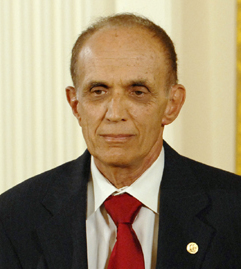
\includegraphics[height=0.40\textheight]{ch0_efron_2007.jpg}\\[1mm]
\imgcap{Bradley Efron (2007)}
\imgcredit{https://commons.wikimedia.org/wiki/File:Bradley_Efron_National_Medal_of_Science_2007_(cropped).jpg}{Photo: Ryan K. Morris, NSTMF (2007); public domain; Wikimedia Commons}
\end{column}
\end{columns}
\end{frame}

\begin{frame}{Case study: the moving-block bootstrap of Künsch (1989)}
\itemsize{\footnotesize}
\begin{columns}[T]
\begin{column}{0.64\textwidth}
\begin{itemize}
    \item \refKunsch: overlapping blocks $B_i = (x_i, \dots, x_{i+l-1})$ of length $l$, $i = 1, \dots, T - l + 1$
    \begin{itemize}
        \item draw $k = \lceil T/l\rceil$ blocks with replacement ($\lceil\cdot\rceil$: rounding up), concatenate, keep the first $T$ values
    \end{itemize}
    \item Consistency for smooth functions of means if $l \to \infty$, $l/T \to 0$
    \begin{itemize}
        \item $\Var^*(\sqrt{T}\bar x^*) \approx \sum_{|j|<l}(1 - |j|/l)\hat\gamma_j$: a Bartlett estimate with $S = l$
        \item Optimal $l \propto T^{1/3}$ for variance and bias, as for the Bartlett bandwidth \refLahiri
    \end{itemize}
    \item Edge effect: end observations enter fewer blocks, so $E^*\bar x^* \ne \bar x$
    \begin{itemize}
        \item $E^*$: the expectation over resamples; centre the bootstrap statistics at $E^*\bar x^*$
    \end{itemize}
\end{itemize}
\end{column}
\begin{column}{0.32\textwidth}
\centering
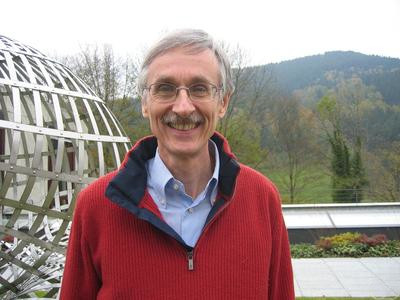
\includegraphics[height=0.34\textheight]{ch0_kunsch_2007.jpg}\\[1mm]
\imgcap{Hans Rudolf Künsch (2007)}
\imgcredit{https://commons.wikimedia.org/wiki/File:Hans-Rudolf_Künsch.jpg}{Photo: Renate Schmid (2007); CC BY-SA 2.0 de; Wikimedia Commons}
\end{column}
\end{columns}
\end{frame}

\begin{frame}{Circular and stationary bootstrap}
\itemsize{\footnotesize}
\begin{itemize}
    \item \textbf{Circular block bootstrap} (\refPRc; \refLahiri): wrap the data on a circle, $x_{T+i} = x_i$
    \begin{itemize}
        \item Every observation enters $l$ blocks: $E^*\bar x^* = \bar x$ exactly (Seminar 0, A5--A6)
    \end{itemize}
    \item \textbf{Stationary bootstrap} \refPR: block lengths geometric with mean $1/p$, uniform starting points, data wrapped on a circle
    \begin{itemize}
        \item Equivalently: each step continues the block with probability $1 - p$ or jumps to a random point with probability $p$
        \item The resampled series is stationary; the method is less sensitive to the choice of $1/p$ than MBB to $l$
    \end{itemize}
    \item Efficiency: MBB and CBB have a smaller asymptotic MSE for the variance than the stationary bootstrap at their optimal lengths \refLahiri
    \item The stationary bootstrap is the engine of the Reality Check \refWhite{} and of the SPA test (\atschlink{https://danpele.github.io/Advanced-Time-Series/EN/Courses/chapter1_forecast_evaluation.pdf}{Chapter 1})
\end{itemize}
\end{frame}

\begin{frame}{Choosing the block length (1/2)}
\itemsize{\small}
\begin{itemize}
    \item \refPW, corrected by \refPPW: plug-in estimate of the MSE-optimal mean block length
    \begin{itemize}
        \item $\hat b_{opt} = \Big(\dfrac{2\hat G^2}{\hat D}\Big)^{1/3} T^{1/3}$, $\quad \hat G = \sum_{|k|\le M}\lambda(k/M)\,|k|\,\hat\gamma_k$, $\quad \hat g = \sum_{|k|\le M}\lambda(k/M)\,\hat\gamma_k$
        \item $\hat D_{SB} = 2\hat g^2$ (stationary), $\hat D_{CB} = \tfrac{4}{3}\hat g^2$ (circular)
    \end{itemize}
    \item Notation
    \begin{itemize}
        \item $\hat G$: autocovariances weighted by their lag, the bias term; $\hat g$: an estimate of $\Omega$; $\hat D$: the variance term
        \item $\lambda$: the flat-top (trapezoid) kernel; $M = 2\hat m$: the truncation lag
        \item $\hat m$: the first lag after which $K_T$ consecutive autocorrelations are insignificant
    \end{itemize}
\end{itemize}
\end{frame}

\begin{frame}{Choosing the block length (2/2)}
\itemsize{\small}
\begin{itemize}
    \item The same structure as the Andrews bandwidth
    \begin{itemize}
        \item bias term $G$ over variance term $D$, rate $T^{1/3}$: persistent series get longer blocks
    \end{itemize}
    \item Implemented in the Python package \texttt{arch} (\texttt{optimal\_block\_length})
    \item Our data
    \begin{itemize}
        \item about 145 days for squared S\&P 500 returns, 25 months for inflation
        \item 0.8 for GDP growth, i.e.\ the i.i.d.\ bootstrap
    \end{itemize}
\end{itemize}
\end{frame}

\begin{frame}{The wild bootstrap and its limits (1/2)}
\itemsize{\small}
\begin{itemize}
    \item \textbf{Wild bootstrap} \refWu, \refLiu, \refMammen: each residual is multiplied by a random sign-like weight
    \begin{itemize}
        \item $y_t^* = x_t'\hat\beta + \hat u_t\eta_t$, $\quad \eta_t$ i.i.d., $E\eta_t = 0$, $E\eta_t^2 = 1$
        \item $y_t^*$: the bootstrap observation; $\eta_t$: Rademacher ($\pm 1$ with probability $1/2$ each) or the Mammen two-point distribution
    \end{itemize}
    \item It keeps the heteroskedasticity of each $\hat u_t$ and destroys every autocorrelation
    \begin{itemize}
        \item valid when the scores are an MDS: AR models with GARCH-type errors \refGK
        \item \textbf{not} valid for overlapping forecasts, local projections or the mean of squared returns
    \end{itemize}
\end{itemize}
\end{frame}

\begin{frame}{The wild bootstrap and its limits (2/2)}
\itemsize{\small}
\begin{itemize}
    \item Dependent wild bootstrap \refShao: $\eta_t$ drawn from a stationary process
    \begin{itemize}
        \item $\Corr(\eta_t, \eta_s) = a(|t-s|/l)$, with $a(\cdot)$ a kernel and $l$ a bandwidth
        \item wild in form, block-like in effect: neighbouring residuals keep their joint signs
    \end{itemize}
    \item Sieve bootstrap \refBuhlmann: fit an AR$(p)$ with $p \to \infty$, resample its residuals
    \begin{itemize}
        \item efficient for linear processes, fragile for nonlinear ones
    \end{itemize}
\end{itemize}
\end{frame}

\begin{frame}{Three bootstraps of one mean}
\itemsize{\footnotesize}
\begin{center}
    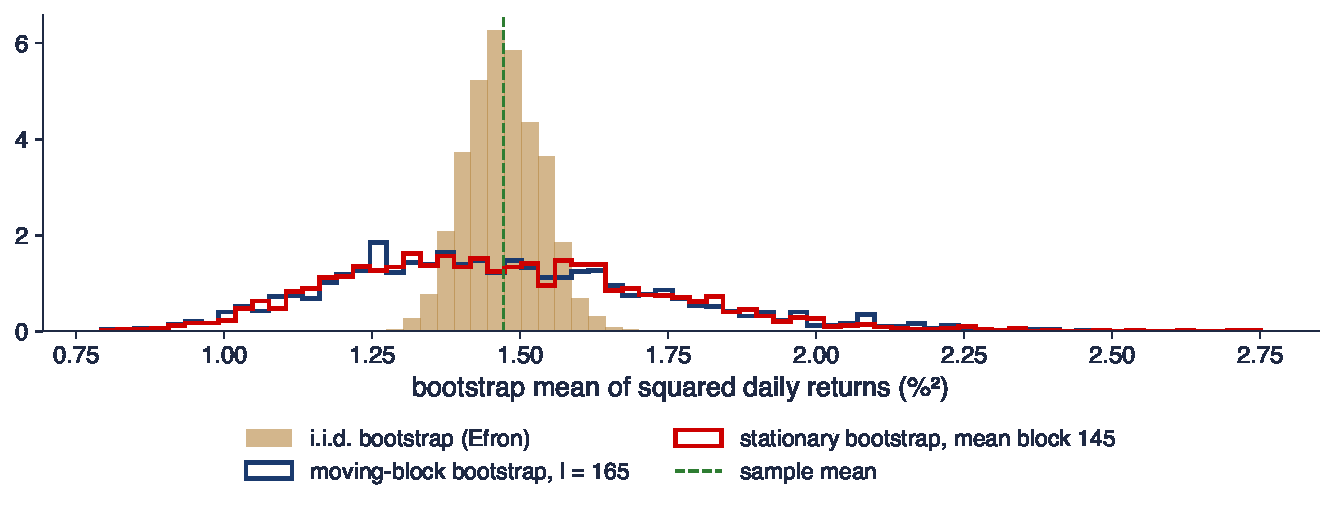
\includegraphics[width=0.97\textwidth,height=0.56\textheight,keepaspectratio]{ats_ch0_bootstrap.pdf}
\end{center}
\vspace{-0.25cm}
\begin{itemize}
    \item Mean of squared daily S\&P 500 returns ($1.472$, $T = 6\,714$); 1999 resamples each; block lengths from Politis--White
\end{itemize}
\quantlet{ATS\_ch0\_block\_bootstrap}{\qlurl{ATS_ch0_block_bootstrap}}
\end{frame}

\begin{frame}{Interpreting the three bootstraps}
\itemsize{\small}
\begin{itemize}
    \item i.i.d.\ bootstrap: standard error $0.063$, equal to the naive $0.064$, as theory says
    \begin{itemize}
        \item Block bootstraps: MBB $0.276$, CBB $0.268$, stationary $0.269$: about 4.2 times the naive value
    \end{itemize}
    \item HAC with the Andrews bandwidth: $0.152$ (about 2.4 times the naive value): smaller than the block bootstraps
    \begin{itemize}
        \item Block length 145 against an Andrews bandwidth of 17: two plug-in rules, two different views of the same slowly decaying ACF
    \end{itemize}
    \item When two valid methods disagree by a factor of two, report both and explain why: here, the volatility of volatility has long memory
\end{itemize}
\end{frame}

\begin{frame}{Bootstrap standard error against the block length}
\itemsize{\footnotesize}
\begin{center}
    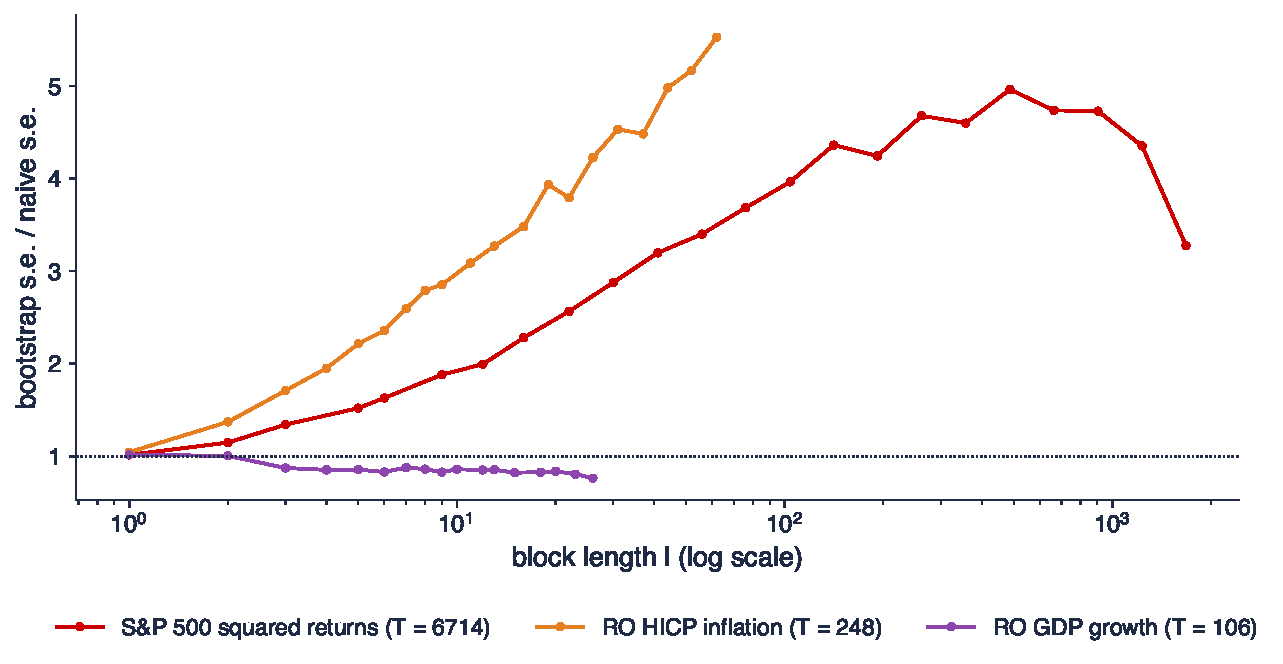
\includegraphics[width=0.97\textwidth,height=0.55\textheight,keepaspectratio]{ats_ch0_block_length.pdf}
\end{center}
\vspace{-0.25cm}
\begin{itemize}
    \item Circular block bootstrap, 999 resamples per length; ratio to the naive standard error
\end{itemize}
\quantlet{ATS\_ch0\_block\_bootstrap}{\qlurl{ATS_ch0_block_bootstrap}}
\end{frame}

\begin{frame}{Interpreting the block-length paths}
\itemsize{\small}
\begin{itemize}
    \item $l = 1$ is the i.i.d.\ bootstrap (ratio 1); the ratio grows with $l$ while $l$ is shorter than the memory of the series
    \begin{itemize}
        \item Inflation: ratio 4.2 at the Politis--White length of 25 months
    \end{itemize}
    \item GDP growth: flat near 1 (and slightly below for long blocks): no dependence to capture
    \item Very long blocks: few distinct blocks, noisy and downward-biased variance (the bias of $\hat\gamma_j$ at large lags)
    \item What do you think? Why does the inflation curve keep rising until $l$ is about a quarter of the sample?
    \begin{itemize}
        \item Answer: the autocorrelation of inflation decays very slowly (annual rates overlap, $\hat\rho_1 = 0.98$); only very long blocks capture it before the downward bias takes over
    \end{itemize}
\end{itemize}
\end{frame}

\begin{frame}{Means of six series: standard errors by method}
\itemsize{\footnotesize}
\begin{center}
\footnotesize
\begin{tabular}{lrrrrrrr}
\toprule
Series & $T$ & Mean & $\hat\rho_1$ & naive & NW-A & stat.\ boot. & $t_{\text{naive}}$ / $t_{\text{EWC}}$ \\
\midrule
S\&P 500 returns & 6\,714 & 0.025 & \ensuremath{-}0.10 & 0.0148 & 0.0131 & 0.0129 & 1.67 / 2.07 \\
S\&P 500 squared & 6\,714 & 1.472 & 0.31 & 0.064 & 0.152 & 0.292 & 23.06 / 6.71 \\
BET returns & 6\,670 & 0.064 & 0.11 & 0.0171 & 0.0188 & 0.0187 & 3.73 / 2.89 \\
EUR/RON & 5\,352 & 0.007 & 0.17 & 0.0038 & 0.0040 & 0.0039 & 1.86 / 1.73 \\
RO GDP growth & 106 & 0.829 & \ensuremath{-}0.03 & 0.240 & 0.240 & 0.240 & 3.46 / 3.67 \\
RO inflation & 248 & 4.799 & 0.98 & 0.218 & 1.131 & 0.957 & 22.05 / 5.92 \\
\bottomrule
\end{tabular}
\end{center}
\begin{itemize}
    \item NW-A: Newey--West with the Andrews bandwidth; stationary bootstrap with the Politis--White mean block; returns and changes in \% per day, GDP in \% per quarter, inflation in \%
\end{itemize}
\end{frame}

\begin{frame}{Interpreting the table}
\itemsize{\footnotesize}
\begin{itemize}
    \item S\&P 500: $t$ rises from $1.67$ (naive) to $2.03$ (fixed-$b$, critical value $1.99$) and $2.07$ (EWC): the mean return ($6.2\%$ a year) becomes borderline significant
    \begin{itemize}
        \item Negative autocorrelation shrinks the standard error: robust inference is not always more conservative
    \end{itemize}
    \item EUR/RON: mean depreciation of the leu not significant at 5\% by any method ($t$ between $1.73$ and $1.86$)
    \item Inflation: $t$ falls from $22.05$ to $5.92$ for $H_0: \mu = 0$; standard errors grow by a factor of about 4--5
    \item GDP growth: all methods agree; the question there is the two crisis quarters, not the dependence (Seminar 0, B2)
\end{itemize}
\end{frame}

\begin{frame}{Recap: the bootstrap for dependent data}
\itemsize{\small}
\begin{itemize}
    \item The i.i.d.\ bootstrap reproduces the naive standard error; resample blocks instead
    \item MBB \refKunsch{} is a Bartlett HAC estimator in disguise; CBB removes the edge bias; the stationary bootstrap keeps stationarity
    \item Block length $\propto T^{1/3}$, chosen by Politis--White; the wild bootstrap handles heteroskedasticity only
\end{itemize}
\end{frame}


%=============================================================================
\section{Overlapping observations: the term spread and growth}
%=============================================================================

\begin{frame}{Case study: Estrella and Hardouvelis (1991) (1/2)}
\itemsize{\small}
\begin{itemize}
    \item \refEH: does the slope of the yield curve predict US real growth?
    \begin{itemize}
        \item regression of the average growth over the next $h$ quarters on the term spread
        \item $y_t^{(h)} = \dfrac{400}{h}\ln\dfrac{\mathrm{GDP}_{t+h}}{\mathrm{GDP}_t} = \beta_0 + \beta_1 (i^{10y}_t - i^{3m}_t) + u_t$, $\quad h = 4$
    \end{itemize}
    \item Notation
    \begin{itemize}
        \item $y_t^{(h)}$: real GDP growth from quarter $t$ to $t + h$, annualised, in \%; the factor $400/h$ turns a log change over $h$ quarters into \% a year
        \item $i^{10y}_t$, $i^{3m}_t$: the 10-year and 3-month Treasury yields; their difference is the term spread
        \item $\beta_1 > 0$: a steeper curve announces faster growth; $u_t$: the forecast error
    \end{itemize}
\end{itemize}
\end{frame}

\begin{frame}{Case study: Estrella and Hardouvelis (1991) (2/2)}
\itemsize{\small}
\begin{itemize}
    \item Overlap: $y_t^{(4)}$ and $y_{t+1}^{(4)}$ share three quarters
    \begin{itemize}
        \item so $u_t$ is at least MA(3) under $H_0$, even if quarterly shocks are independent
        \item classical remedy: \refHH{} (truncated kernel, $h - 1$ lags) or Newey--West with $L = h - 1$
    \end{itemize}
    \item Our data: FRED real GDP, 10-year and 3-month Treasury yields (quarterly averages)
    \begin{itemize}
        \item 1962Q1 -- 2025Q2, $T = 254$
    \end{itemize}
    \item Same design for local projections (\atschlink{https://danpele.github.io/Advanced-Time-Series/EN/Courses/chapter3_structural_var_local_projections.pdf}{Chapter 3}) and for long-horizon return regressions (MFM)
\end{itemize}
\end{frame}

\begin{frame}{The spread and future growth}
\itemsize{\footnotesize}
\begin{center}
    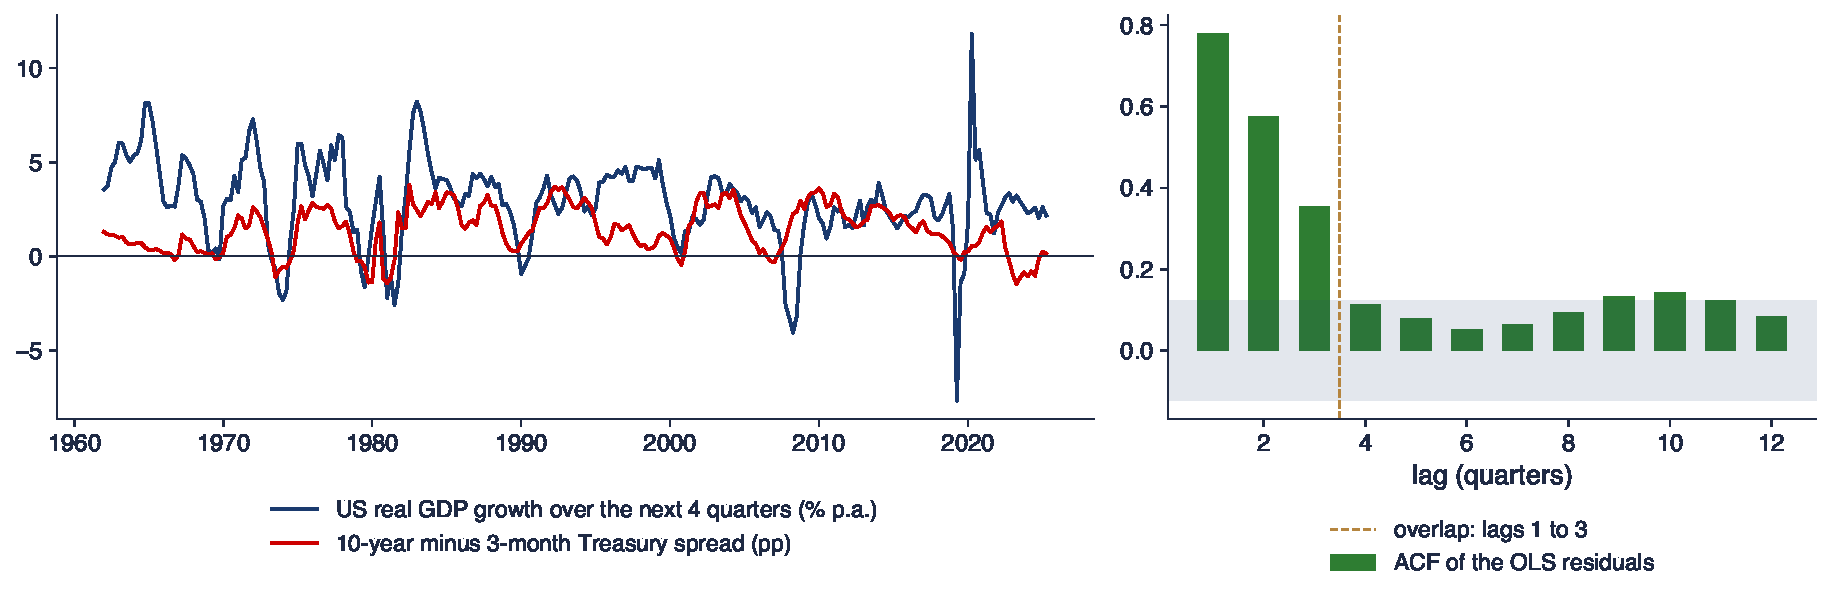
\includegraphics[width=0.97\textwidth,height=0.55\textheight,keepaspectratio]{ats_ch0_term_spread.pdf}
\end{center}
\vspace{-0.25cm}
\begin{itemize}
    \item Left: the two series; right: ACF of the OLS residuals, $\hat\rho_1 = 0.78$, $\hat\rho_3 = 0.35$, $\hat\rho_4 = 0.11$
\end{itemize}
\quantlet{ATS\_ch0\_term\_spread}{\qlurl{ATS_ch0_term_spread}}
\end{frame}

\begin{frame}{One slope, six standard errors}
\itemsize{\footnotesize}
\begin{center}
\footnotesize
\begin{tabular}{lrrr}
\toprule
Standard error & $\widehat{se}(\hat\beta_1)$ & $t$ & Critical value \\
\midrule
Classical OLS & 0.11 & 4.72 & $1.96$ \\
White (heteroskedasticity only) & 0.10 & -- & $1.96$ \\
Hansen--Hodrick, 3 lags & 0.20 & -- & $1.96$ \\
Newey--West, 3 lags & 0.17 & 3.10 & $1.96$ \\
NW, Andrews ($S = 14$) & 0.23 & 2.25 & $1.96$ \\
NW, $S = 1.3\sqrt{T} = 21$, fixed-$b$ & 0.25 & 2.04 & 2.18 \\
\bottomrule
\end{tabular}
\end{center}
\begin{itemize}
    \item $\hat\beta_1 = 0.52$ pp of annual growth per pp of spread, $R^2 = 0.08$
\end{itemize}
\end{frame}

\begin{frame}{Interpreting the term-spread regression}
\itemsize{\footnotesize}
\begin{itemize}
    \item The residuals are more persistent than the MA(3) implied by overlap ($\hat\rho_4 = 0.11$): 3 lags are not enough
    \begin{itemize}
        \item The standard error doubles from classical OLS to fixed-$b$: $t$ from $4.72$ to $2.04$, just below the critical value $2.18$
    \end{itemize}
    \item Subsamples (NW, 3 lags): 1962--1988 $\hat\beta_1 = 1.12$ ($t = 4.6$); 1989--2025 $\hat\beta_1 = 0.15$ ($t = 0.9$)
    \begin{itemize}
        \item The predictive power of the spread weakened after the original sample: a break question (\atschlink{https://danpele.github.io/Advanced-Time-Series/EN/Courses/chapter2_structural_breaks_nonlinear_models.pdf}{Chapter 2}) and an out-of-sample question (\atschlink{https://danpele.github.io/Advanced-Time-Series/EN/Courses/chapter1_forecast_evaluation.pdf}{Chapter 1})
    \end{itemize}
    \item Robust inference first, then stability: a full-sample $t$ of $4.72$ hides both problems
\end{itemize}
\end{frame}


%=============================================================================
\section{Multiple testing in forecasting research}
%=============================================================================

\begin{frame}{Data snooping}
\itemsize{\footnotesize}
\begin{itemize}
    \item \textbf{Data snooping}: reusing one data set to select a model, a rule or a specification, then testing it on the same data as if it were chosen in advance
    \begin{itemize}
        \item \refLM: sorting portfolios on characteristics already known to be related to returns biases asset-pricing tests
        \item \refHLZ: more than 300 published return factors; a new factor needs $t > 3$, not $t > 2$
    \end{itemize}
    \item Error rates for $K$ tests
    \begin{itemize}
        \item FWER (family-wise error rate): probability of at least one false rejection among the $K$ tests at level $\alpha$
        \item Bonferroni tests each hypothesis at $\alpha/K$; Holm (step-down; \refHolm) compares the ordered p-values $p_{(i)}$ with $\alpha/(K - i + 1)$; both control the FWER
        \item FDR (false discovery rate): expected share of false rejections among rejections, controlled by \refBH
    \end{itemize}
    \item In forecasting: many models, many horizons, many samples
    \begin{itemize}
        \item the honest $p$-value is the one of the \emph{search}, not of the winner
    \end{itemize}
\end{itemize}
\end{frame}

\begin{frame}{The best of $K$ tests}
\itemsize{\footnotesize}
\begin{center}
    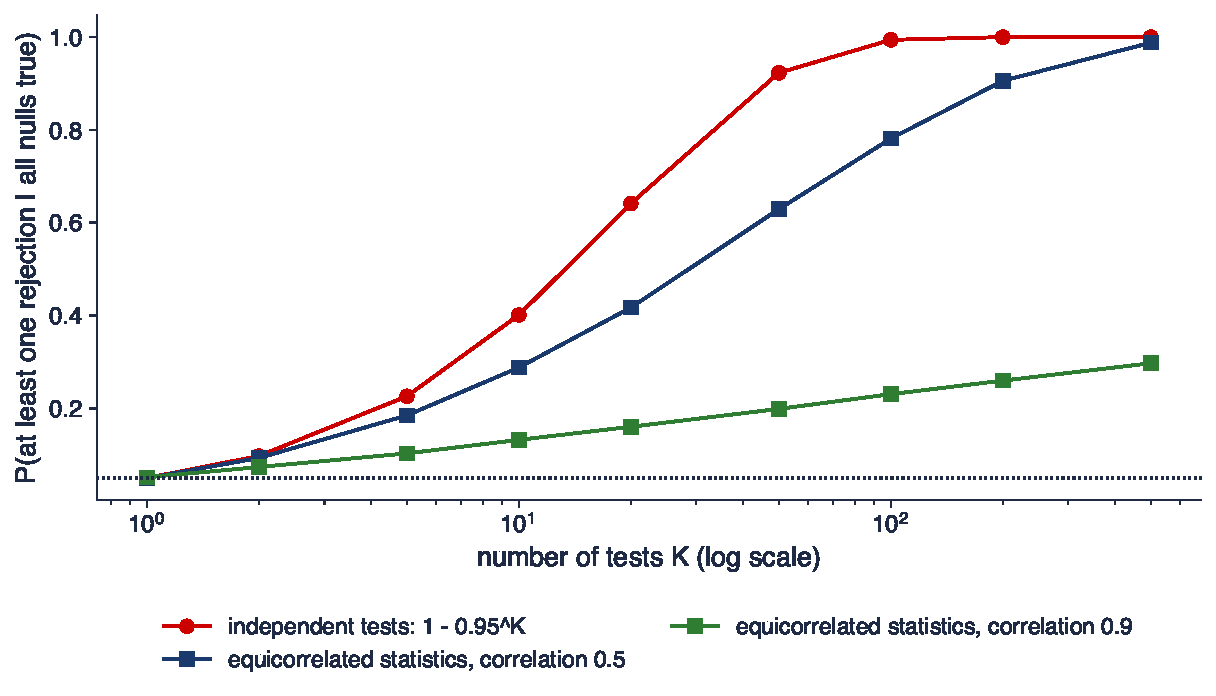
\includegraphics[width=0.97\textwidth,height=0.55\textheight,keepaspectratio]{ats_ch0_snooping.pdf}
\end{center}
\vspace{-0.25cm}
\begin{itemize}
    \item Probability that the largest $|t|$ of $K$ tests exceeds 1.96 when all nulls are true: independent and equicorrelated statistics (20\,000 simulations)
\end{itemize}
\quantlet{ATS\_ch0\_data\_snooping}{\qlurl{ATS_ch0_data_snooping}}
\end{frame}

\begin{frame}{Interpreting the family-wise error}
\itemsize{\small}
\begin{itemize}
    \item Independent tests: FWER $64\%$ with $K = 20$ and $99.4\%$ with $K = 100$
    \begin{itemize}
        \item Bonferroni would test each at $0.05/20 = 0.0025$
    \end{itemize}
    \item Correlated statistics (similar rules, overlapping samples): FWER $42\%$ ($K = 20$) and $78\%$ ($K = 100$) at correlation 0.5; $23\%$ at 0.9
    \begin{itemize}
        \item Bonferroni ignores the correlation and is conservative: the bootstrap of the maximum (next slide) uses it
    \end{itemize}
    \item What do you think? With 50 moving-average rules, how many ``significant'' rules do you expect by chance at 5\%?
    \begin{itemize}
        \item Answer: $50 \times 0.05 = 2.5$ if the rules were independent; correlated rules give fewer distinct rejections, but the best $t$ is still inflated
    \end{itemize}
\end{itemize}
\end{frame}

\begin{frame}{Case study: the Reality Check of White (2000) (1/2)}
\itemsize{\small}
\begin{itemize}
    \item $K$ models against a benchmark, evaluated on $n$ periods \refWhite
    \begin{itemize}
        \item $f_{k,t}$: the performance difference of model $k$ at $t$ (e.g.\ return of rule $k$ minus buy-and-hold); $\bar f_k$: its mean over the $n$ periods
    \end{itemize}
    \item Hypothesis and statistic
    \begin{itemize}
        \item $H_0: \max_k E f_{k,t} \le 0$ (no model beats the benchmark); $\quad \bar V = \max_k \sqrt{n}\,\bar f_k$
        \item $\bar V$: the scaled average outperformance of the best model; a large $\bar V$ is evidence against $H_0$
    \end{itemize}
\end{itemize}
\end{frame}

\begin{frame}{Case study: the Reality Check of White (2000) (2/2)}
\itemsize{\small}
\begin{itemize}
    \item Null distribution by the stationary bootstrap of the whole vector $f_t$ (keeps the correlation across rules and over time):
    \begin{itemize}
        \item $\bar V^*_b = \max_k \sqrt{n}\,(\bar f^*_{k,b} - \bar f_k)$, $\quad p = B^{-1}\sum_b \mathbf{1}\{\bar V^*_b > \bar V\}$
        \item $b = 1, \dots, B$: the resamples; $\bar f^*_{k,b}$: the mean of rule $k$ in resample $b$; $\mathbf{1}\{\cdot\}$: 1 if the condition holds, 0 otherwise
        \item $p$: the share of resamples with a larger maximum than the observed one, i.e.\ a $p$-value for the whole search
    \end{itemize}
    \item \refSTW{} apply it to 7846 technical rules on the Dow Jones; \refHansen{} (SPA) and \refRW{} (StepM) refine it: \atschlink{https://danpele.github.io/Advanced-Time-Series/EN/Courses/chapter1_forecast_evaluation.pdf}{Chapter 1}
    \item Our application: 50 rules ``long if the close is above its $n$-day moving average'', $n = 5, 10, \dots, 250$, on the BET
    \begin{itemize}
        \item against buy-and-hold, no costs; mean block of 10 days
    \end{itemize}
\end{itemize}
\end{frame}

\begin{frame}{The Reality Check on the BET}
\itemsize{\footnotesize}
\begin{center}
    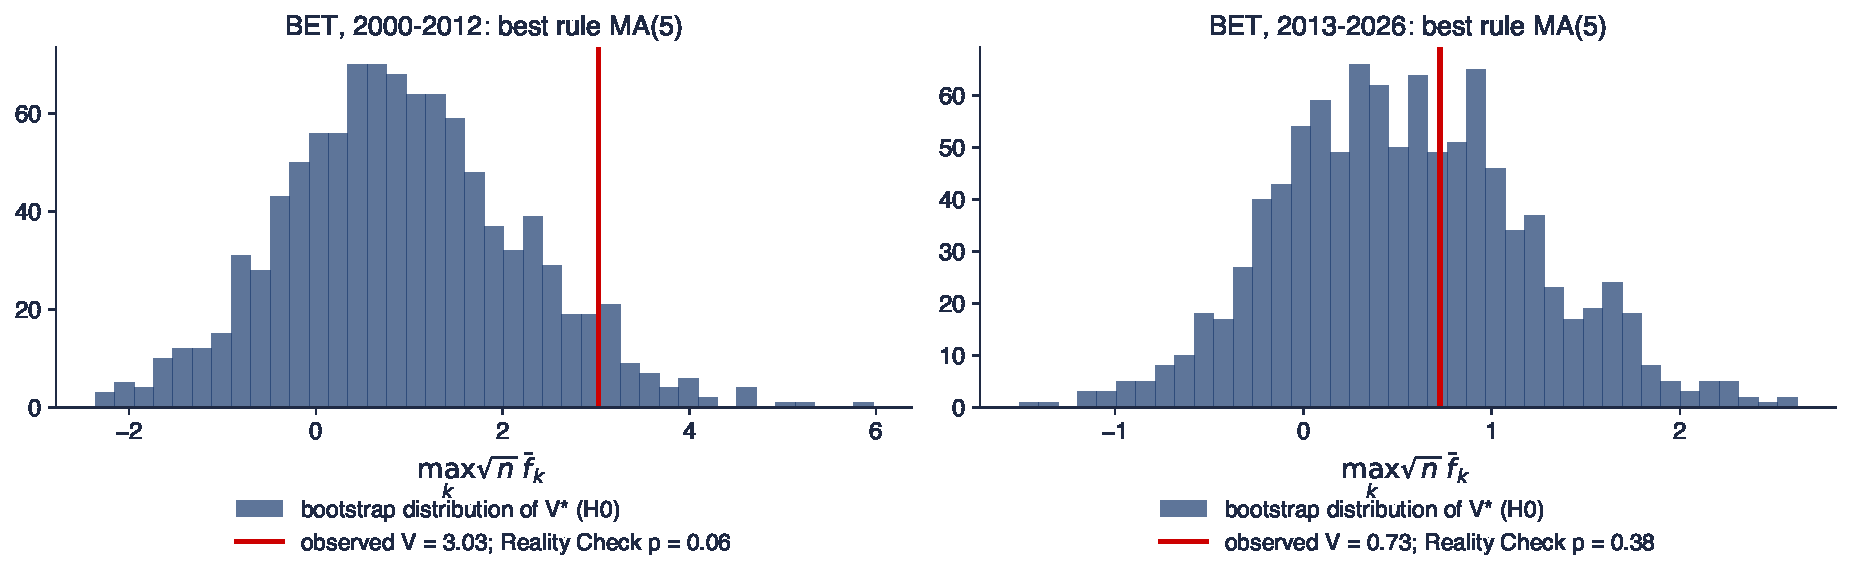
\includegraphics[width=0.97\textwidth,height=0.55\textheight,keepaspectratio]{ats_ch0_reality_check.pdf}
\end{center}
\vspace{-0.25cm}
\begin{itemize}
    \item Bootstrap distribution of $\bar V^*$ under $H_0$ (999 stationary-bootstrap resamples) and the observed $\bar V$; two subsamples
\end{itemize}
\quantlet{ATS\_ch0\_data\_snooping}{\qlurl{ATS_ch0_data_snooping}}
\end{frame}

\begin{frame}{Interpreting the Reality Check}
\itemsize{\footnotesize}
\begin{itemize}
    \item 2001--2012 ($n = 2\,993$ days): the best rule MA(5) beats buy-and-hold by $0.055\%$ a day, $t = 2.51$, naive one-sided $p = 0.006$
    \begin{itemize}
        \item Reality Check $p = 0.06$: not significant at 5\% once the search over 50 rules is accounted for
    \end{itemize}
    \item 2014--2026: the same rule, $t = 0.97$, Reality Check $p = 0.38$: whatever existed did not survive
    \item The short-MA winner fits the positive $\hat\rho_1$ of BET returns (stale prices)
    \begin{itemize}
        \item transaction costs would eat the gain
    \end{itemize}
    \item Pre-register the rule universe and the sample split before looking at the results (Stage 1 of the project)
\end{itemize}
\end{frame}

\begin{frame}{Recap: multiple testing}
\itemsize{\small}
\begin{itemize}
    \item The $p$-value of the best of $K$ is not the $p$-value of a pre-specified test
    \item FWER (Bonferroni, Holm) or FDR (Benjamini--Hochberg); for correlated forecasts: bootstrap the maximum (Reality Check)
    \item Forecast comparison tests (Diebold--Mariano, SPA, Model Confidence Set) are the subject of \atschlink{https://danpele.github.io/Advanced-Time-Series/EN/Courses/chapter1_forecast_evaluation.pdf}{Chapter 1}
\end{itemize}
\end{frame}


%=============================================================================
\section{Reproducible research practice}
%=============================================================================

\begin{frame}{Seeds and Monte Carlo experiments}
\itemsize{\small}
\begin{itemize}
    \item One seed per project, set once: \texttt{rng = np.random.default\_rng(2026)}; pass \texttt{rng} to every function
    \begin{itemize}
        \item Parallel runs: \texttt{np.random.SeedSequence(2026).spawn(k)} gives independent streams; never reuse a global state
    \end{itemize}
    \item Report what makes a simulation checkable
    \begin{itemize}
        \item DGP, $T$, number of replications $R$, burn-in, seed, Monte Carlo standard error $\sqrt{p(1-p)/R}$
        \item Results must not depend on the seed beyond the Monte Carlo error: rerun with a second seed
    \end{itemize}
    \item Every chart and every number of this chapter is produced by one script with seed 2026 (Quantlets/Ch\_00)
\end{itemize}
\end{frame}

\begin{frame}{Versioned data}
\itemsize{\small}
\begin{itemize}
    \item Macro data are revised: the GDP you download today is not the GDP a forecaster saw in real time
    \begin{itemize}
        \item Real-time vintages: \refCS{} (Philadelphia Fed), ALFRED for FRED series; Eurostat revises national accounts every quarter
    \end{itemize}
    \item Save a dated snapshot of every series used, with the query that produced it
    \begin{itemize}
        \item Record the download date, the dataset code (e.g.\ \texttt{namq\_10\_gdp}) and a checksum (\texttt{sha256}) of the file
        \item The course market data are saved once and end on 18 September 2026: every student gets the same numbers
    \end{itemize}
    \item A forecast evaluated on revised data answers a different question than the one asked in real time
\end{itemize}
\end{frame}

\begin{frame}{Replication packages}
\itemsize{\small}
\begin{itemize}
    \item What economics journals now require \refVilhuber, \refCM
    \begin{itemize}
        \item a README with a data availability statement, the order of the scripts and the expected run time
        \item code that regenerates every table and figure from raw data, without manual steps
        \item the computational environment: \texttt{requirements.txt} with versions, or a Colab notebook
    \end{itemize}
    \item For the ATS project (Stage 2)
    \begin{itemize}
        \item a GitHub repository: \texttt{data/}, \texttt{code/}, \texttt{output/}, README, AI\_USE.md, AI\_ERRORS.md
        \item one command or one notebook reproduces every number in the report
    \end{itemize}
    \item Test: a colleague clones the repository on a clean machine and gets the same numbers
\end{itemize}
\end{frame}

\begin{frame}{Pre-registration and the analysis plan}
\itemsize{\small}
\begin{itemize}
    \item Stage 1 of the project fixes, before any estimation:
    \begin{itemize}
        \item the hypothesis, the sample and its split (estimation, evaluation), the benchmark
        \item the inference method (HAC rule, bootstrap, critical values) and the multiple-testing correction
        \item the list of specifications that will be reported, all of them
    \end{itemize}
    \item Why: the garden of forking paths turns many small choices into an implicit search
    \begin{itemize}
        \item Every deviation from the plan is allowed but reported, with its reason
    \end{itemize}
    \item An AI assistant makes the search cheaper: AI\_USE.md records the prompts that shaped a decision
\end{itemize}
\end{frame}

\begin{frame}{Recap: reproducible research}
\itemsize{\small}
\begin{itemize}
    \item Seed once, pass the generator, report $R$ and the Monte Carlo error
    \item Dated, checksummed data snapshots; real-time vintages when the question is about real-time forecasting
    \item A replication package that runs from raw data to every number; a plan fixed before the results
\end{itemize}
\end{frame}


%=============================================================================
\section{AI for scientific discovery}
%=============================================================================

\begin{frame}{An open question: valid inference for a near-integrated mean}
\itemsize{\small}
\begin{itemize}
    \item Has Romanian inflation averaged the BNR target since 2013? Formally, $H_0: \mu = 2.5$ for the HICP annual rate, 164 months to August 2026
    \begin{itemize}
        \item $\hat\rho_1 = 0.99$: the series is close to a unit root, and overlapping by construction
    \end{itemize}
    \item Open: no kernel, EWC or bootstrap rule controls size at this persistence (Monte Carlo above)
    \begin{itemize}
        \item \refMuller{} and \refLLS{} map the frontier; which test should a central-bank watcher use with 10--15 years of data?
    \end{itemize}
    \item A question with policy content (credibility of the target) and a methodological core (HAR inference at $\phi \approx 1$)
\end{itemize}
\end{frame}

\begin{frame}{The AI-assisted discovery loop}
\itemsize{\footnotesize}
\begin{itemize}
    \item \textbf{Literature}: \aiprompt{"List peer-reviewed tests for the mean of a highly persistent series since 2010, with DOI and the Monte Carlo design."}
    \begin{itemize}
        \item Check: resolve every DOI on Crossref; read the size tables yourself (Semantic Scholar, Elicit for search)
    \end{itemize}
    \item \textbf{Hypothesis and code}: \aiprompt{"Write Python for NW fixed-b and EWC tests of a mean, and a Monte Carlo of their size at phi = 0.98, T = 164."}
    \begin{itemize}
        \item Check: reproduce a published size number first (e.g.\ the LLSW tables), then change one thing at a time
    \end{itemize}
    \item \textbf{Robustness and critique}: \aiprompt{"Act as a hostile referee: why could this test of the inflation mean be misleading?"}
    \begin{itemize}
        \item Expect: breaks in the mean (2013, 2022), the CPI--HICP gap, overlap, the choice of start date
    \end{itemize}
    \item \textbf{The human checks}: formulas, timing of information (no look-ahead), every number against the code; the tools are generic (Claude, ChatGPT, Gemini, Copilot)
\end{itemize}
\end{frame}

\begin{frame}{Mini-case: one hypothesis, six answers}
\itemsize{\footnotesize}
\begin{center}
    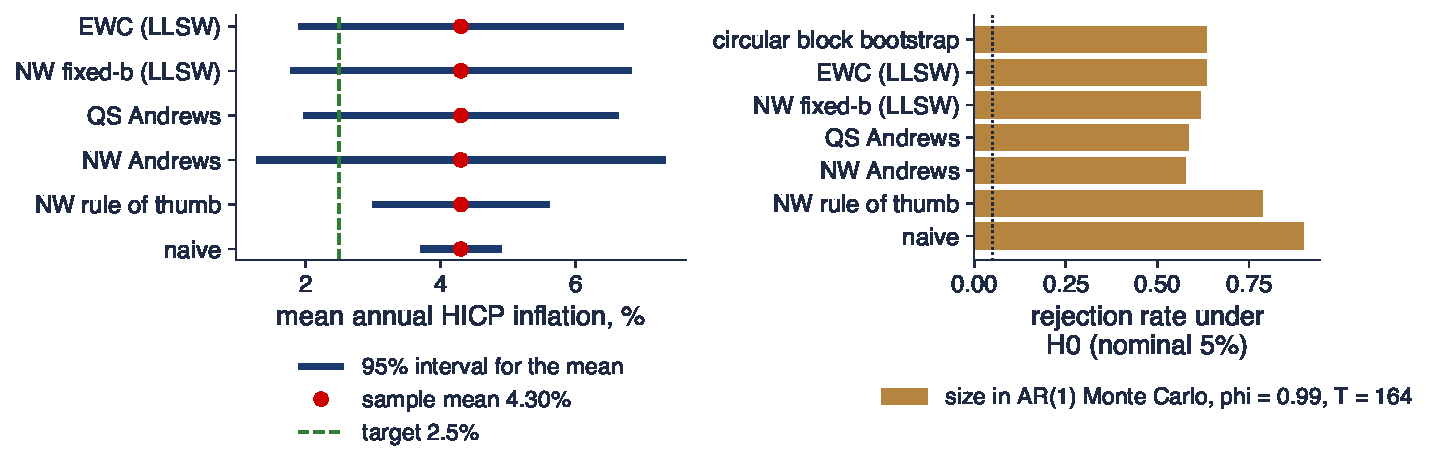
\includegraphics[width=0.97\textwidth,height=0.52\textheight,keepaspectratio]{ats_ch0_ai_minicase.pdf}
\end{center}
\vspace{-0.25cm}
\begin{itemize}
    \item Left: 95\% intervals for the mean HICP inflation since 2013 (mean $4.30\%$); right: size of each test in a Monte Carlo with the fitted AR(1), $\phi = 0.99$, $T = 164$
\end{itemize}
\quantlet{ATS\_ch0\_ai\_discovery}{\qlurl{ATS_ch0_ai_discovery}}
\end{frame}

\begin{frame}{Interpreting the mini-case}
\itemsize{\footnotesize}
\begin{itemize}
    \item A typical assistant proposal: ``NW with $\lfloor 4(T/100)^{2/9}\rfloor$ lags'' gives $t = 2.69$ and rejects $\mu = 2.5$
    \begin{itemize}
        \item Its actual size at this persistence: $79\%$ instead of 5\%; the naive test: $90\%$
    \end{itemize}
    \item NW-Andrews ($t = 1.17$), fixed-$b$ ($t = 1.59$, critical value $2.23$) and EWC ($t = 1.63$, $\nu = 12$) do not reject
    \begin{itemize}
        \item But their sizes are still $58\%$--$63\%$: a non-rejection is not evidence for the target either
    \end{itemize}
    \item Honest conclusion: with 14 years of a near-integrated series the data cannot settle the question; that is the open part
\end{itemize}
\end{frame}

\begin{frame}{Project idea}
\itemsize{\footnotesize}
\begin{itemize}
    \item \textbf{Question}: which HAR test is reliable for the mean of Romanian and euro-area inflation, 2005--2026?
    \begin{itemize}
        \item Replicate first: one size table of \refLLSW{} (their AR(1) design); explain every gap
    \end{itemize}
    \item \textbf{Extension}
    \begin{itemize}
        \item add the tests of \refMuller; calibrate the Monte Carlo to HICP data of all EU countries (Eurostat)
        \item report size and power on one frontier per country; test the target hypothesis with the test that controls size
    \end{itemize}
    \item \textbf{Deliverables}: a dated pre-analysis plan; a replication package; AI\_USE.md with the prompts that shaped decisions; AI\_ERRORS.md with each invented reference or wrong number caught
\end{itemize}
\end{frame}


%=============================================================================
\section{Conclusions}
%=============================================================================

\begin{frame}{Key takeaways}
\itemsize{\small}
\begin{itemize}
    \item The precision of a mean or a slope is governed by the long-run variance $\Omega = 2\pi f(0)$, not by $\gamma_0$
    \item Ergodicity gives consistency; MDS or mixing structure gives the CLT; the HAC estimator gives the standard error
    \item Kernel, bandwidth and critical values are one decision: NW with $1.3\sqrt{T}$ and fixed-$b$, or EWC, by default
    \item Block bootstraps resample dependence; the wild bootstrap does not
    \item Near unit roots defeat all of them: measure the size of your test by Monte Carlo at your persistence
    \item Searches need search-adjusted $p$-values; projects need replication packages and a plan fixed in advance
\end{itemize}
\end{frame}

\begin{frame}{Self-assessment}
\itemsize{\small}
\begin{itemize}
    \item What is the long-run variance of an MA(1) with $\theta = -0.5$ and $\sigma^2 = 1$?
    \item Why can the truncated kernel give a negative variance while the Bartlett kernel cannot?
    \item Which standard error would you use for the mean of daily S\&P 500 returns?
    \item Which standard error would you use for the mean of their squares?
    \item Why is the wild bootstrap invalid for a regression with overlapping four-quarter growth?
    \item You tried 40 specifications and report the best one: which $p$-value should you report?
\end{itemize}
\end{frame}

\begin{frame}{Next chapter and further reading}
\itemsize{\small}
\begin{itemize}
    \item \textbf{Next}: \atschlink{https://danpele.github.io/Advanced-Time-Series/EN/Courses/chapter1_forecast_evaluation.pdf}{Chapter 1}, forecast evaluation, scoring rules and combination
    \begin{itemize}
        \item Diebold--Mariano is a HAC $t$-test on loss differentials; SPA and the Model Confidence Set use the stationary bootstrap of this chapter
    \end{itemize}
    \item \textbf{Further reading}
    \begin{itemize}
        \item Theory: \refHamilton{} (Ch.\ 7 and 10), \refBradley, \refLahiri
        \item Practice: \refLLSW, \refLLS, \refMuller
        \item Snooping: \refWhite, \refHansen, \refRW, \refHLZ
    \end{itemize}
    \item \textbf{Code}
    \begin{itemize}
        \item Quantlets: \href{https://github.com/danpele/Advanced-Time-Series/tree/main/Quantlets/Ch_00}{github.com/danpele/Advanced-Time-Series/tree/main/Quantlets/Ch\_00}
        \item Python: \texttt{statsmodels} (\texttt{cov\_type="HAC"}), \texttt{arch.bootstrap} (\texttt{StationaryBootstrap}, \texttt{optimal\_block\_length}, \texttt{SPA})
    \end{itemize}
\end{itemize}
\end{frame}


%=============================================================================
\section{References}
%=============================================================================

\begin{frame}{References (1/4)}
\itemsize{\tiny}
\begin{itemize}
    \item Andrews, D.W.K. (1991). \href{https://doi.org/10.2307/2938229}{Heteroskedasticity and autocorrelation consistent covariance matrix estimation}. \emph{Econometrica}, 59(3), 817--858.
    \item Andrews, D.W.K., Monahan, J.C. (1992). \href{https://doi.org/10.2307/2951574}{An improved heteroskedasticity and autocorrelation consistent covariance matrix estimator}. \emph{Econometrica}, 60(4), 953--966.
    \item Angelopoulos, A.N., Bates, S. (2023). \href{https://doi.org/10.1561/2200000101}{Conformal prediction: a gentle introduction}. \emph{Foundations and Trends in Machine Learning}, 16(4), 494--591.
    \item Baltagi, B.H. (2021). \href{https://doi.org/10.1007/978-3-030-53953-5}{\emph{Econometric Analysis of Panel Data}} (6th ed.). Springer.
    \item Benjamini, Y., Hochberg, Y. (1995). \href{https://doi.org/10.1111/j.2517-6161.1995.tb02031.x}{Controlling the false discovery rate: a practical and powerful approach to multiple testing}. \emph{Journal of the Royal Statistical Society B}, 57(1), 289--300.
    \item Billingsley, P. (1961). \href{https://doi.org/10.1090/S0002-9939-1961-0126871-X}{The Lindeberg--Lévy theorem for martingales}. \emph{Proceedings of the American Mathematical Society}, 12(5), 788--792.
    \item Birkhoff, G.D. (1931). \href{https://doi.org/10.1073/pnas.17.2.656}{Proof of the ergodic theorem}. \emph{Proceedings of the National Academy of Sciences}, 17(12), 656--660.
    \item Bradley, R.C. (2005). \href{https://doi.org/10.1214/154957805100000104}{Basic properties of strong mixing conditions. A survey and some open questions}. \emph{Probability Surveys}, 2, 107--144.
    \item Brown, B.M. (1971). \href{https://doi.org/10.1214/aoms/1177693494}{Martingale central limit theorems}. \emph{The Annals of Mathematical Statistics}, 42(1), 59--66.
    \item Bühlmann, P. (1997). \href{https://doi.org/10.2307/3318584}{Sieve bootstrap for time series}. \emph{Bernoulli}, 3(2), 123--148.
    \item Carrasco, M., Chen, X. (2002). \href{https://doi.org/10.1017/S0266466602181023}{Mixing and moment properties of various GARCH and stochastic volatility models}. \emph{Econometric Theory}, 18(1), 17--39.
    \item Christensen, G., Miguel, E. (2018). \href{https://doi.org/10.1257/jel.20171350}{Transparency, reproducibility, and the credibility of economics research}. \emph{Journal of Economic Literature}, 56(3), 920--980.
    \item Croushore, D., Stark, T. (2001). \href{https://doi.org/10.1016/S0304-4076(01)00072-0}{A real-time data set for macroeconomists}. \emph{Journal of Econometrics}, 105(1), 111--130.
    \item Durbin, J., Koopman, S.J. (2012). \href{https://doi.org/10.1093/acprof:oso/9780199641178.001.0001}{\emph{Time Series Analysis by State Space Methods}} (2nd ed.). Oxford University Press.
    \item Efron, B. (1979). \href{https://doi.org/10.1214/aos/1176344552}{Bootstrap methods: another look at the jackknife}. \emph{The Annals of Statistics}, 7(1), 1--26.
\end{itemize}
\end{frame}

\begin{frame}{References (2/4)}
\itemsize{\tiny}
\begin{itemize}
    \item Estrella, A., Hardouvelis, G.A. (1991). \href{https://doi.org/10.1111/j.1540-6261.1991.tb02674.x}{The term structure as a predictor of real economic activity}. \emph{The Journal of Finance}, 46(2), 555--576.
    \item Gonçalves, S., Kilian, L. (2004). \href{https://doi.org/10.1016/j.jeconom.2003.10.030}{Bootstrapping autoregressions with conditional heteroskedasticity of unknown form}. \emph{Journal of Econometrics}, 123(1), 89--120.
    \item Granger, C.W.J., Newbold, P. (1974). \href{https://doi.org/10.1016/0304-4076(74)90034-7}{Spurious regressions in econometrics}. \emph{Journal of Econometrics}, 2(2), 111--120.
    \item Hamilton, J.D. (1994). \href{https://doi.org/10.2307/j.ctv14jx6sm}{\emph{Time Series Analysis}}. Princeton University Press.
    \item Hansen, L.P., Hodrick, R.J. (1980). \href{https://doi.org/10.1086/260910}{Forward exchange rates as optimal predictors of future spot rates: an econometric analysis}. \emph{Journal of Political Economy}, 88(5), 829--853.
    \item Hansen, P.R. (2005). \href{https://doi.org/10.1198/073500105000000063}{A test for superior predictive ability}. \emph{Journal of Business \& Economic Statistics}, 23(4), 365--380.
    \item Harvey, C.R., Liu, Y., Zhu, H. (2016). \href{https://doi.org/10.1093/rfs/hhv059}{\ldots and the cross-section of expected returns}. \emph{The Review of Financial Studies}, 29(1), 5--68.
    \item Holm, S. (1979). \href{https://www.jstor.org/stable/4615733}{A simple sequentially rejective multiple test procedure}. \emph{Scandinavian Journal of Statistics}, 6(2), 65--70.
    \item Huang, C., Petukhina, A. (2022). \href{https://doi.org/10.1007/978-3-031-13584-2}{\emph{Applied Time Series Analysis and Forecasting with Python}}. Springer.
    \item Hyndman, R.J., Athanasopoulos, G. (2021). \href{https://otexts.com/fpp3/}{\emph{Forecasting: Principles and Practice}} (3rd ed.). OTexts.
    \item Ibragimov, I.A. (1962). \href{https://doi.org/10.1137/1107036}{Some limit theorems for stationary processes}. \emph{Theory of Probability and Its Applications}, 7(4), 349--382.
    \item Kiefer, N.M., Vogelsang, T.J. (2002). \href{https://doi.org/10.1111/1468-0262.00366}{Heteroskedasticity-autocorrelation robust standard errors using the Bartlett kernel without truncation}. \emph{Econometrica}, 70(5), 2093--2095.
    \item Kiefer, N.M., Vogelsang, T.J. (2005). \href{https://doi.org/10.1017/S0266466605050565}{A new asymptotic theory for heteroskedasticity-autocorrelation robust tests}. \emph{Econometric Theory}, 21(6), 1130--1164.
    \item Kiefer, N.M., Vogelsang, T.J., Bunzel, H. (2000). \href{https://doi.org/10.1111/1468-0262.00128}{Simple robust testing of regression hypotheses}. \emph{Econometrica}, 68(3), 695--714.
    \item Kilian, L., Lütkepohl, H. (2017). \href{https://doi.org/10.1017/9781108164818}{\emph{Structural Vector Autoregressive Analysis}}. Cambridge University Press.
\end{itemize}
\end{frame}

\begin{frame}{References (3/4)}
\itemsize{\tiny}
\begin{itemize}
    \item Künsch, H.R. (1989). \href{https://doi.org/10.1214/aos/1176347265}{The jackknife and the bootstrap for general stationary observations}. \emph{The Annals of Statistics}, 17(3), 1217--1241.
    \item Lahiri, S.N. (2003). \href{https://doi.org/10.1007/978-1-4757-3803-2}{\emph{Resampling Methods for Dependent Data}}. Springer.
    \item Lazarus, E., Lewis, D.J., Stock, J.H. (2021). \href{https://doi.org/10.3982/ECTA15404}{The size-power tradeoff in HAR inference}. \emph{Econometrica}, 89(5), 2497--2516.
    \item Lazarus, E., Lewis, D.J., Stock, J.H., Watson, M.W. (2018). \href{https://doi.org/10.1080/07350015.2018.1506926}{HAR inference: recommendations for practice}. \emph{Journal of Business \& Economic Statistics}, 36(4), 541--559.
    \item Liu, R.Y. (1988). \href{https://doi.org/10.1214/aos/1176351062}{Bootstrap procedures under some non-i.i.d.\ models}. \emph{The Annals of Statistics}, 16(4), 1696--1708.
    \item Lo, A.W., MacKinlay, A.C. (1990). \href{https://doi.org/10.1093/rfs/3.3.431}{Data-snooping biases in tests of financial asset pricing models}. \emph{The Review of Financial Studies}, 3(3), 431--467.
    \item Lütkepohl, H. (2005). \href{https://doi.org/10.1007/978-3-540-27752-1}{\emph{New Introduction to Multiple Time Series Analysis}}. Springer.
    \item Mammen, E. (1993). \href{https://doi.org/10.1214/aos/1176349025}{Bootstrap and wild bootstrap for high dimensional linear models}. \emph{The Annals of Statistics}, 21(1), 255--285.
    \item Mokkadem, A. (1988). \href{https://doi.org/10.1016/0304-4149(88)90045-2}{Mixing properties of ARMA processes}. \emph{Stochastic Processes and their Applications}, 29(2), 309--315.
    \item Müller, U.K. (2014). \href{https://doi.org/10.1080/07350015.2014.931238}{HAC corrections for strongly autocorrelated time series}. \emph{Journal of Business \& Economic Statistics}, 32(3), 311--322.
    \item Newey, W.K., West, K.D. (1987). \href{https://doi.org/10.2307/1913610}{A simple, positive semi-definite, heteroskedasticity and autocorrelation consistent covariance matrix}. \emph{Econometrica}, 55(3), 703--708.
    \item Newey, W.K., West, K.D. (1994). \href{https://doi.org/10.2307/2297912}{Automatic lag selection in covariance matrix estimation}. \emph{The Review of Economic Studies}, 61(4), 631--653.
    \item Patton, A., Politis, D.N., White, H. (2009). \href{https://doi.org/10.1080/07474930802459016}{Correction to ``Automatic block-length selection for the dependent bootstrap''}. \emph{Econometric Reviews}, 28(4), 372--375.
    \item Petropoulos, F., Apiletti, D., Assimakopoulos, V., Babai, M.Z., et al.\ (2022). \href{https://doi.org/10.1016/j.ijforecast.2021.11.001}{Forecasting: theory and practice}. \emph{International Journal of Forecasting}, 38(3), 705--871.
    \item Phillips, P.C.B. (1986). \href{https://doi.org/10.1016/0304-4076(86)90001-1}{Understanding spurious regressions in econometrics}. \emph{Journal of Econometrics}, 33(3), 311--340.
\end{itemize}
\end{frame}

\begin{frame}{References (4/4)}
\itemsize{\tiny}
\begin{itemize}
    \item Phillips, P.C.B., Solo, V. (1992). \href{https://doi.org/10.1214/aos/1176348666}{Asymptotics for linear processes}. \emph{The Annals of Statistics}, 20(2), 971--1001.
    \item Politis, D.N., Romano, J.P. (1992). \href{https://openlibrary.org/books/OL1551704M}{A circular block-resampling procedure for stationary data}. In R. LePage, L. Billard (Eds.), \emph{Exploring the Limits of Bootstrap} (pp. 263--270). Wiley.
    \item Politis, D.N., Romano, J.P. (1994). \href{https://doi.org/10.1080/01621459.1994.10476870}{The stationary bootstrap}. \emph{Journal of the American Statistical Association}, 89(428), 1303--1313.
    \item Politis, D.N., White, H. (2004). \href{https://doi.org/10.1081/ETC-120028836}{Automatic block-length selection for the dependent bootstrap}. \emph{Econometric Reviews}, 23(1), 53--70.
    \item Romano, J.P., Wolf, M. (2005). \href{https://doi.org/10.1111/j.1468-0262.2005.00615.x}{Stepwise multiple testing as formalized data snooping}. \emph{Econometrica}, 73(4), 1237--1282.
    \item Rosenblatt, M. (1956). \href{https://doi.org/10.1073/pnas.42.1.43}{A central limit theorem and a strong mixing condition}. \emph{Proceedings of the National Academy of Sciences}, 42(1), 43--47.
    \item Shao, X. (2010). \href{https://doi.org/10.1198/jasa.2009.tm08744}{The dependent wild bootstrap}. \emph{Journal of the American Statistical Association}, 105(489), 218--235.
    \item Shumway, R.H., Stoffer, D.S. (2017). \href{https://doi.org/10.1007/978-3-319-52452-8}{\emph{Time Series Analysis and Its Applications}} (4th ed.). Springer.
    \item Singh, K. (1981). \href{https://doi.org/10.1214/aos/1176345636}{On the asymptotic accuracy of Efron's bootstrap}. \emph{The Annals of Statistics}, 9(6), 1187--1195.
    \item Sullivan, R., Timmermann, A., White, H. (1999). \href{https://doi.org/10.1111/0022-1082.00163}{Data-snooping, technical trading rule performance, and the bootstrap}. \emph{The Journal of Finance}, 54(5), 1647--1691.
    \item Sun, Y., Phillips, P.C.B., Jin, S. (2008). \href{https://doi.org/10.1111/j.0012-9682.2008.00822.x}{Optimal bandwidth selection in heteroskedasticity--autocorrelation robust testing}. \emph{Econometrica}, 76(1), 175--194.
    \item Vilhuber, L. (2020). \href{https://doi.org/10.1162/99608f92.4f6b9e67}{Reproducibility and replicability in economics}. \emph{Harvard Data Science Review}, 2(4).
    \item White, H. (1980). \href{https://doi.org/10.2307/1912934}{A heteroskedasticity-consistent covariance matrix estimator and a direct test for heteroskedasticity}. \emph{Econometrica}, 48(4), 817--838.
    \item White, H. (2000). \href{https://doi.org/10.1111/1468-0262.00152}{A reality check for data snooping}. \emph{Econometrica}, 68(5), 1097--1126.
    \item Wu, C.F.J. (1986). \href{https://doi.org/10.1214/aos/1176350142}{Jackknife, bootstrap and other resampling methods in regression analysis}. \emph{The Annals of Statistics}, 14(4), 1261--1295.
\end{itemize}
\end{frame}

\end{document}
